\documentclass[a4paper,oneside]{report}
%\documentclass[a4paper]{ctexart}

\usepackage{amssymb}
\usepackage{amsmath}
\usepackage{CJKutf8}
\usepackage{color}
\usepackage{enumerate}
\usepackage{fancyhdr}
\usepackage{geometry}
\usepackage{graphicx}
\usepackage{indentfirst}
\usepackage{latexsym}
\usepackage{mathrsfs}
\usepackage{subfigure}
\usepackage{textcomp}
\usepackage{url}
%\usepackage{unicode-math}

\usepackage{flafter}
\usepackage{booktabs, longtable}
\usepackage{pxfonts}
\usepackage{cite}

\DeclareMathAlphabet{\mathcal}{OMS}{cmsy}{m}{n}
\let\mathbb\relax % remove the definition by unicode-math
\DeclareMathAlphabet{\mathbb}{U}{msb}{m}{n}

\begin{document}
%\begin{CJK*}{UTF8}{gbsn}
\begin{CJK*}{UTF8}{gkai}
\CJKindent
%------------中文设置--------------------------
\makeatletter %将文献引用作为上标出现,增加括号,
\def\@cite#1#2{\textsuperscript{[{#1\if@tempswa , #2\fi}]}}
\makeatother
\newtheorem{theorem}{{定理}}
\newtheorem{remark}{{注}}
\newtheorem{proposition}[theorem]{{命题}}
\newtheorem{lemma}[theorem]{{引理}}
\newtheorem{corollary}[theorem]{{推论}}
\newtheorem{definition}[theorem]{{定义}}
\newtheorem{question}[theorem]{{问题}}

%\renewcommand{\refname}{\centerline{参考文献}}
\renewcommand{\bibname}{\centerline{参考文献}}
\renewcommand{\tablename}{表}
%\renewcommand{\captionlabeldelim}{\quad}
%===================Image settings========================%
\renewcommand{\figurename}{图}
%\renewcommand{\abstractname}{摘要}
%\renewcommand{\captionlabeldelim}{\quad} %Need caption2 macro package
%===============End image settings========================%
%-----------中文设置--------------------------

		
\title{科研新手快速入门指南}
\author{朱玉可 (\texttt{yukezhu0323@126.com})\\
  张庆海 (\texttt{qinghai@zju.edu.cn})\\
}
\date{浙江大学数学科学学院计算数学系}


\maketitle

%
\begin{center}
  \large
  序言
\end{center}

好的学习工具和思想方法可以让学习变的更加高效。
本书中总结的内容覆盖了张庆海老师研究团队的研究生必须掌握的基本工具和科
研方法。
第1章主要介绍一些科学计算中的常用工具,
从新系统的安装到其上一些软件(emacs,texlive,make,gdb 等等)的使用。
熟练的运用这些软件,往往可以达到事半功倍的效果;
第2章简单的介绍一些重要的思想及良好的习惯。
在以后的学习生涯中,养成这些习惯,贯彻这些思想,并融汇贯通,
将使你的科研大有裨益。


%%% Local Variables:
%%% mode: latex
%%% TeX-master: "../Guide"
%%% End:


\pagestyle{empty}

\tableofcontents
\clearpage

\pagestyle{fancy}
\fancyhead{}
\lhead{朱玉可}
\chead{}
\rhead{入门指南}


\chapter{工具篇}

\section{Ubuntu 操作系统及其上软件的安装}
\label{sec:ubuntu}
\subsection{安装 Ubuntu 操作系统}

如果你只需要处理一般的事务,打游戏,那么你不需要了解下面这些了。
但是其实世界上的大多数科学家和工程师几乎用的都是 Linux 系统作为他们的电脑工具。
就因为它简单,可靠,稳定,强大,有趣。
甚至很多时候 Linux 就是唯一的选择。
Ubuntu 作为当下非常流行的 Linux 发行版,
在桌面办公、服务器方面都有着不俗的表现。
在接触一个新的系统之前,学会安装是深入了解它的前提。

使用一个 Linux 操作系统的方式有很多,常见的有虚拟机和双系统两种方式。
这里我们主要介绍一下双系统 (Win10 + Ubuntu) 的安装。

\begin{itemize}
	\item [I.] 准备工作
		\begin{itemize}
			\item [I-a.] 磁盘分区:
			    首先查看本机的磁盘情况(win+x $\to$ Disk Management)。
				在足够大的硬盘上选择合适的大小进行压缩(右键$\to$Shink Volume),
				压缩卷的大小即为即将安装的Ubuntu系统的大小,推荐为60GB以上(建议120GB)。
				压缩后磁盘出现空白卷,如图 (\ref{fig:shrinkVol})
				\begin{figure}[htbp]
					\centering
					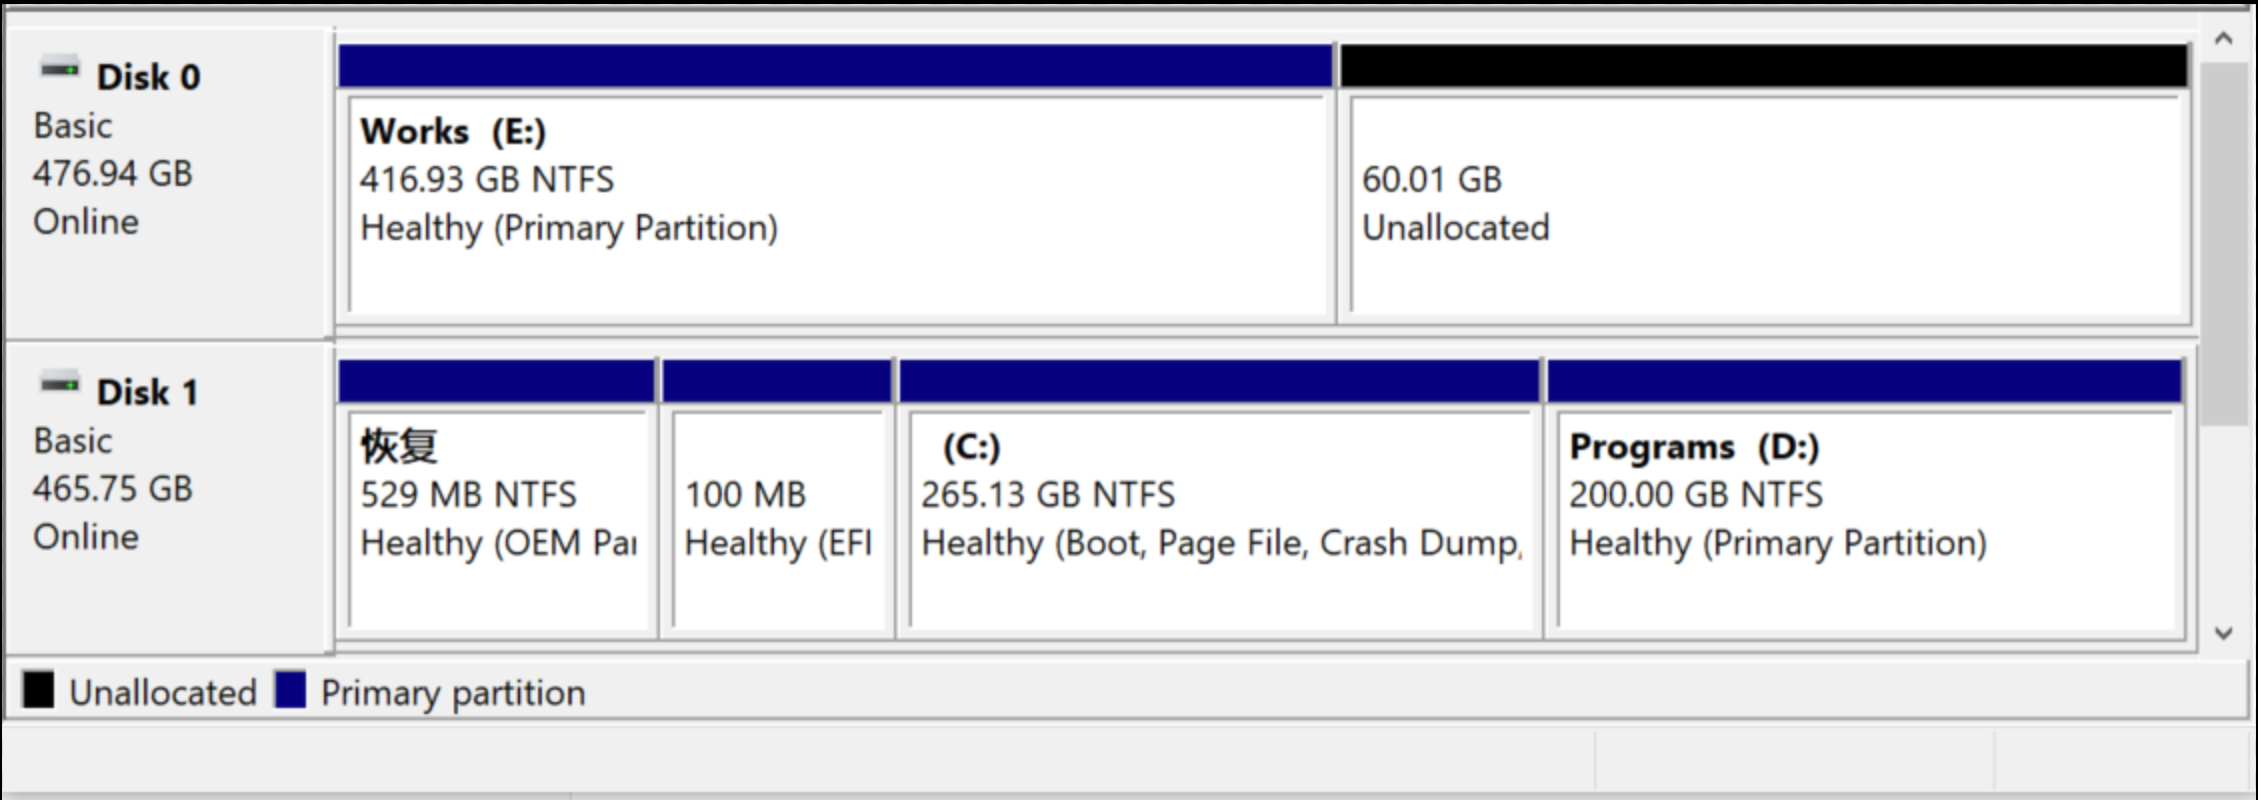
\includegraphics[width=0.7\textwidth]{png/shrinkVol}
					\caption{压缩后的磁盘出现空白卷(Unallocated)。}
					\label{fig:shrinkVol}
				\end{figure}
			\item [I-b.] 下载系统镜像:从 Ubuntu 官网下载最新安装镜像,
				下载地址为
				\begin{verbatim}
				https://ubuntu.com/download/desktop.
				\end{verbatim}
				\begin{figure}[htbp]
					\centering
					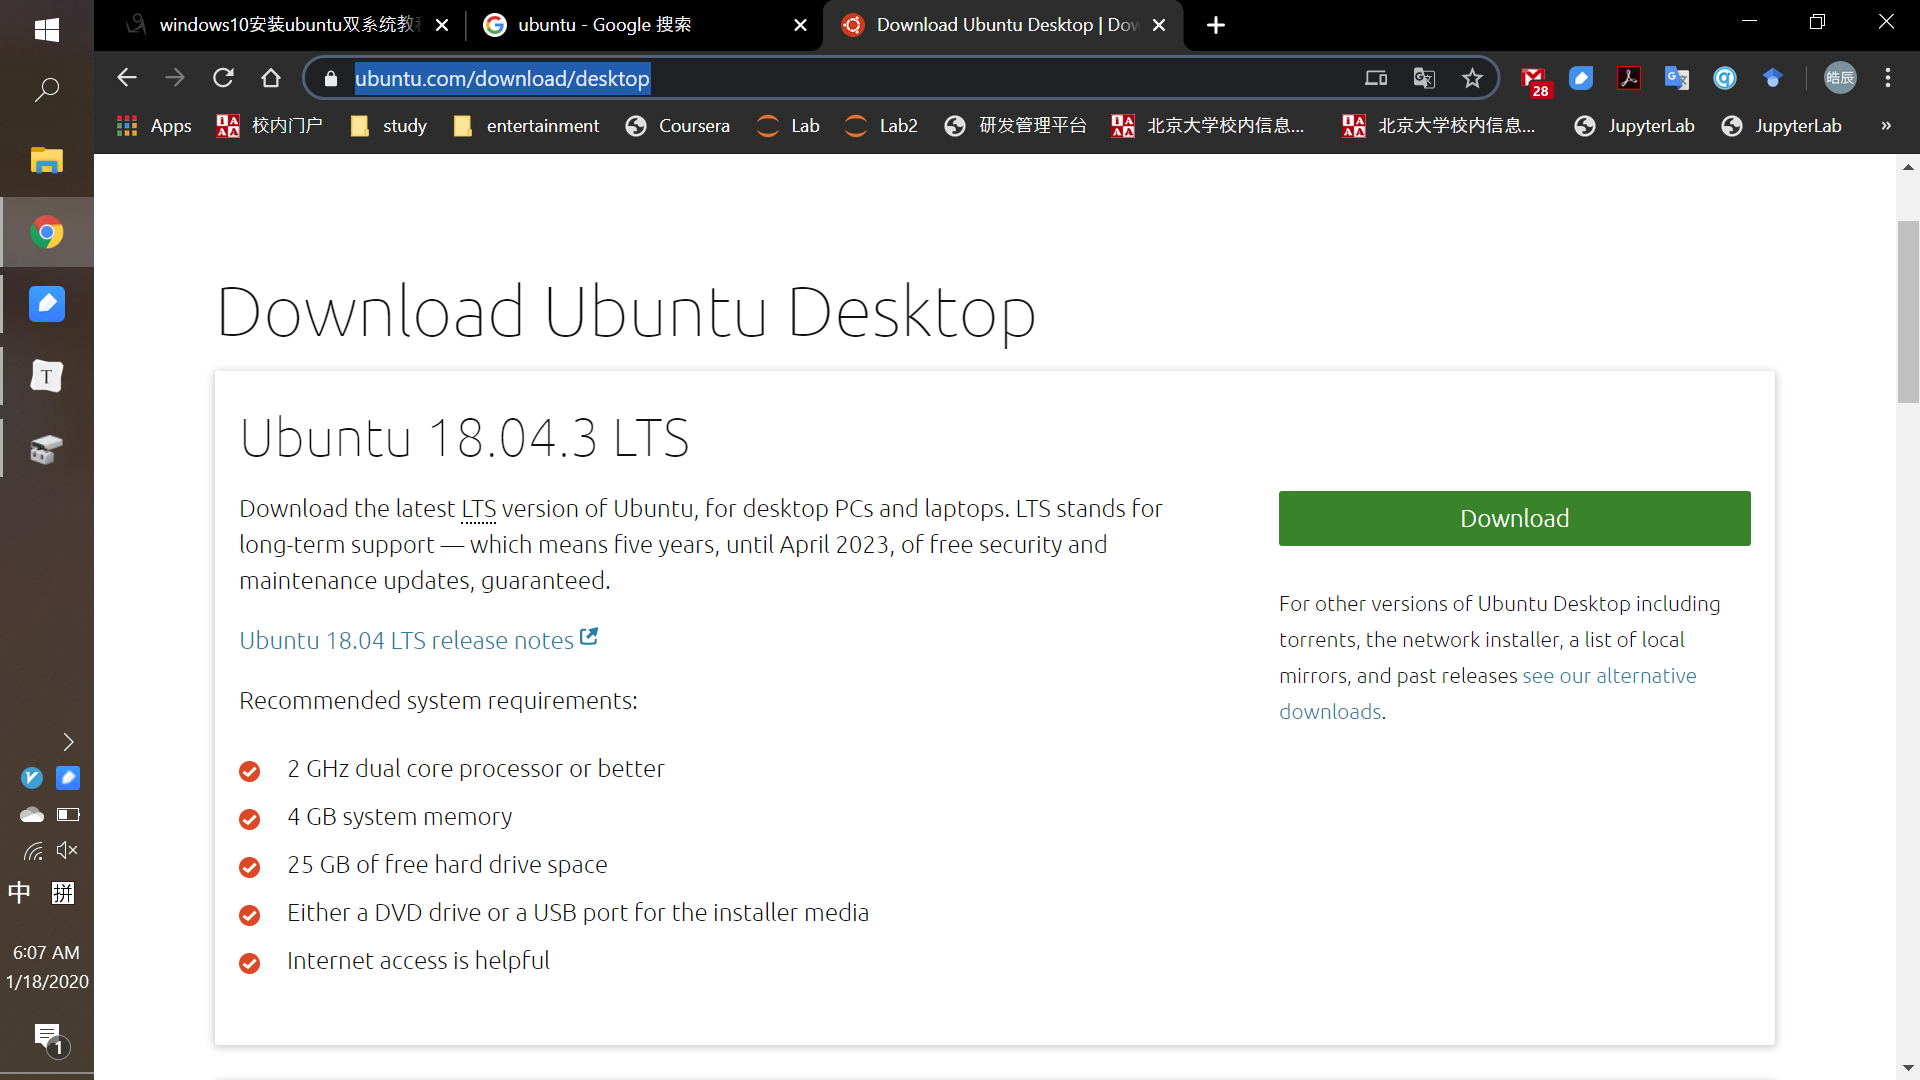
\includegraphics[width=0.7\textwidth]{png/ubuntuDown}
					\caption{Ubuntu 操作系统下载网址。}
					\label{fig:ubuntuDown}
				\end{figure}
			\item [I-c.] 制作启动盘:当系统镜像下载好之后,需要一个新的4G以上的u盘。
				接着下载启动盘制作工具 UltraISO ( \url{https://cn.ultraiso.net/xiazai.html})。
				该软件为免费试用版,下载好之后安装即可(最后一步点击继续试用)。
				接着在 UltraISO 中制作启动盘:
				\begin{itemize}
					\item 打开之前下载的 Ubuntu 镜像文件(文件$\to$打开);
					\item 选择写入硬盘镜像(启动$\to$写入硬盘镜像)。
				\end{itemize}
				注意写入过程中会格式化u盘。
			 	\begin{figure}[htbp]
			 		\centering
			 		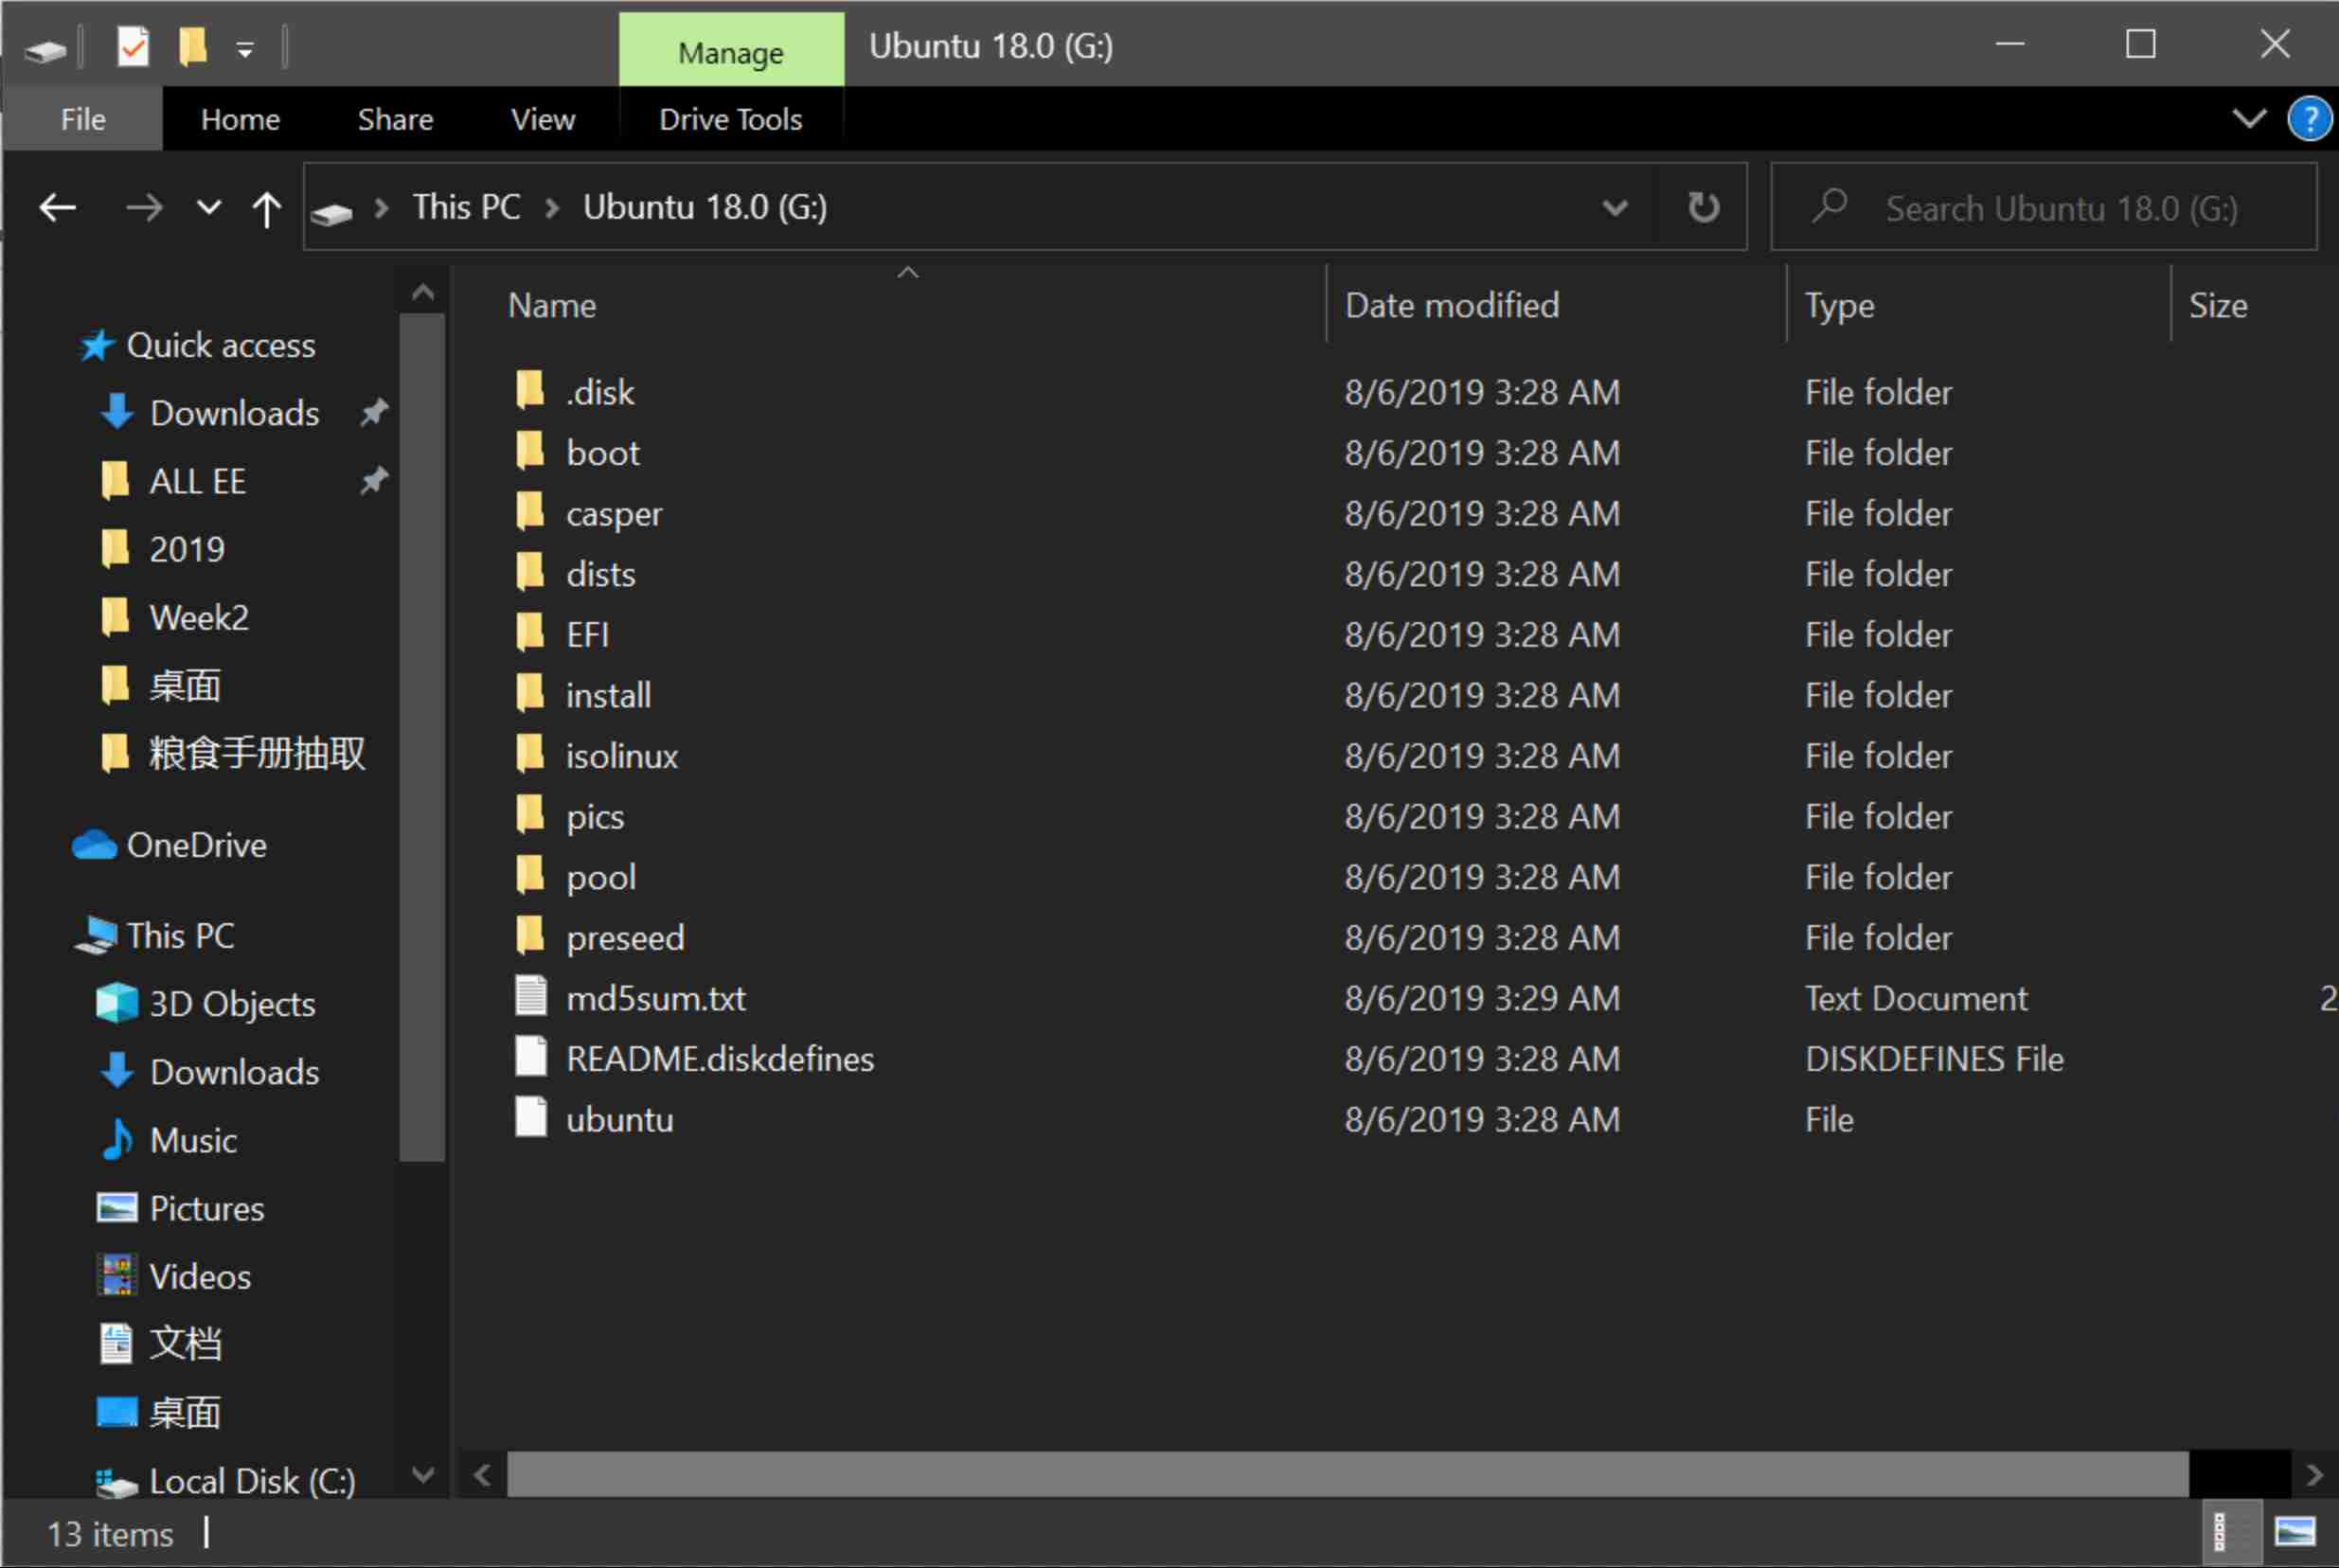
\includegraphics[width=0.75\textwidth]{png/UltraISO}
			 		\caption{制作完成后的启动盘。}
			 		\label{fig:UltraISO}
			 	\end{figure}
		\end{itemize}

	\item [II.] 安装工作
	        \begin{itemize}
                        \item [II-a.] 安装前的准备工作:
                                \begin{itemize}
                                        \item 在BIOS中关闭BOOT SAFTY MODE(或类似的名称),即所谓的安全模式。这个其实会阻止任何非Windows认证的系统启动。 
                                        \item 检查你的机器是否存在Optane分区。Optane内存(傲腾)是Intel的一项技术,在19年以后的计算机中可能会出现。
                                          它会对硬盘做快速缓存,一个副作用是导致你对硬盘的手工修改失效,包括ubuntu安装程序,如果有,务必在安装前关闭。
                                          安装成功之后,可以再打开。
 				                  \begin{figure}[htbp]
					                  \centering
						          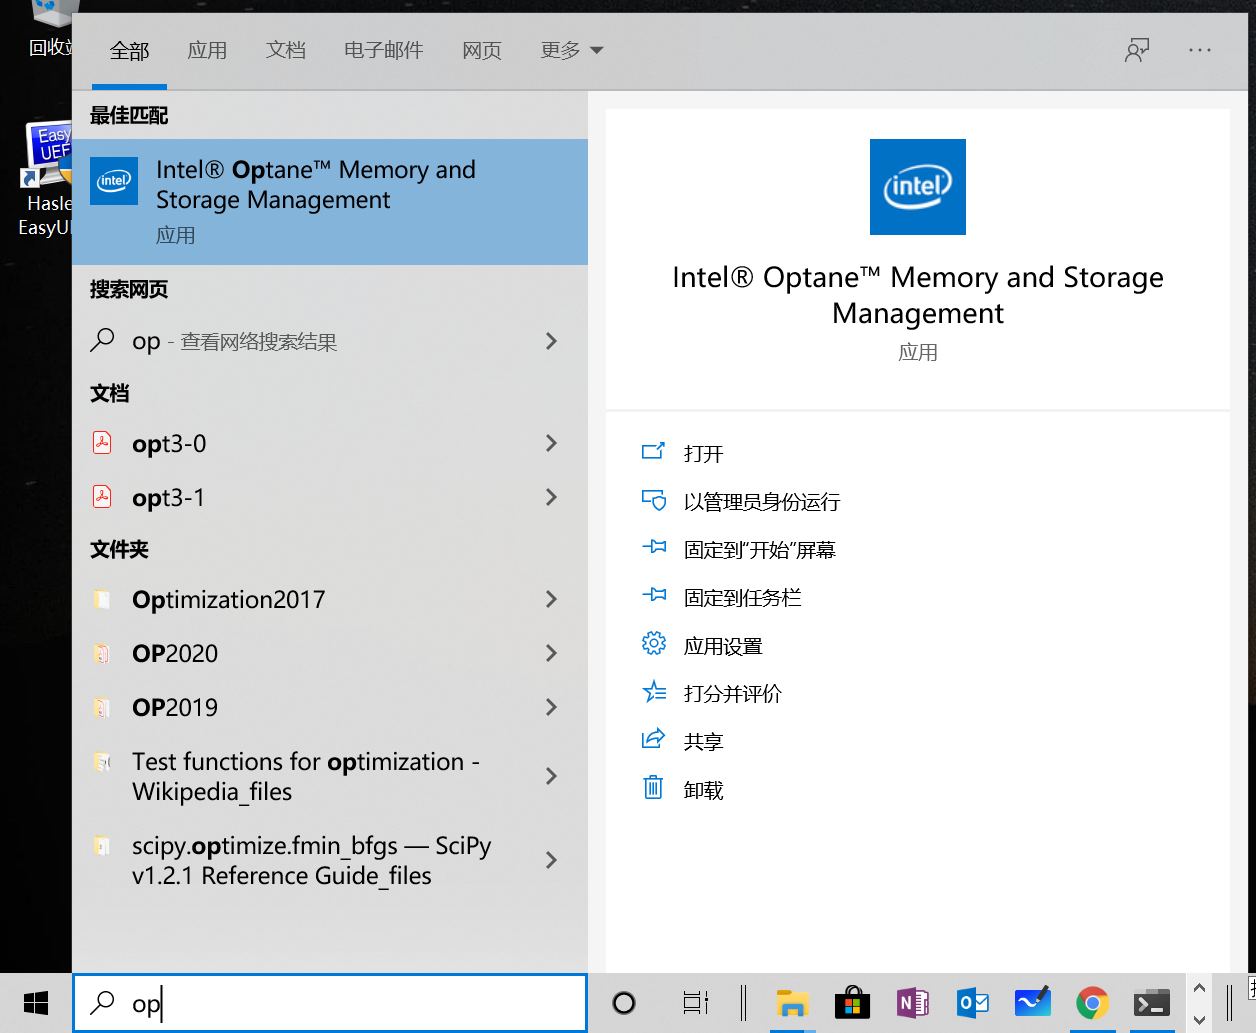
\includegraphics[width=0.75\textwidth]{png/optane}
                                                          \caption{检查Optane。}
                                                          \label{fig:optane}
				                  \end{figure}
                                \end{itemize}
			\item [II-b.] 关闭所有程序后,插入制作好的启动盘,重新启动电脑,
				并且在启动出现提示时按 F12(不同电脑不同)键进入 boot 选项,
				选择对应的启动盘作为启动介质(将 USB 移动到最上面),
				然后按 F10 保存并退出,接着选择安装 Ubuntu。
				\begin{figure}[htbp]
					\centering
					\subfigure[将启动盘作为首选启动项]{
						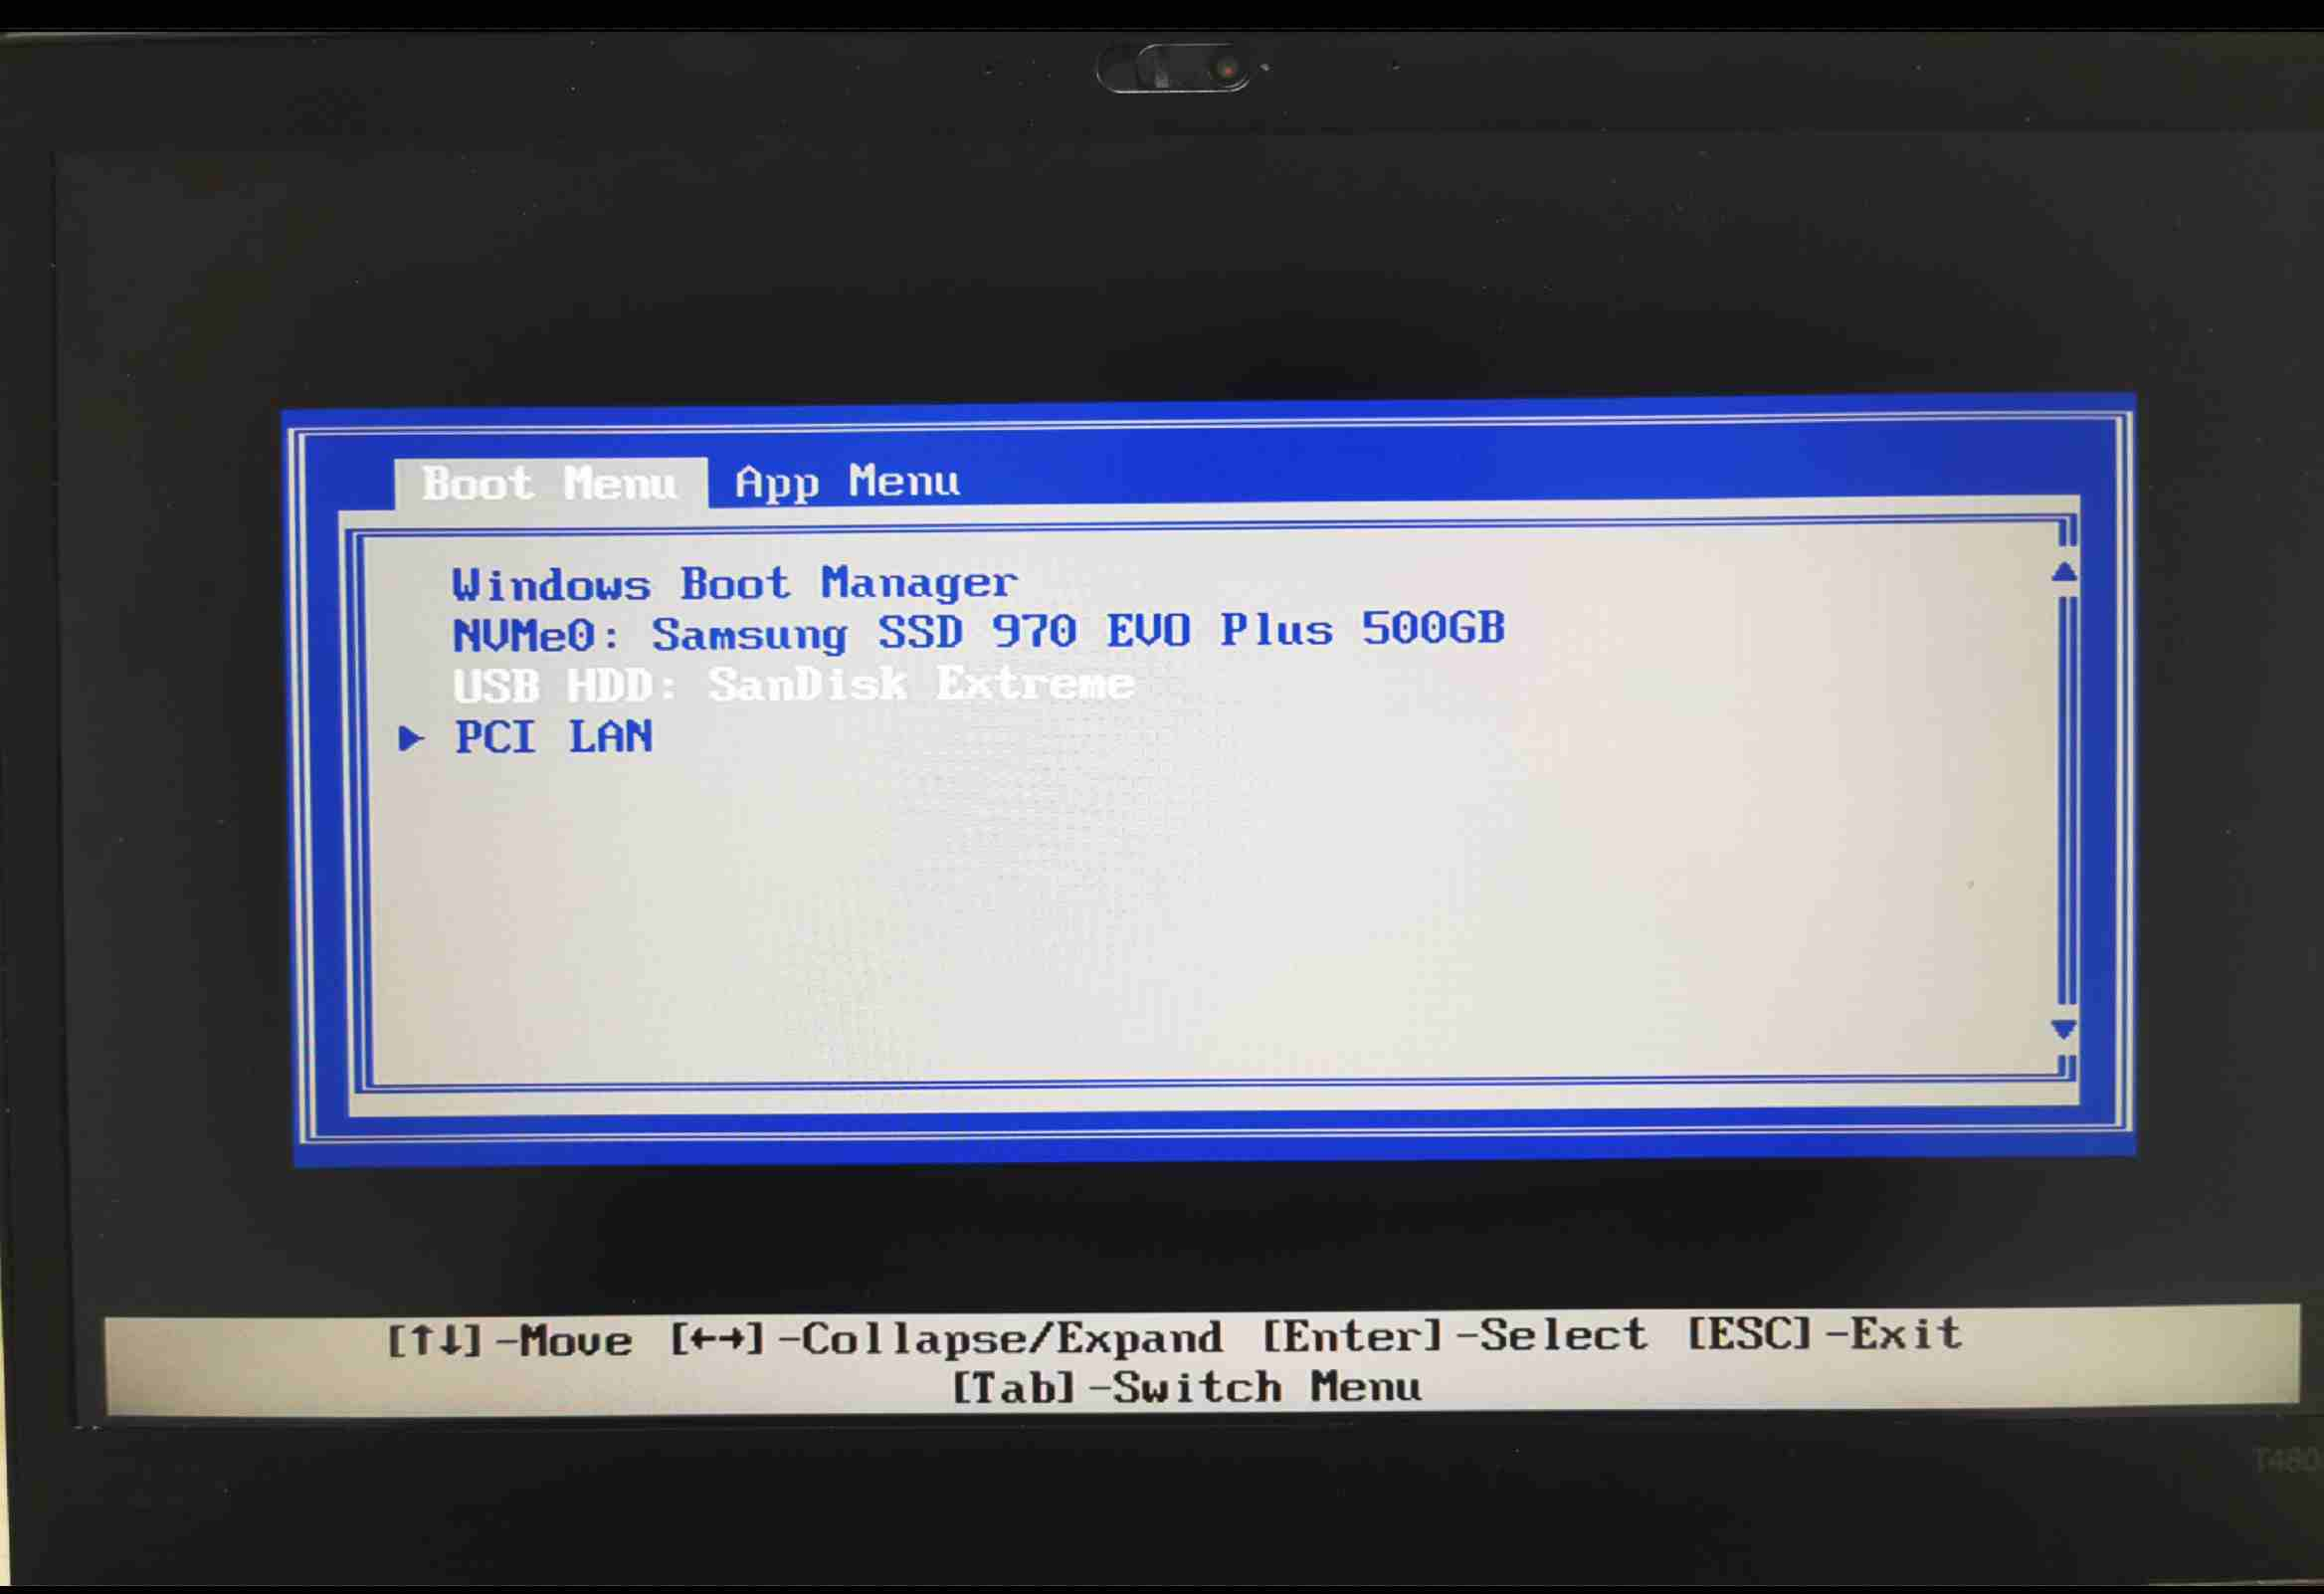
\includegraphics[width=0.42\linewidth]{png/bootMenu}
					}
					\hfill
					\subfigure[选择安装Ubuntu]{
						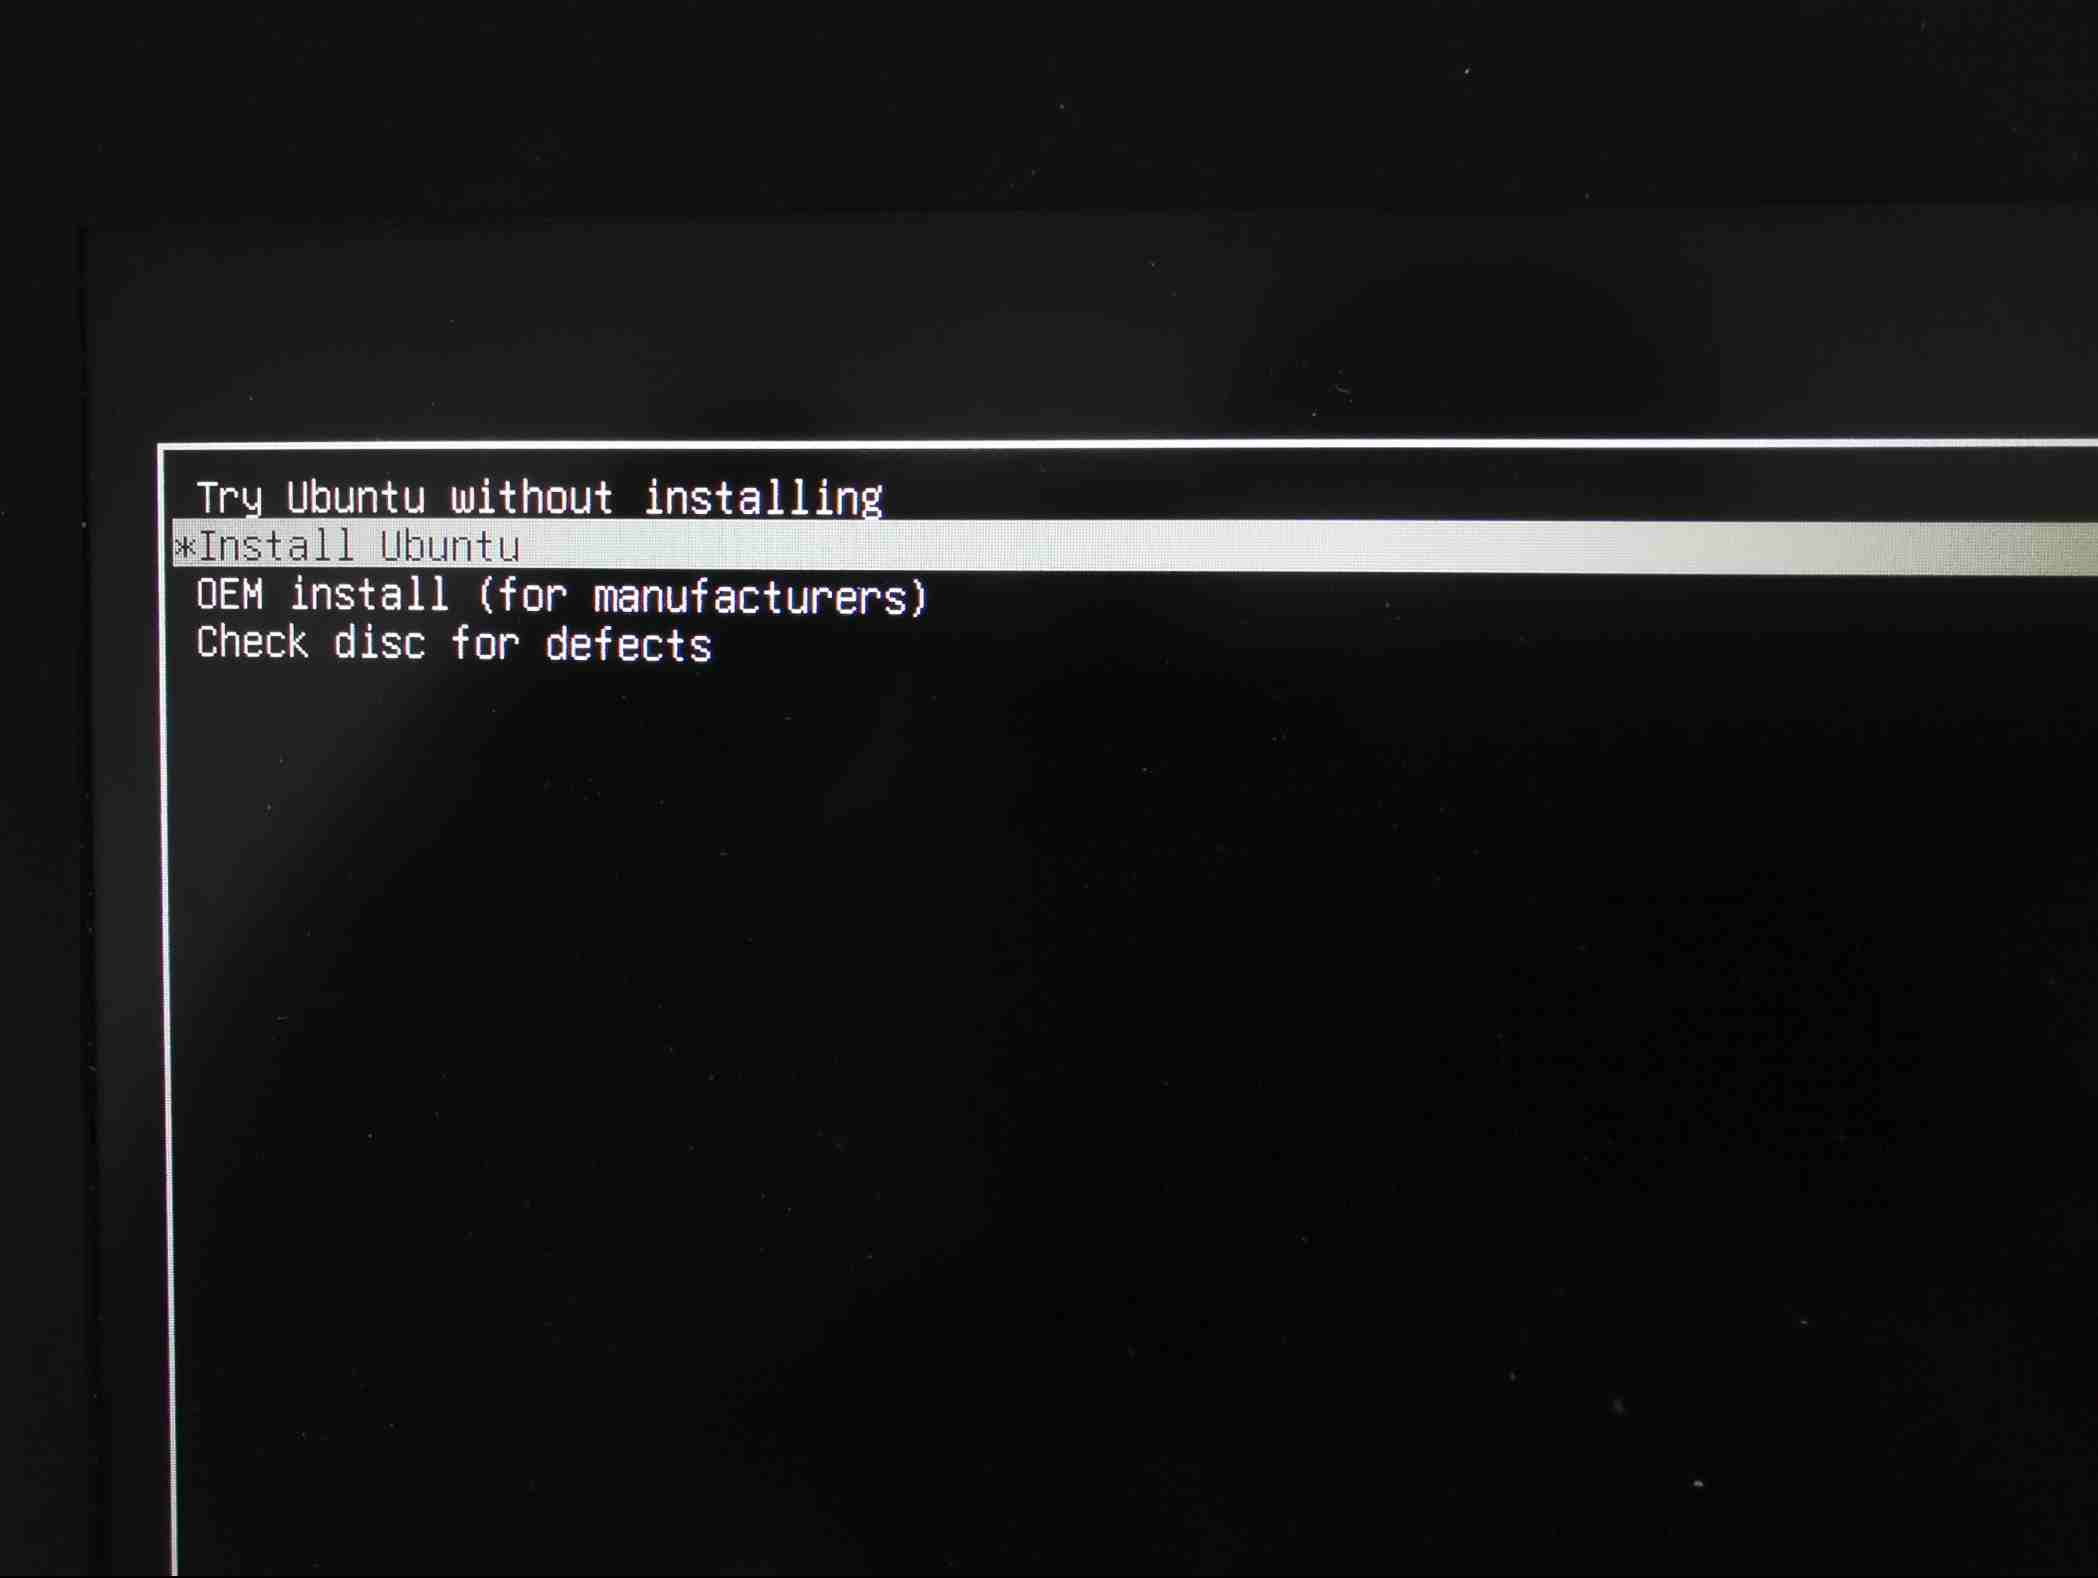
\includegraphics[width=0.42\linewidth]{png/InstallUbuntu}
					}
					\label{fig:UbuntuInstall}
				\end{figure}
			
				如果没有直接进入到 boot 选项的快捷键,可先进入 bios 界面,
				然后切换到 boot 选项进行设置,
				不同型号不同品牌的电脑可能会稍有差异。
			\item [II-c.] 接着选择合适的语言和键盘布局,正常安装、一路下一步后直到安装类型界面,
				此时选择其他选项进入系统分区,选中之前压缩磁盘得到的空闲硬盘空间,
				选择左下角的 + 号依次添加四个分区:
				\begin{itemize}
					\item 系统分区,即存放Ubuntu系统的分区
					(大小20GB,主分区,空间起始位置,Ext4文件系统,挂载点/);
					\item 交换分区,即内存交换空间,一般和本机内存大小相同
					(大小16GB,逻辑分区,空间起始位置,交换空间);
					\item boot分区,即启动文件分区
					(大小200M/400M,逻辑分区,空间起始位置,Ext4文件系统,挂载点/boot);
					\item 用户分区,即真正使用的剩余空间,将空余的硬盘全部分配
					(大小为剩下全部,逻辑分区,空间起始位置,Ext4文件系统,挂载点/home)。
				\end{itemize}
				\begin{figure}[htbp]
					\centering
					\subfigure[语言键盘设置]{
						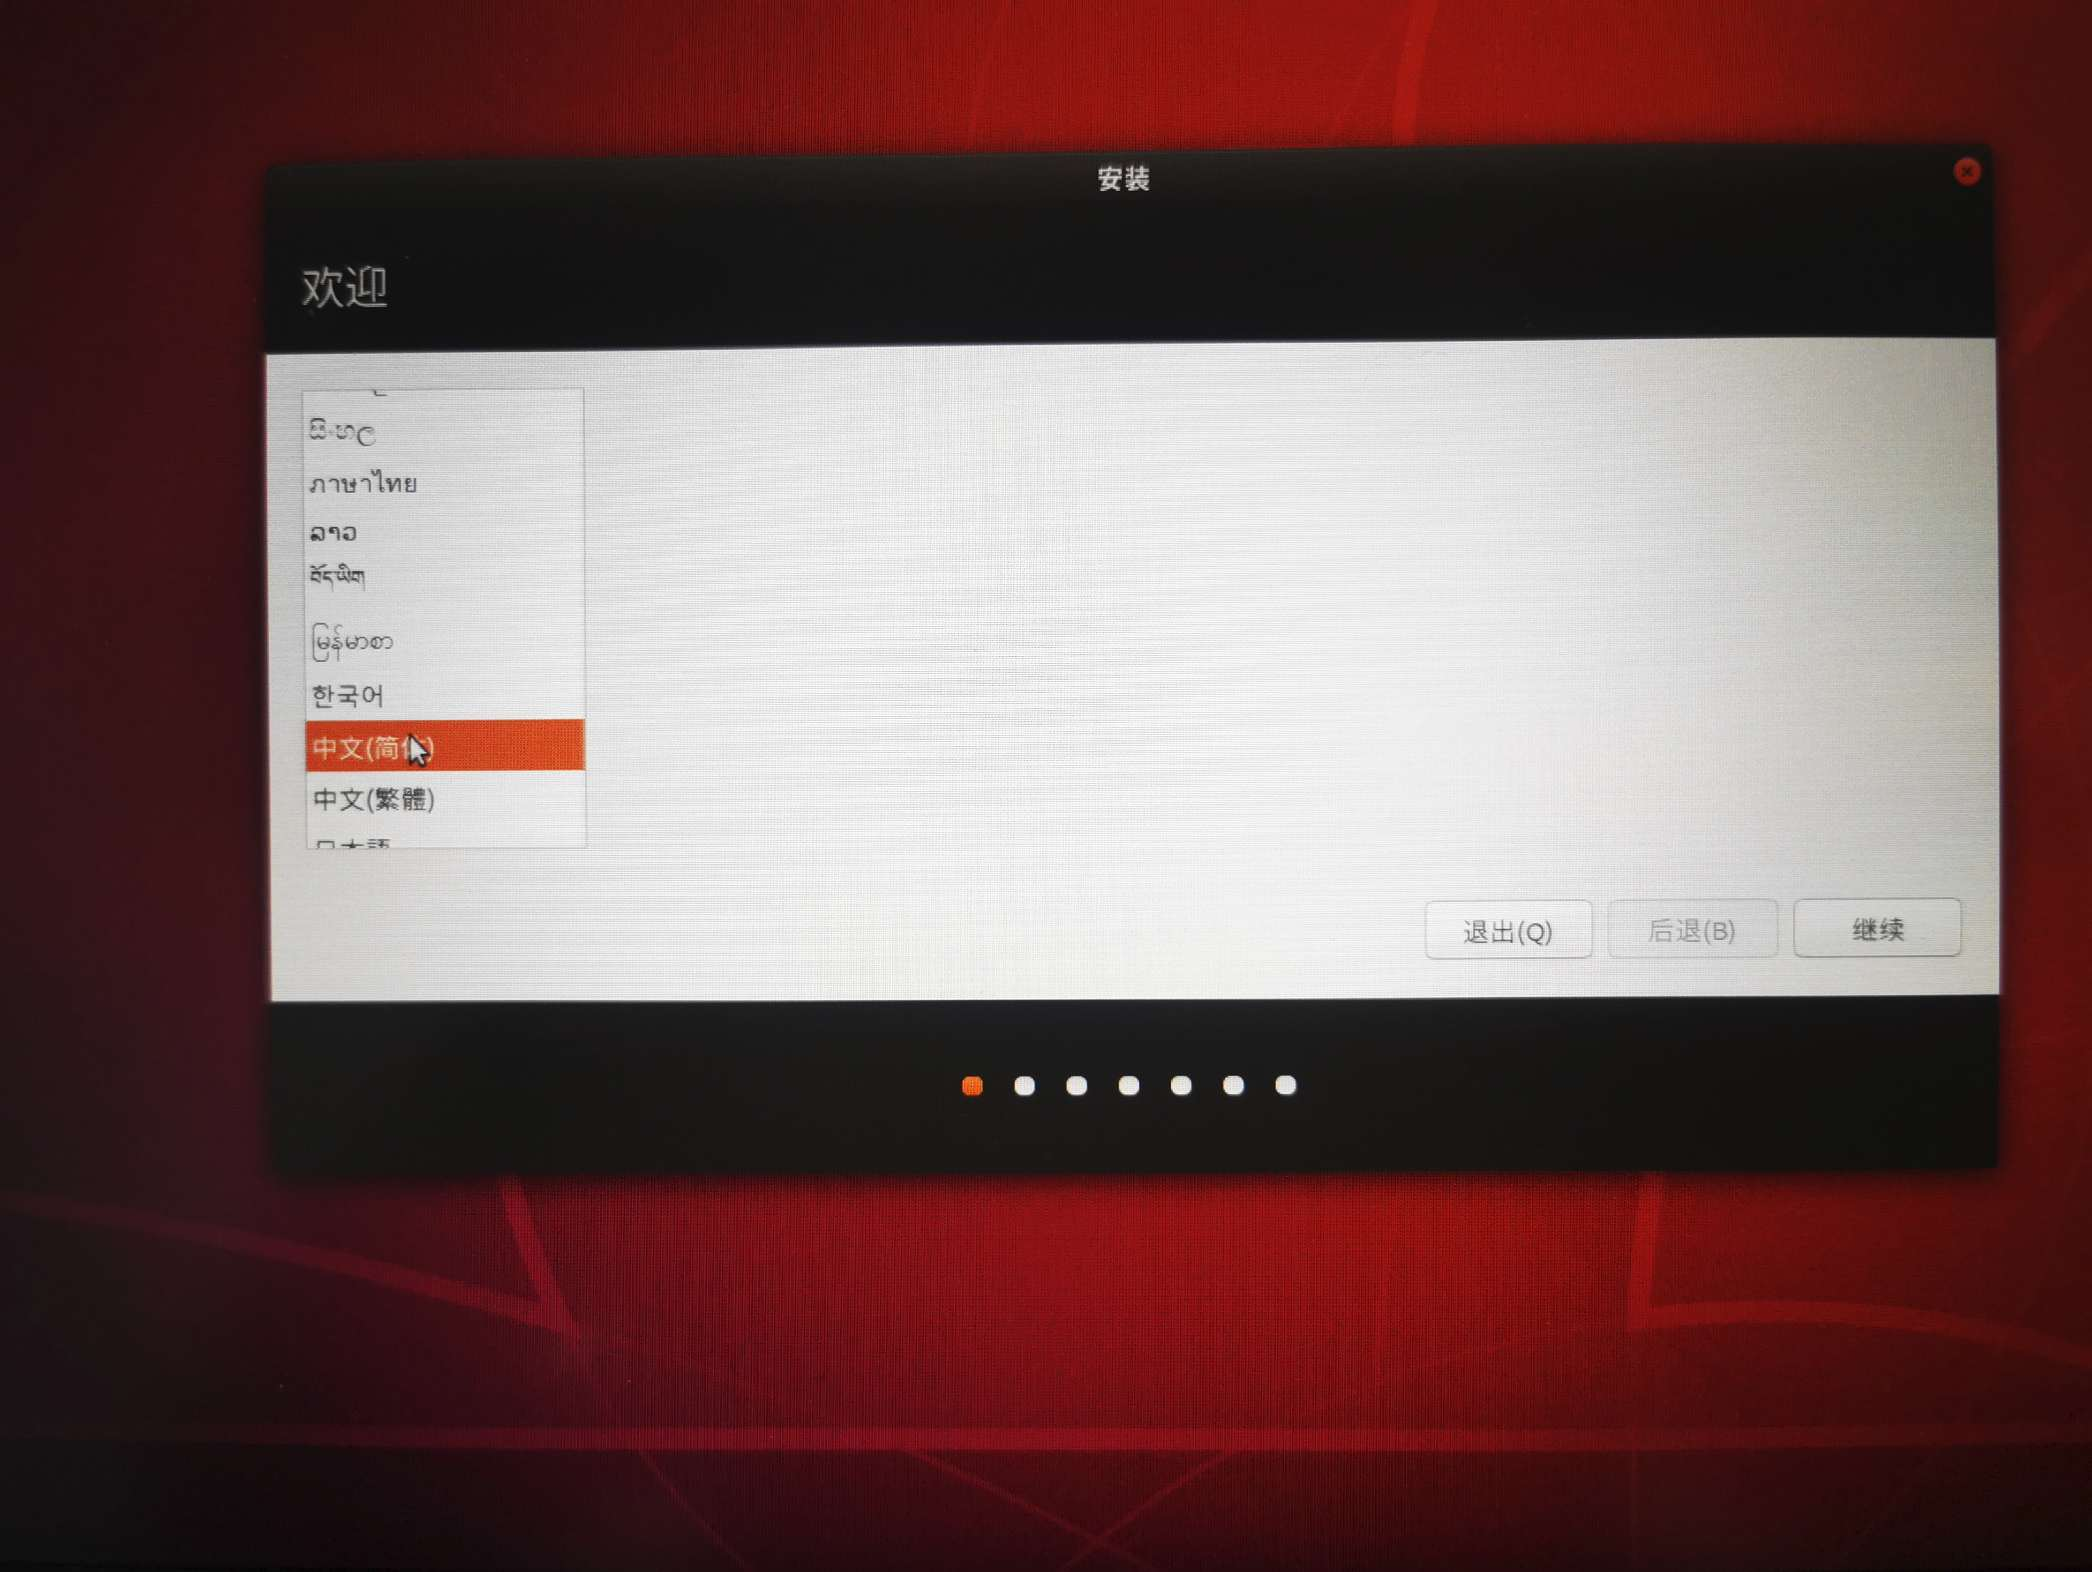
\includegraphics[width=0.42\linewidth]{png/language}
					}
					\hfill
					\subfigure[安装类型]{
						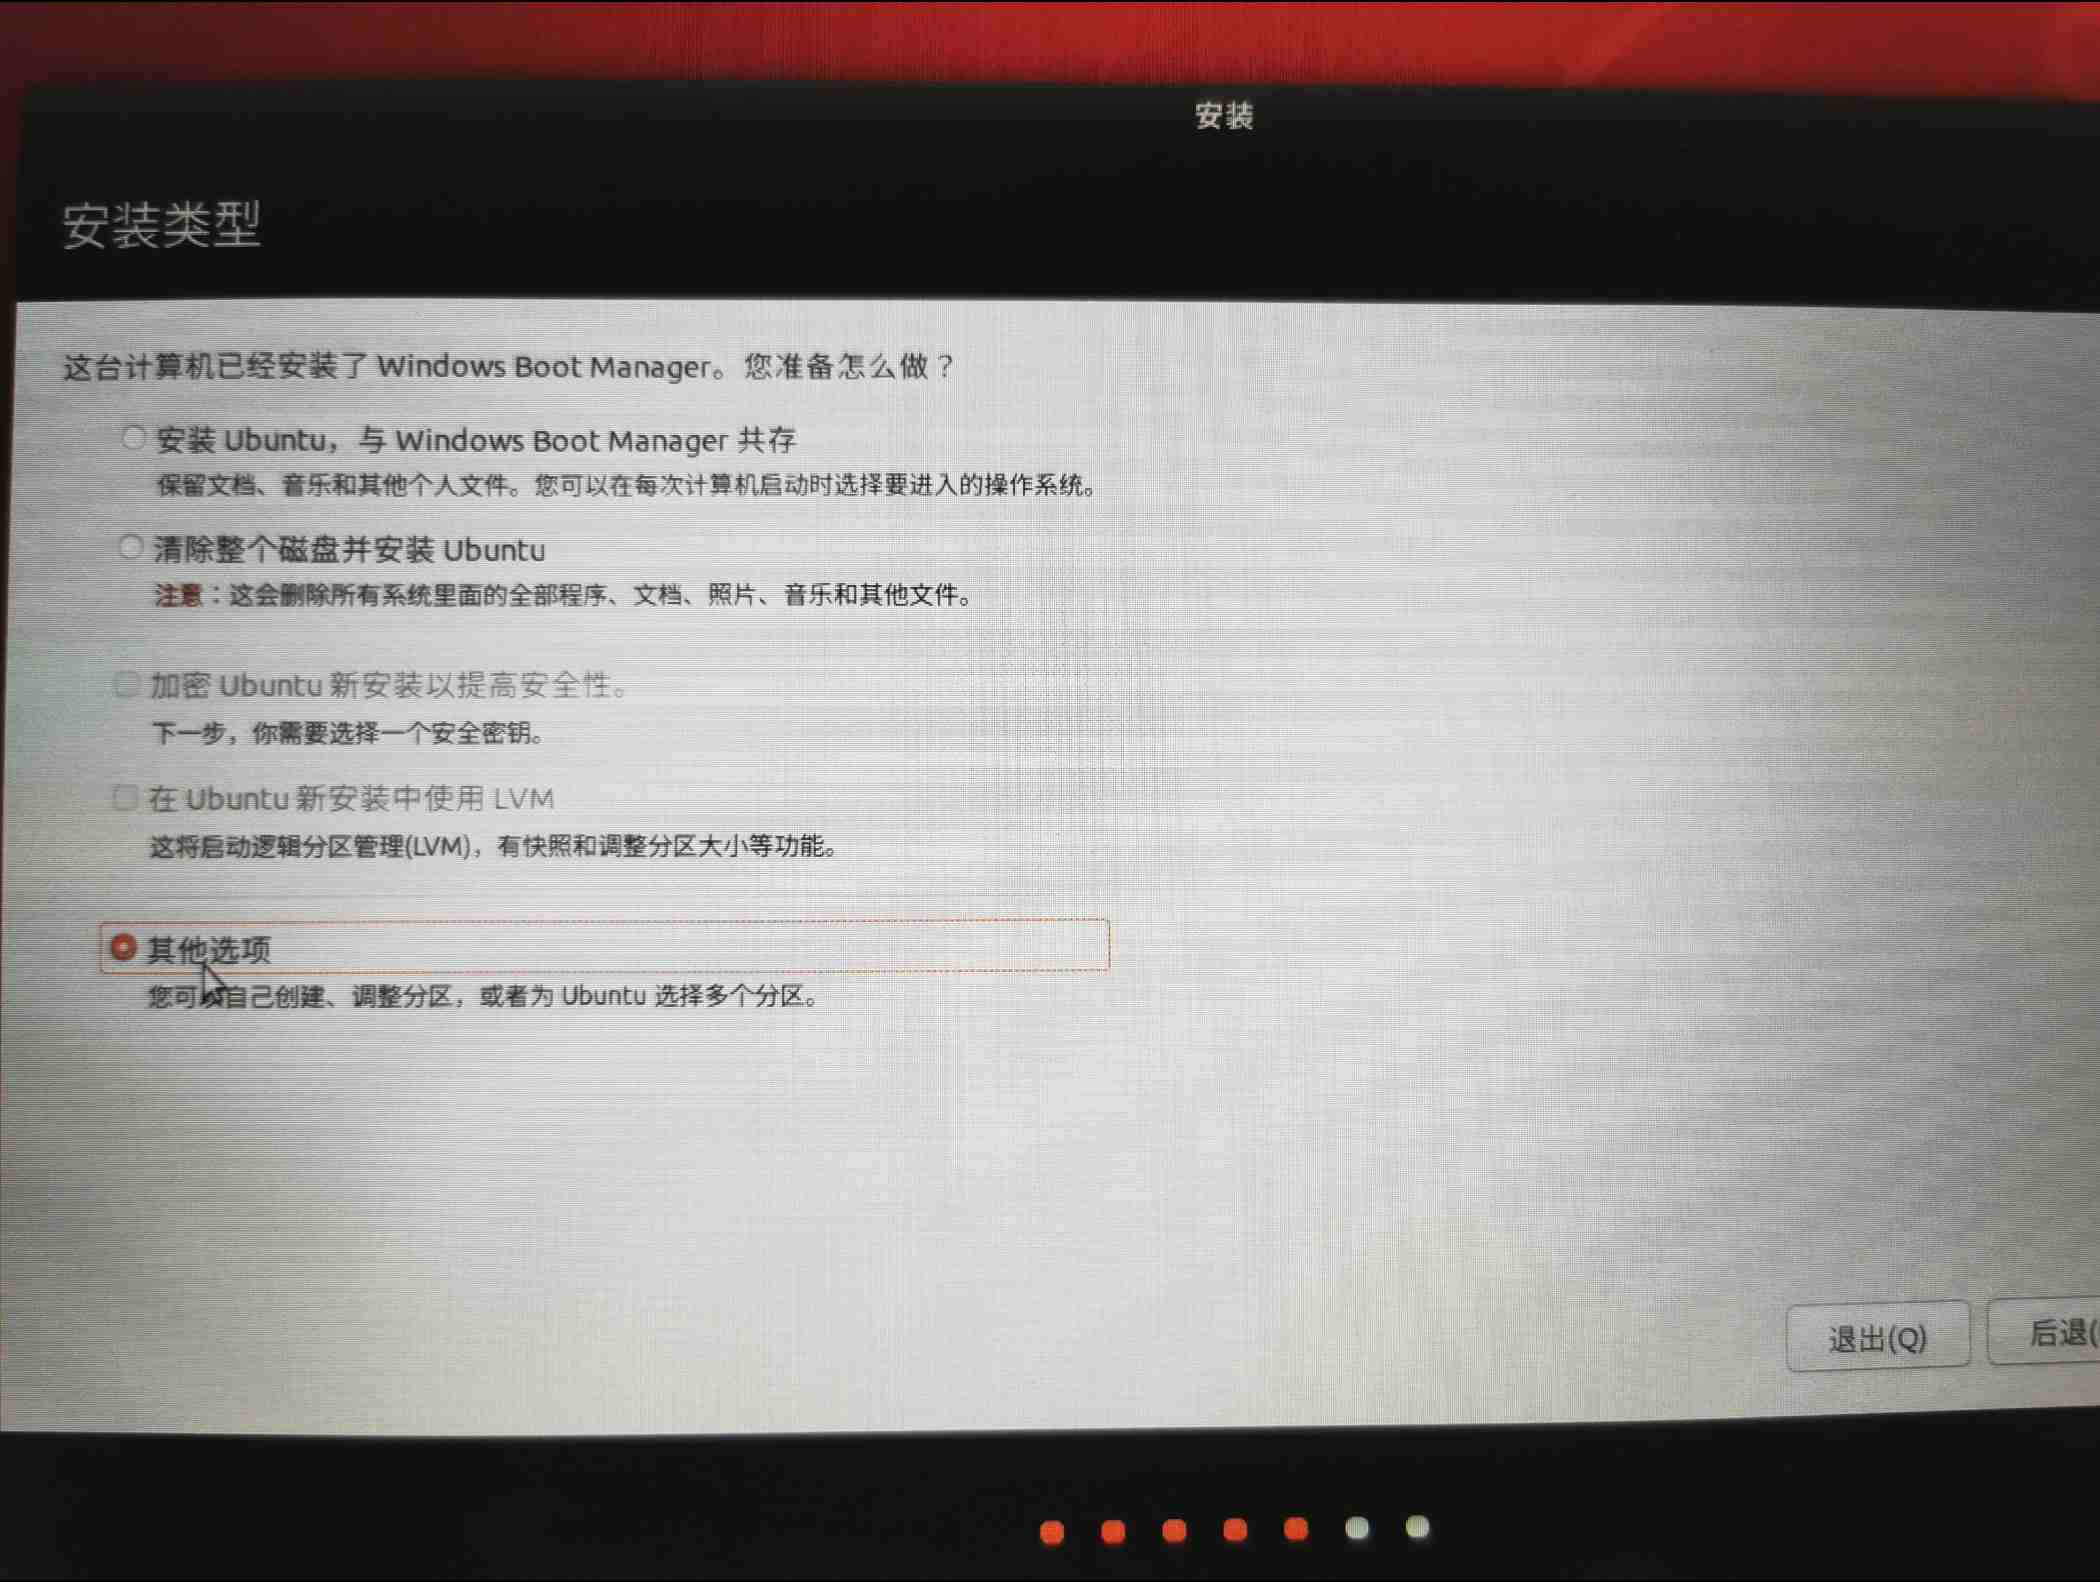
\includegraphics[width=0.42\linewidth]{png/InstallType}
					}
					\label{fig:installType}
  				\end{figure}
				\begin{figure}[htbp]
					\centering
					\subfigure[系统分区设置]{
						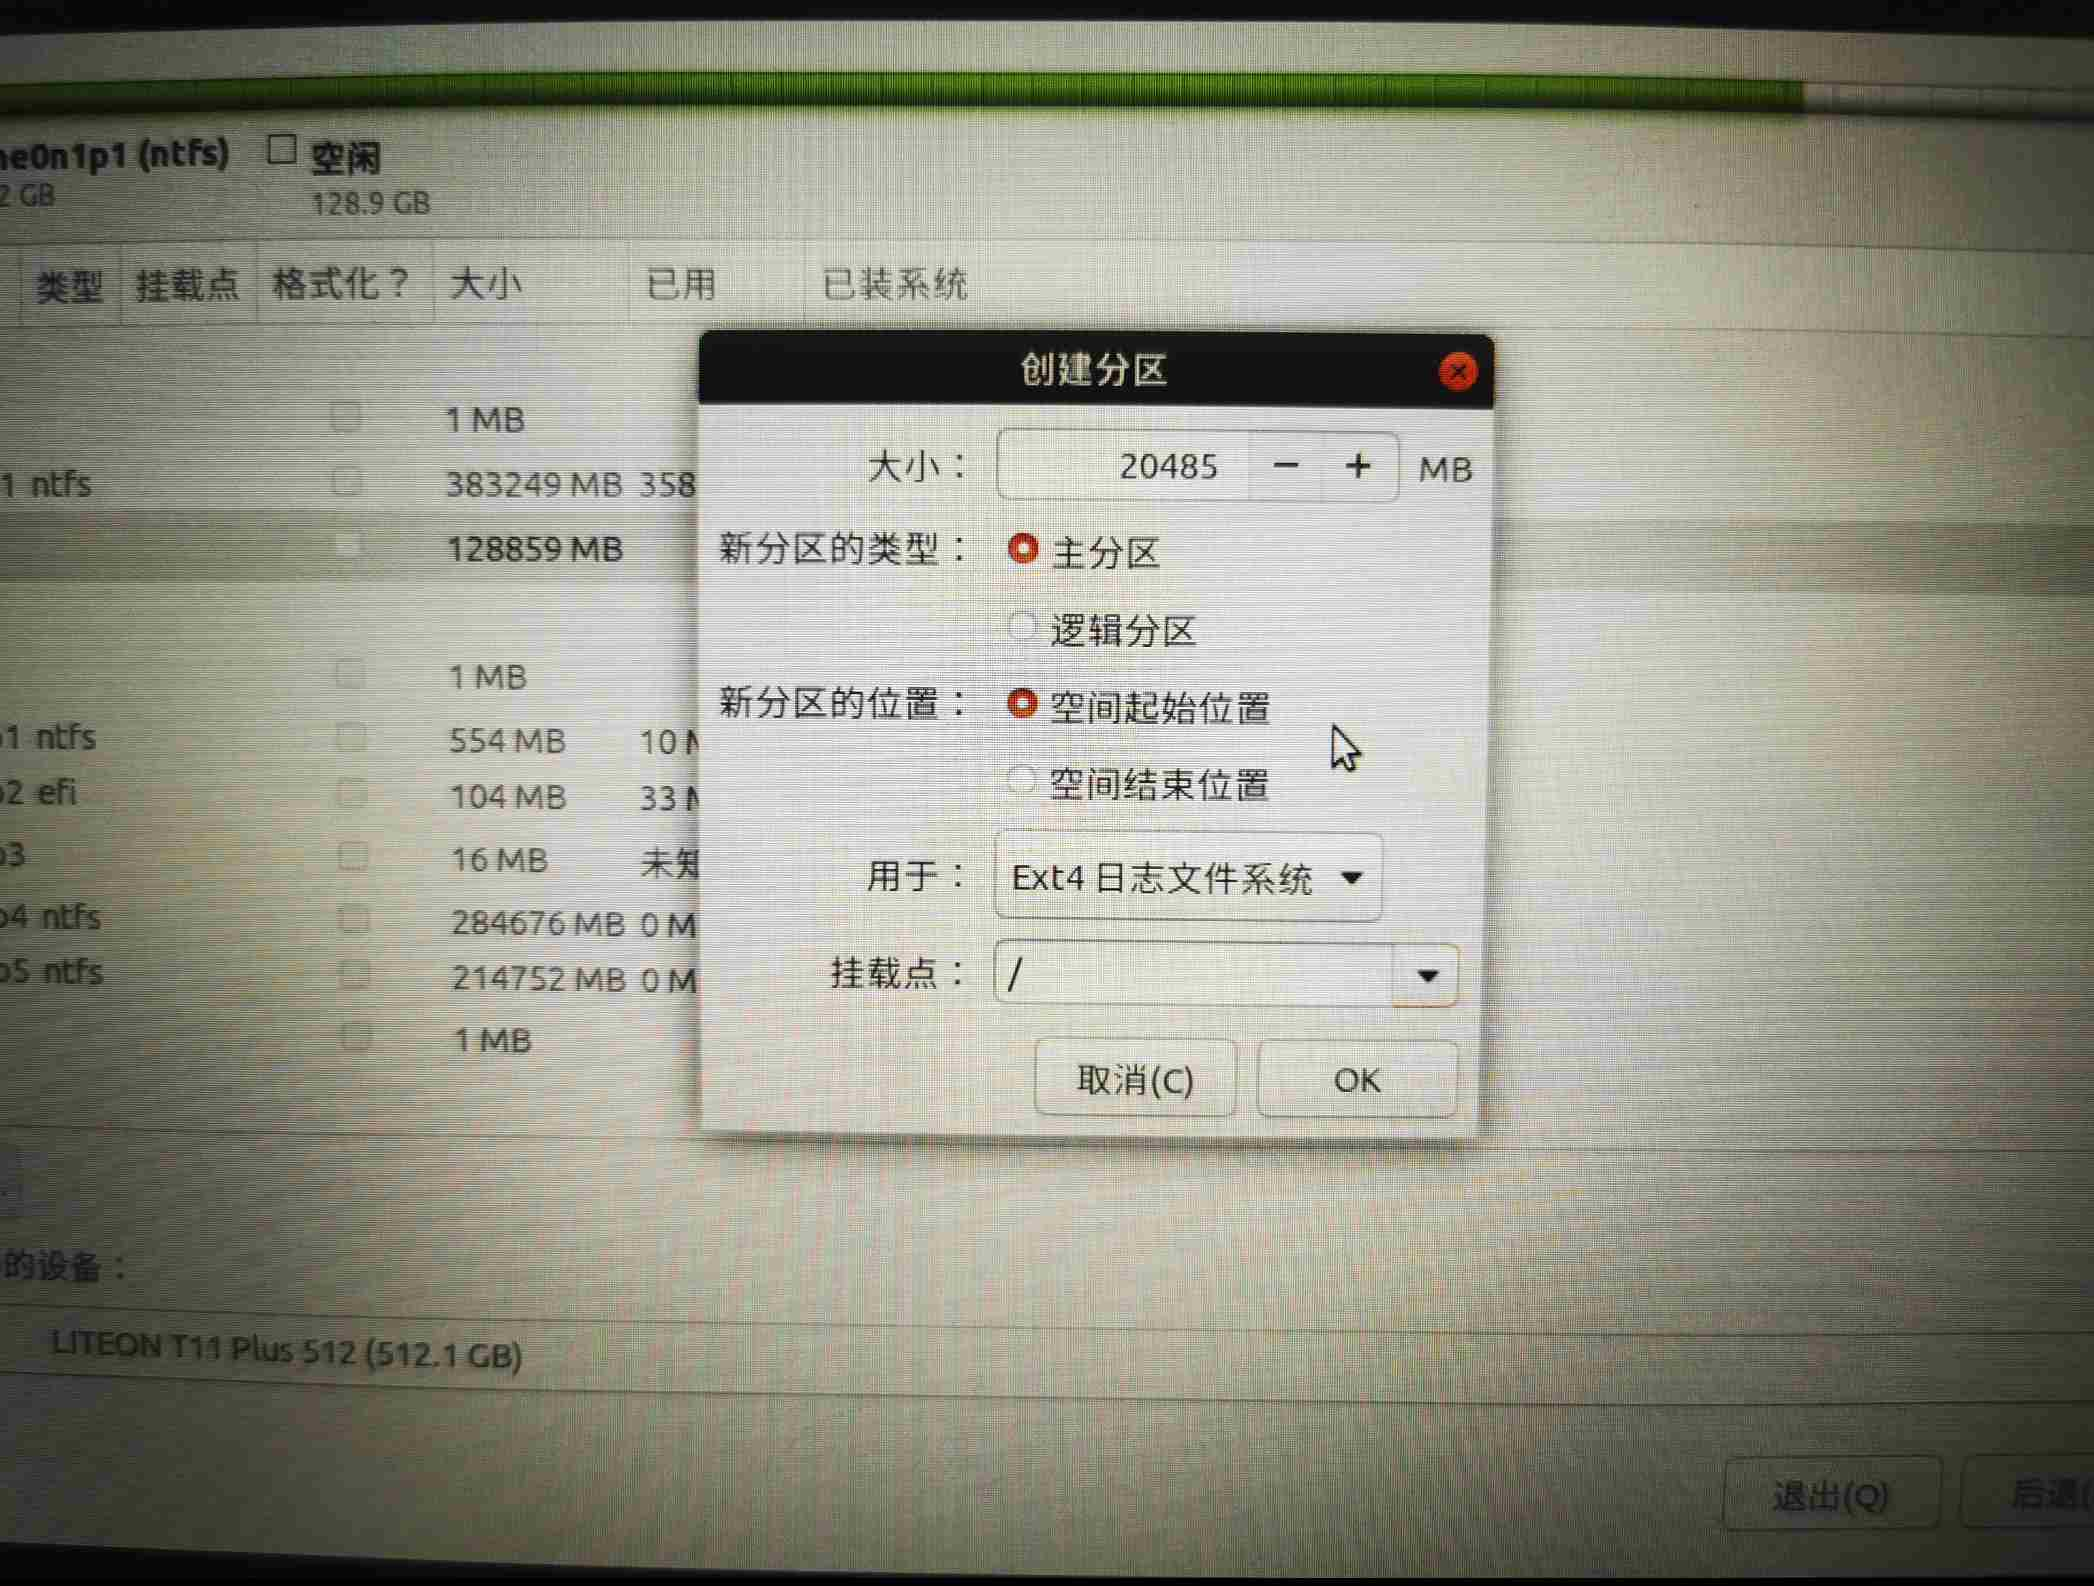
\includegraphics[width=0.45\linewidth]{png/system}
					}
					\hfill
					\subfigure[交换分区设置]{
						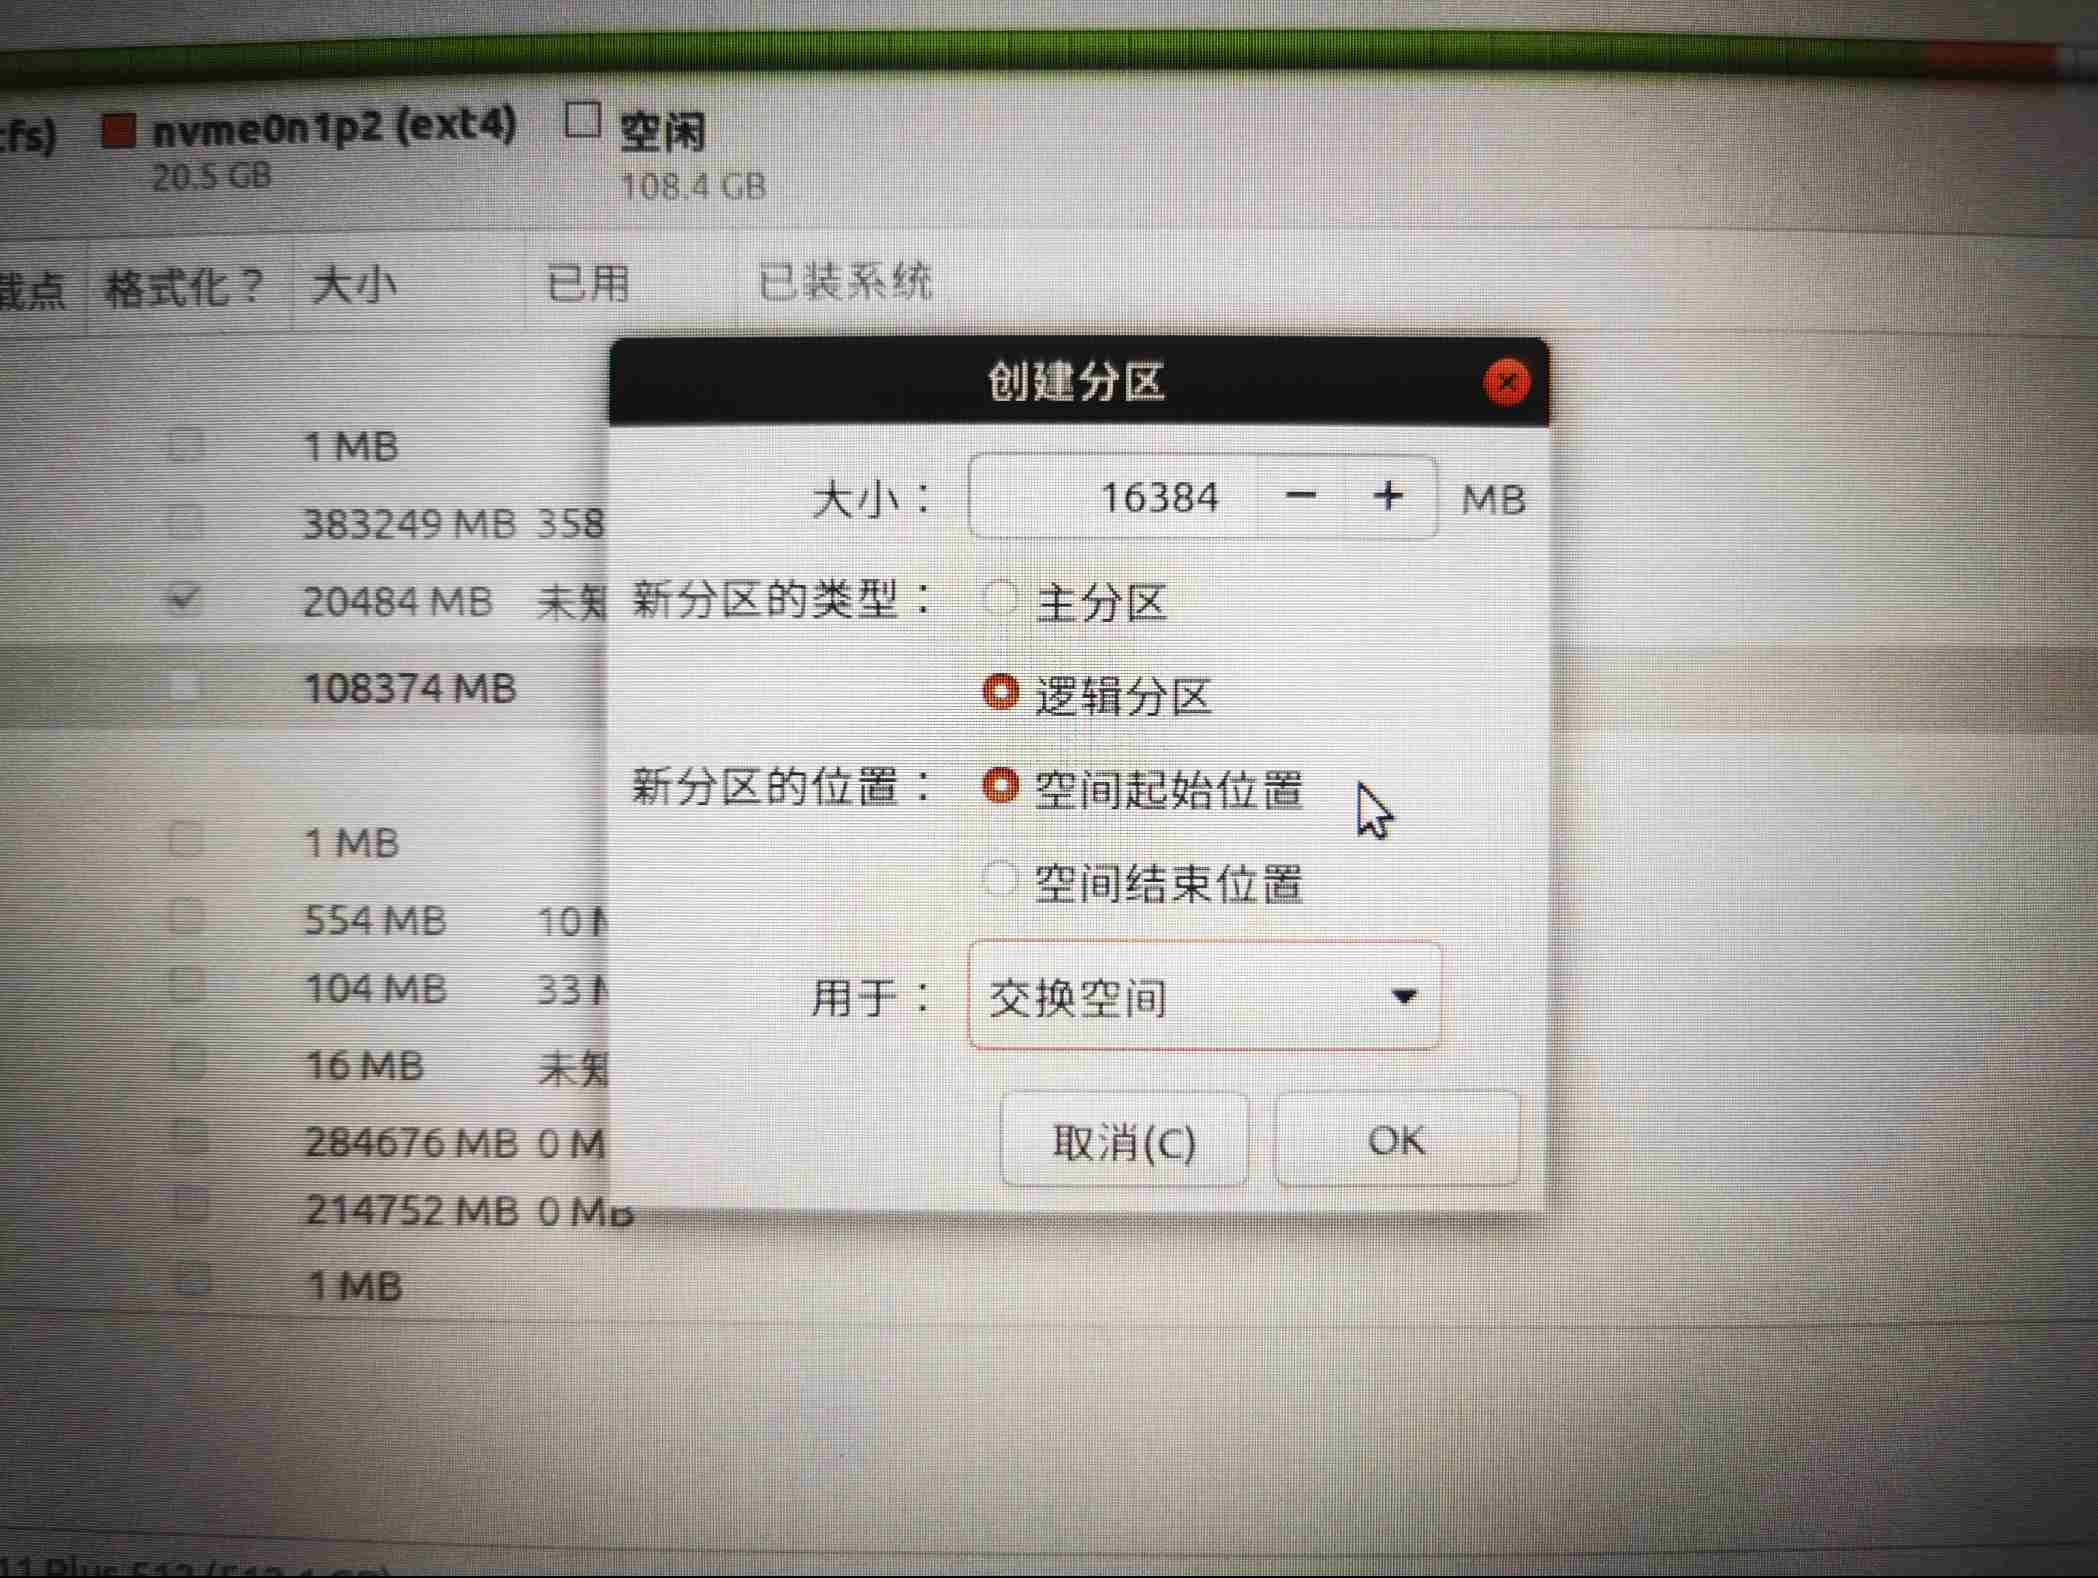
\includegraphics[width=0.45\linewidth]{png/swap}
					}
					\hfill
					\subfigure[boot分区设置]{
						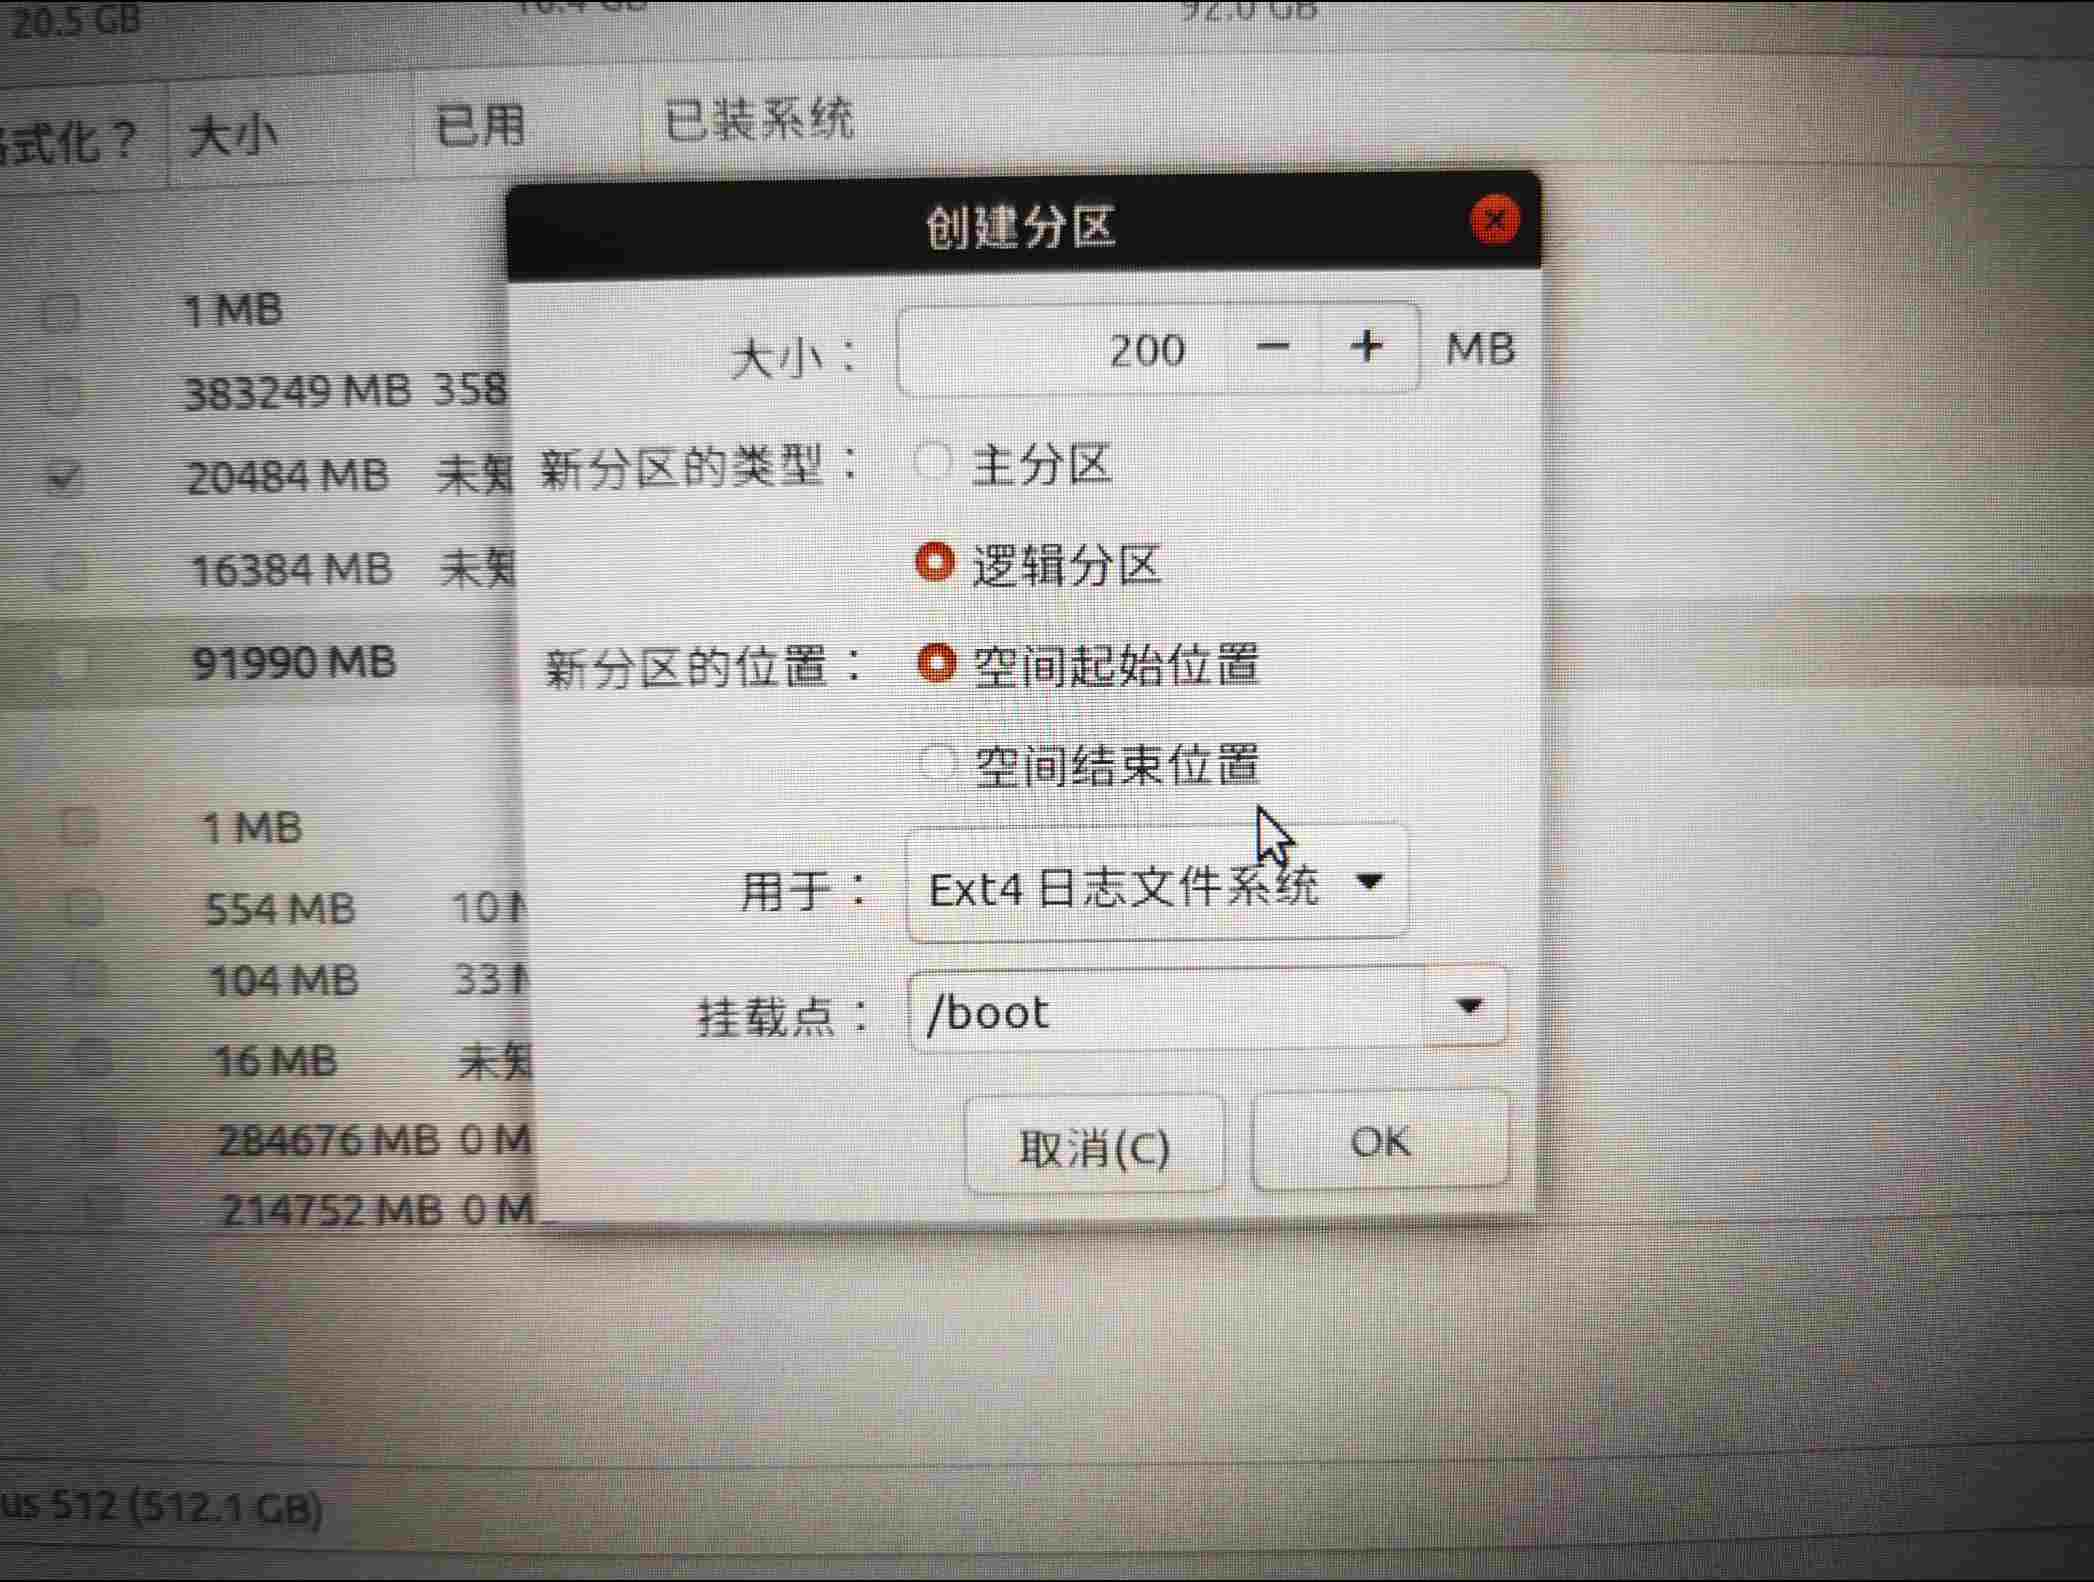
\includegraphics[width=0.45\linewidth]{png/boot}
					}
					\hfill
					\subfigure[用户分区设置]{
						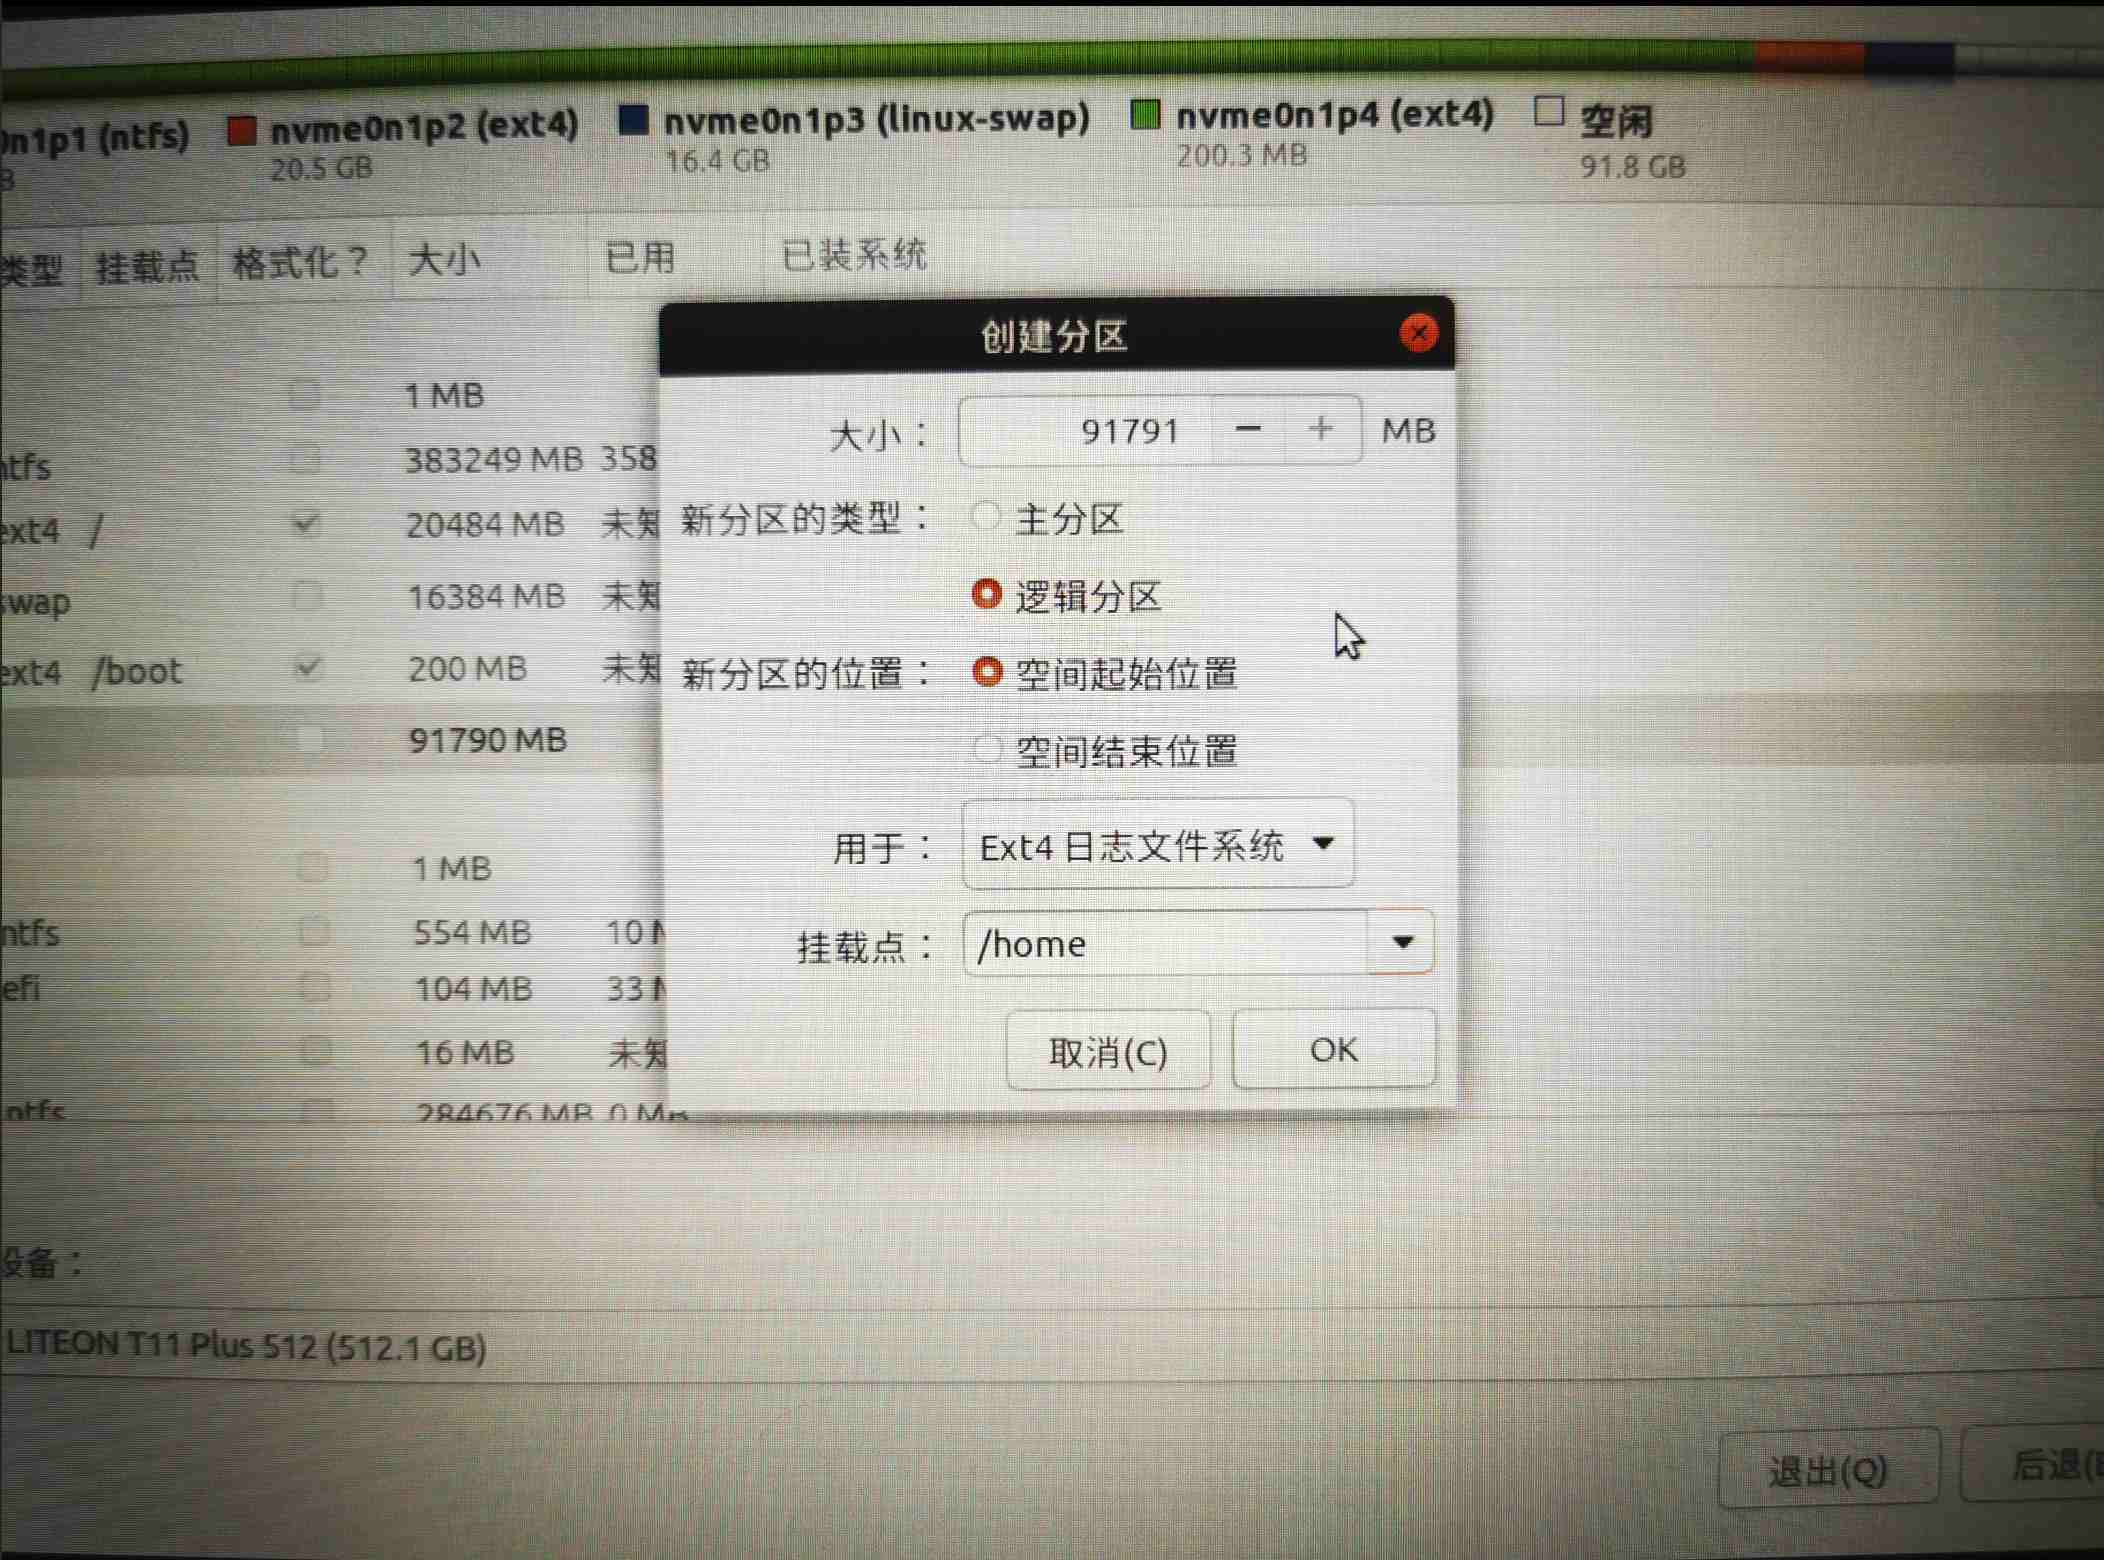
\includegraphics[width=0.45\linewidth]{png/user}
					}
				    \hfill
				    \subfigure[分区完成]{
				    	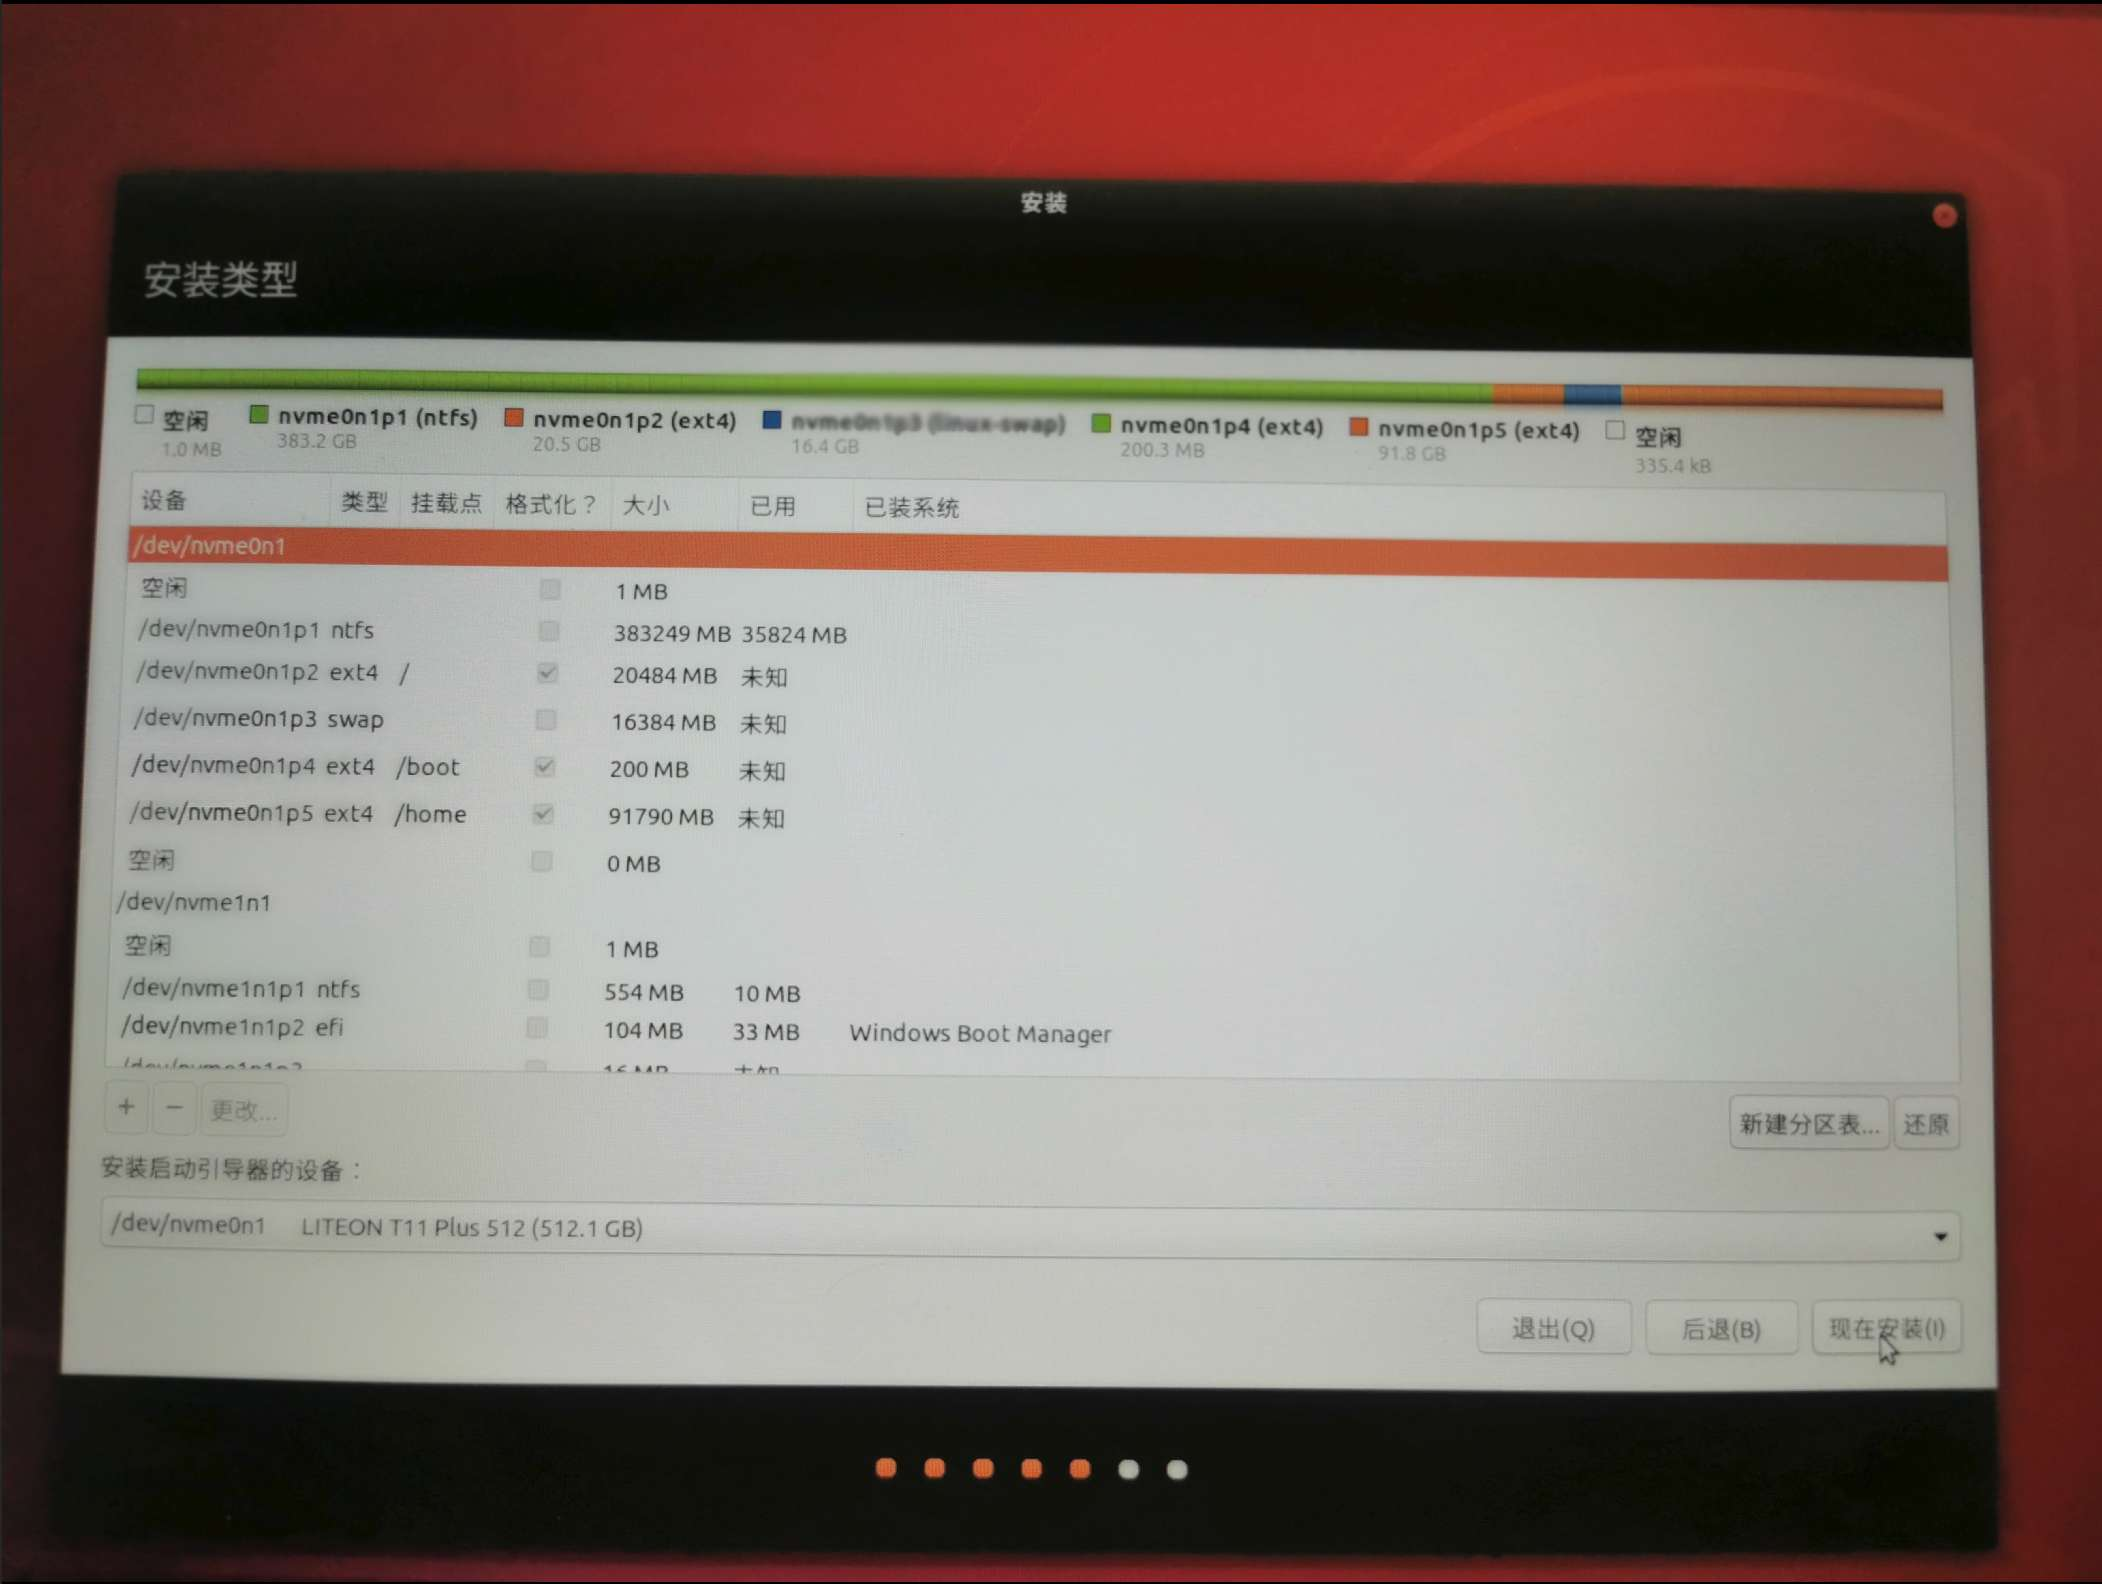
\includegraphics[width=0.8\linewidth]{png/allocated}
				    }
					\label{fig:setting}
				\end{figure}
			\item [II-d.] 分配之后的分区表会出现 4 个未知的新分区,然后点击继续安装。
				选择时区和用户名密码,自行设置后等待安装完成。
		\end{itemize}
	\item [III.] 启动问题
		\begin{itemize}
                        \item [III-a.] 检查你的efi启动分区内容是否正确。这个需要一定专业硬件知识。建议大家下载easyuefi软件完成。运行之后,
                          在下图中必须确保ubuntu启动项在第一位。如果不是,用绿色的上箭头修改启动顺序。注意对存在Optane的机器,当你每次重新激活Optane时,
                          都会将Windows Boot Manager移动到第一位,必须在激活重启之后重新调整efi。  
				\begin{figure}[htbp]
					\centering
			 		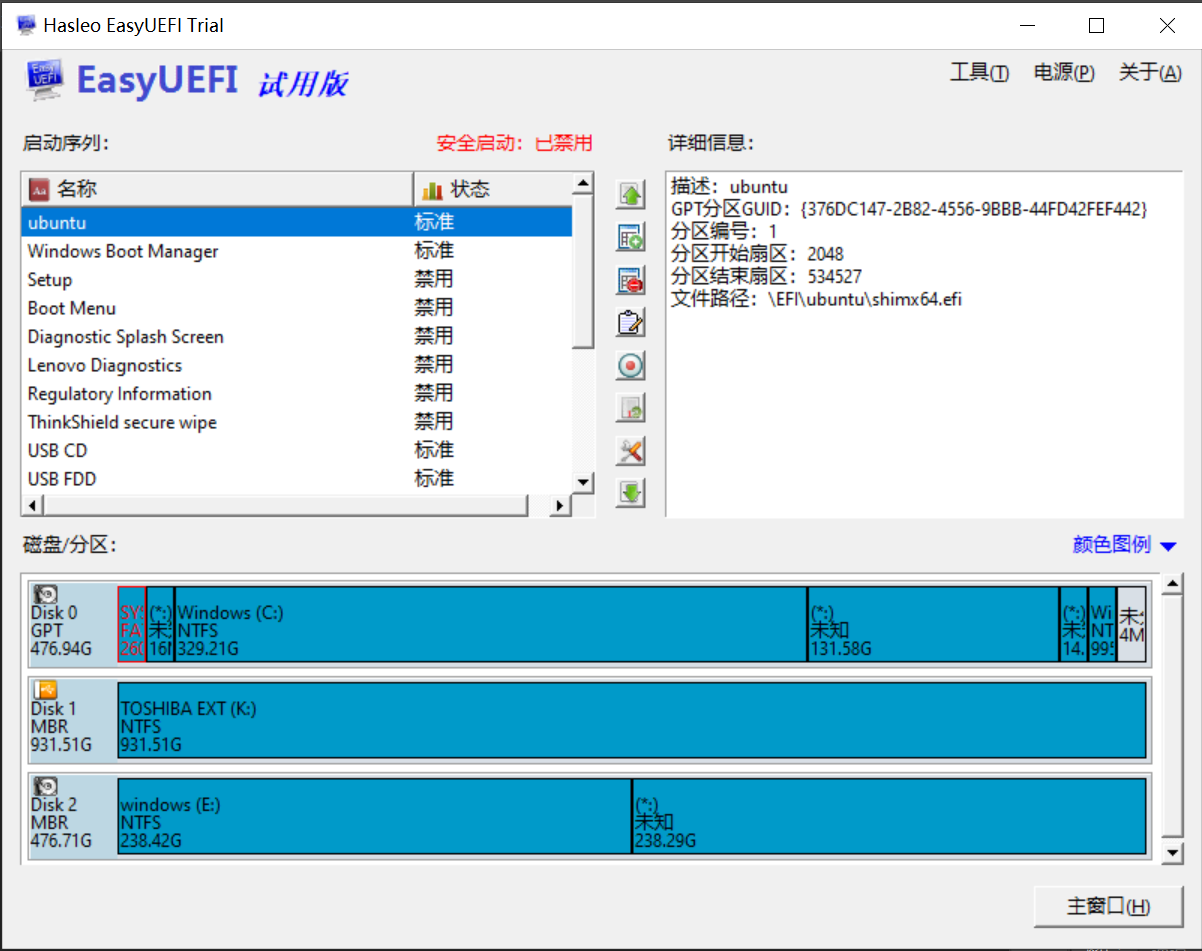
\includegraphics[width=0.75\textwidth]{png/easyuefi}
			 		\caption{检查efi启动项。}
			 		\label{fig:uefi}
				\end{figure}
                        \item [III-b.] 其他问题。双系统无法启动的原因可能很多,无法在此一一列举。主要问题都和efi内容有关。比如请仔细检查II-a项中的准备工作是否已经做了。
                \end{itemize}
\end{itemize}


\subsection{Ubuntu 上的软件安装}

如果你已经成功的安装了 Ubuntu 系统,
那么接下来你应该做的是在这个系统里面安装一些你需要的软件来丰富它。
在 Ubuntu 中安装软件和 Windows 系统中双击 exe 文件安装软件的方式有很大的不同,
在 Ubuntu 中主要有以下两种安装的方式。

\textbf{命令行安装:} Ubuntu 上软件安装的最常见方式是直接在终端(Ctrl+Alt+T)输入相应安装命令。
常见的有
\begin{itemize}
	\item apt-get安装;
	\item dpkg安装;
	\item 编译安装。
\end{itemize}

apt-get 安装是最常见的安装方式,其基本的安装命令为
\begin{verbatim}
sudo apt-get install package  // package 为需要安装的软件。
\end{verbatim}

区别于 apt 安装方式,dpkg 只是用来安装本地软件包(deb包),但不解决模块的依赖关系。
而 apt 是从网络服务器下载并安装软件包的,它会解决依赖关系。
其基本的安装命令为
\begin{verbatim}
sudo dpkg -i package.deb。
\end{verbatim}
由于 dpkg 的安装方式不会解决依赖的问题,所以经常会出现安装过程中依赖未安装的情况,
可以通过
\begin{verbatim}
sudo apt install -f	
\end{verbatim}
来修复依赖。

对于一些需要自己下载源代码编译安装的情况,
首先解压进入文件夹,一般都会有 README 或 install 文件指导你安装的过程,
通常过程为
\begin{verbatim}
./configure
make
sudo make install。
\end{verbatim}

\textbf{软件包管理器安装:}软件包管理器是 Ubuntu 的包管理工具 apt 的图形化前端。
它结合了图形界面的简单操作和 apt-get 命令行工具的强大功能。
它能跟踪所有已安装的软件、自动化进行安装和删除应用程序、
以及确保所有软件都保持更新以获得最新的增强功能和错误修复。
我们所需要做的仅仅是决定我们想安装哪个应用程序,
然后使用软件包管理器来告诉 Ubuntu 去安装它们。
常见的有
\begin{itemize}
	\item Ubuntu 软件中心;
	\item 新立得软件包管理器。
\end{itemize}

Ubuntu 软件中心是最容易使用的,它能让你安装和卸载许多流行软件包。
你可以简单地搜索如 'emacs' 这种关键字来搜索您想安装的软件包,或浏览给出的分类,
选择应用程序,将进入应用程序介绍页面,此页面将给出应用程序截图和简要介绍,
点击下方的“安装”按钮,获得授权后即开始安装软件。
\begin{figure}[htbp]
	\centering
	\subfigure[Ubuntu 软件中心界面]{
		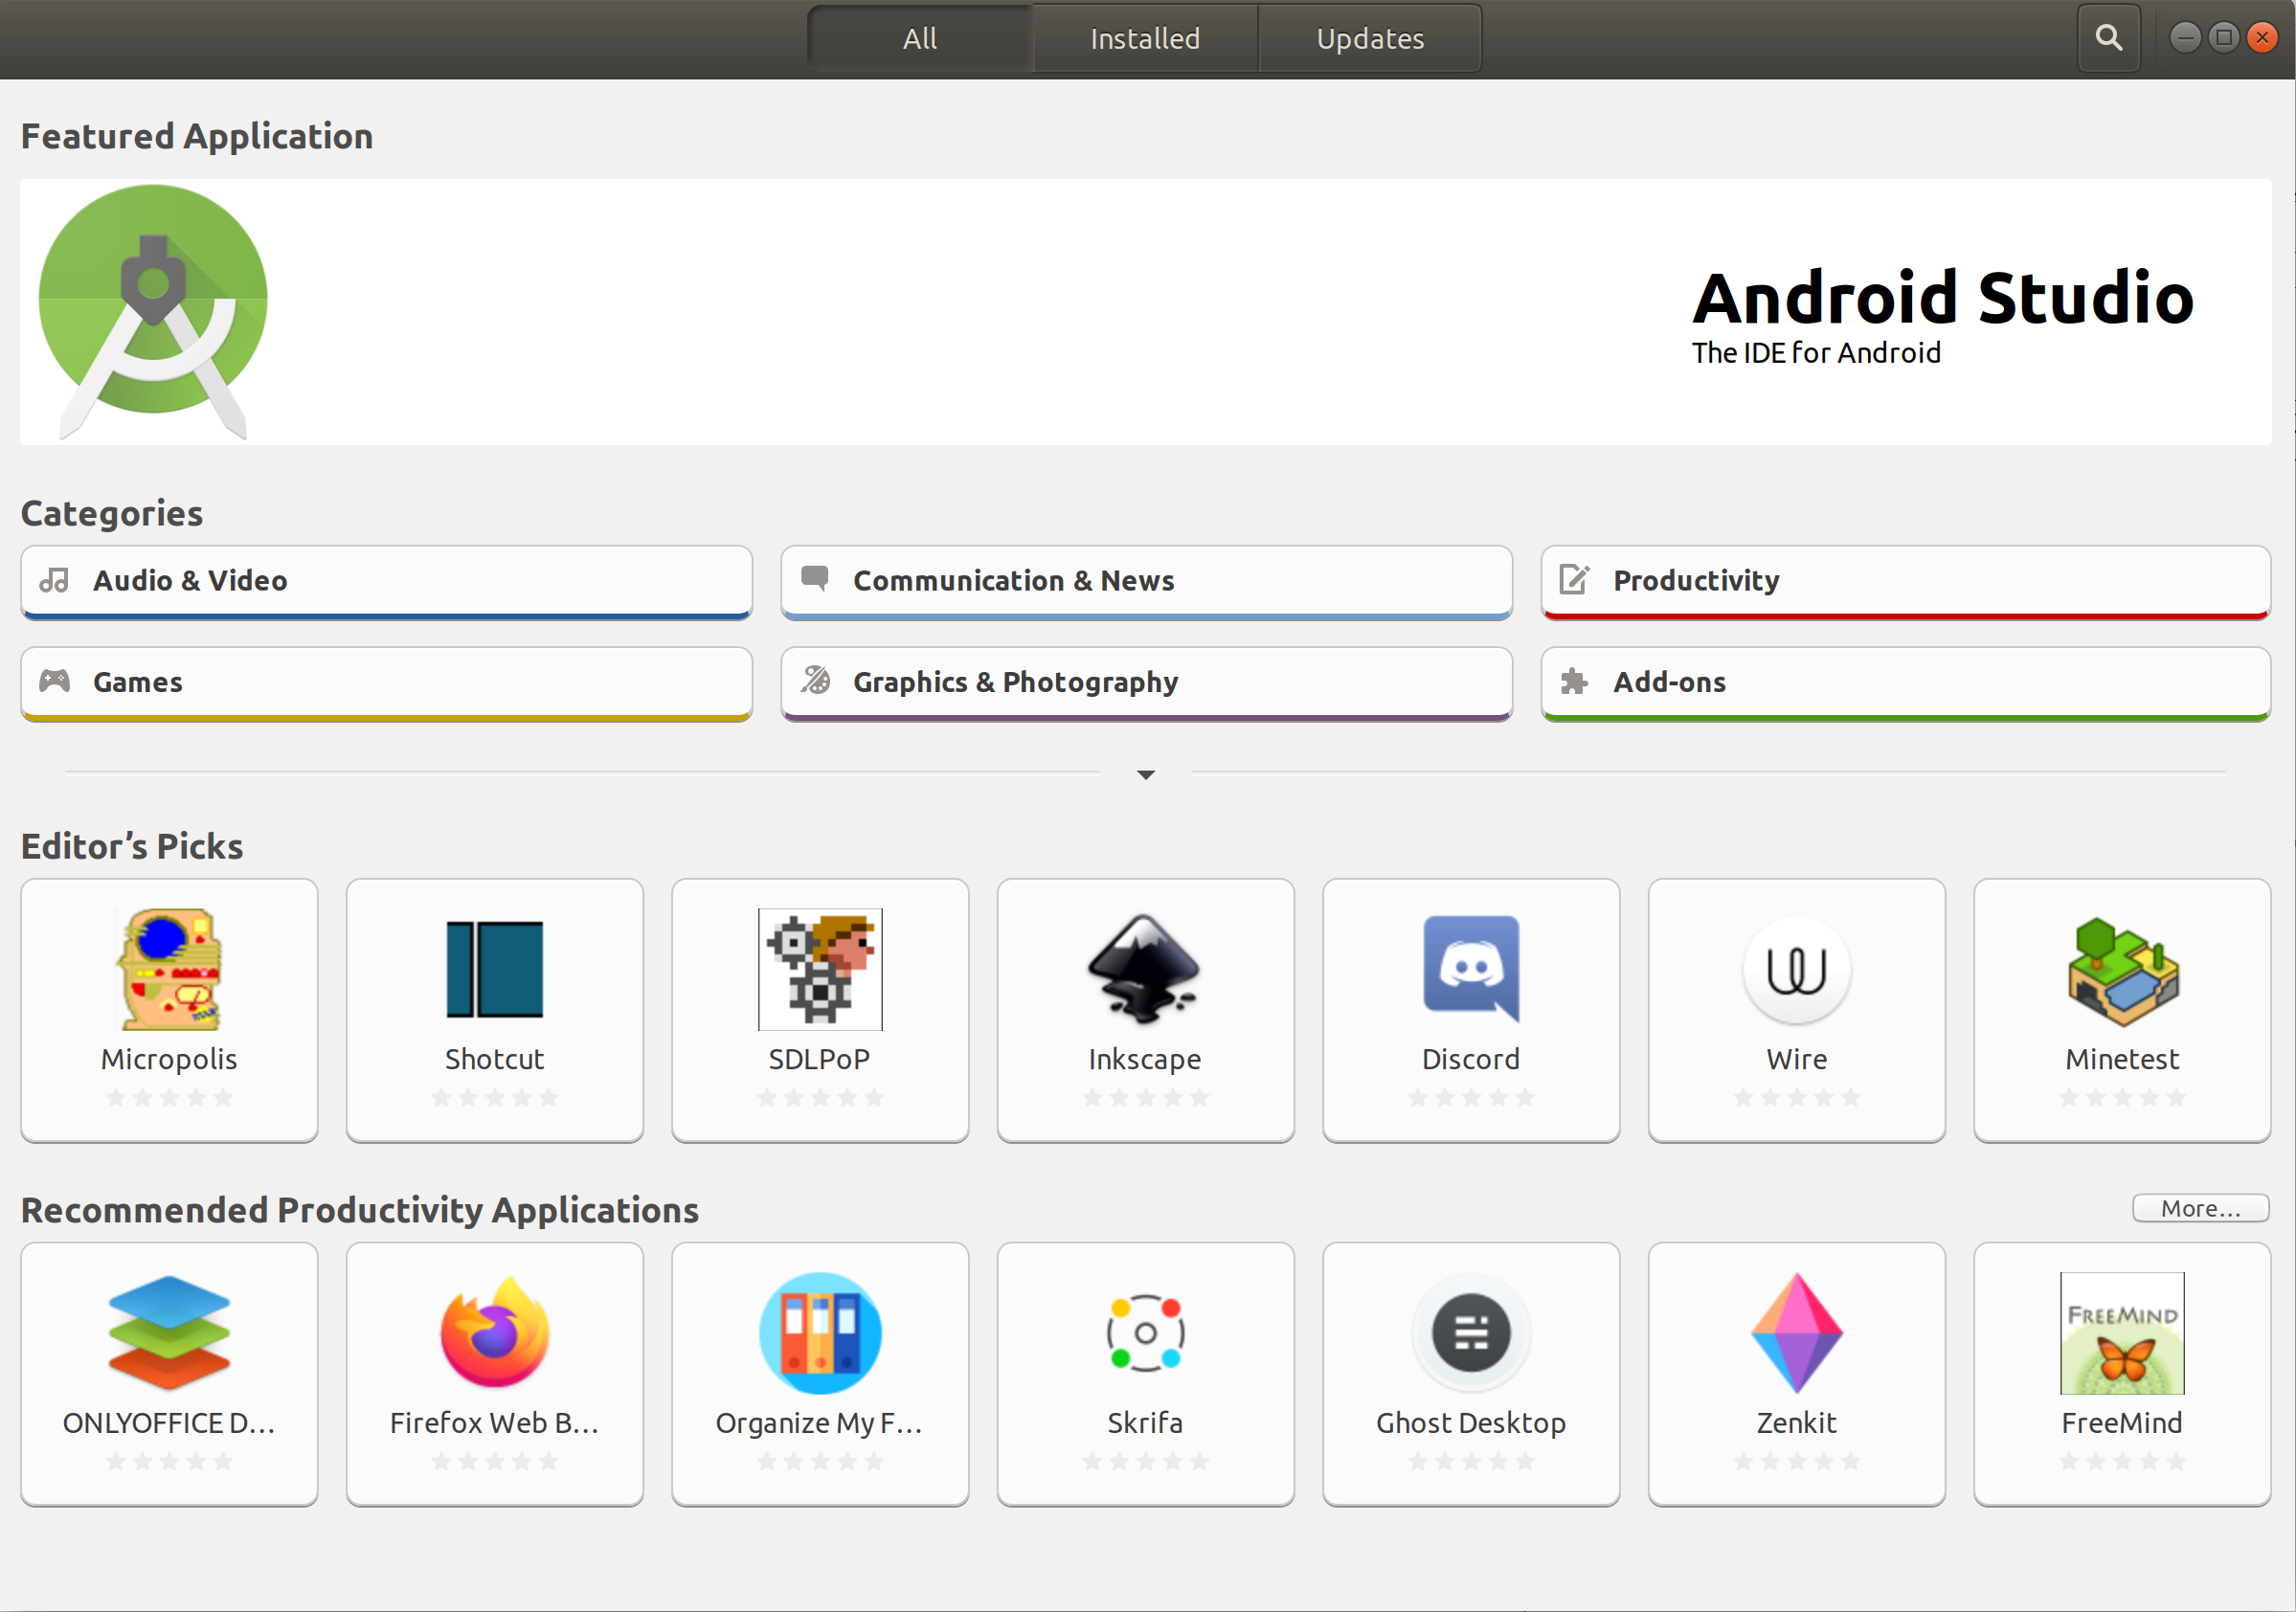
\includegraphics[width=0.45\linewidth]{png/ubuntuSoftware}
	}
	\hfill
	\subfigure[使用 Ubuntu 软件中心安装软件]{
		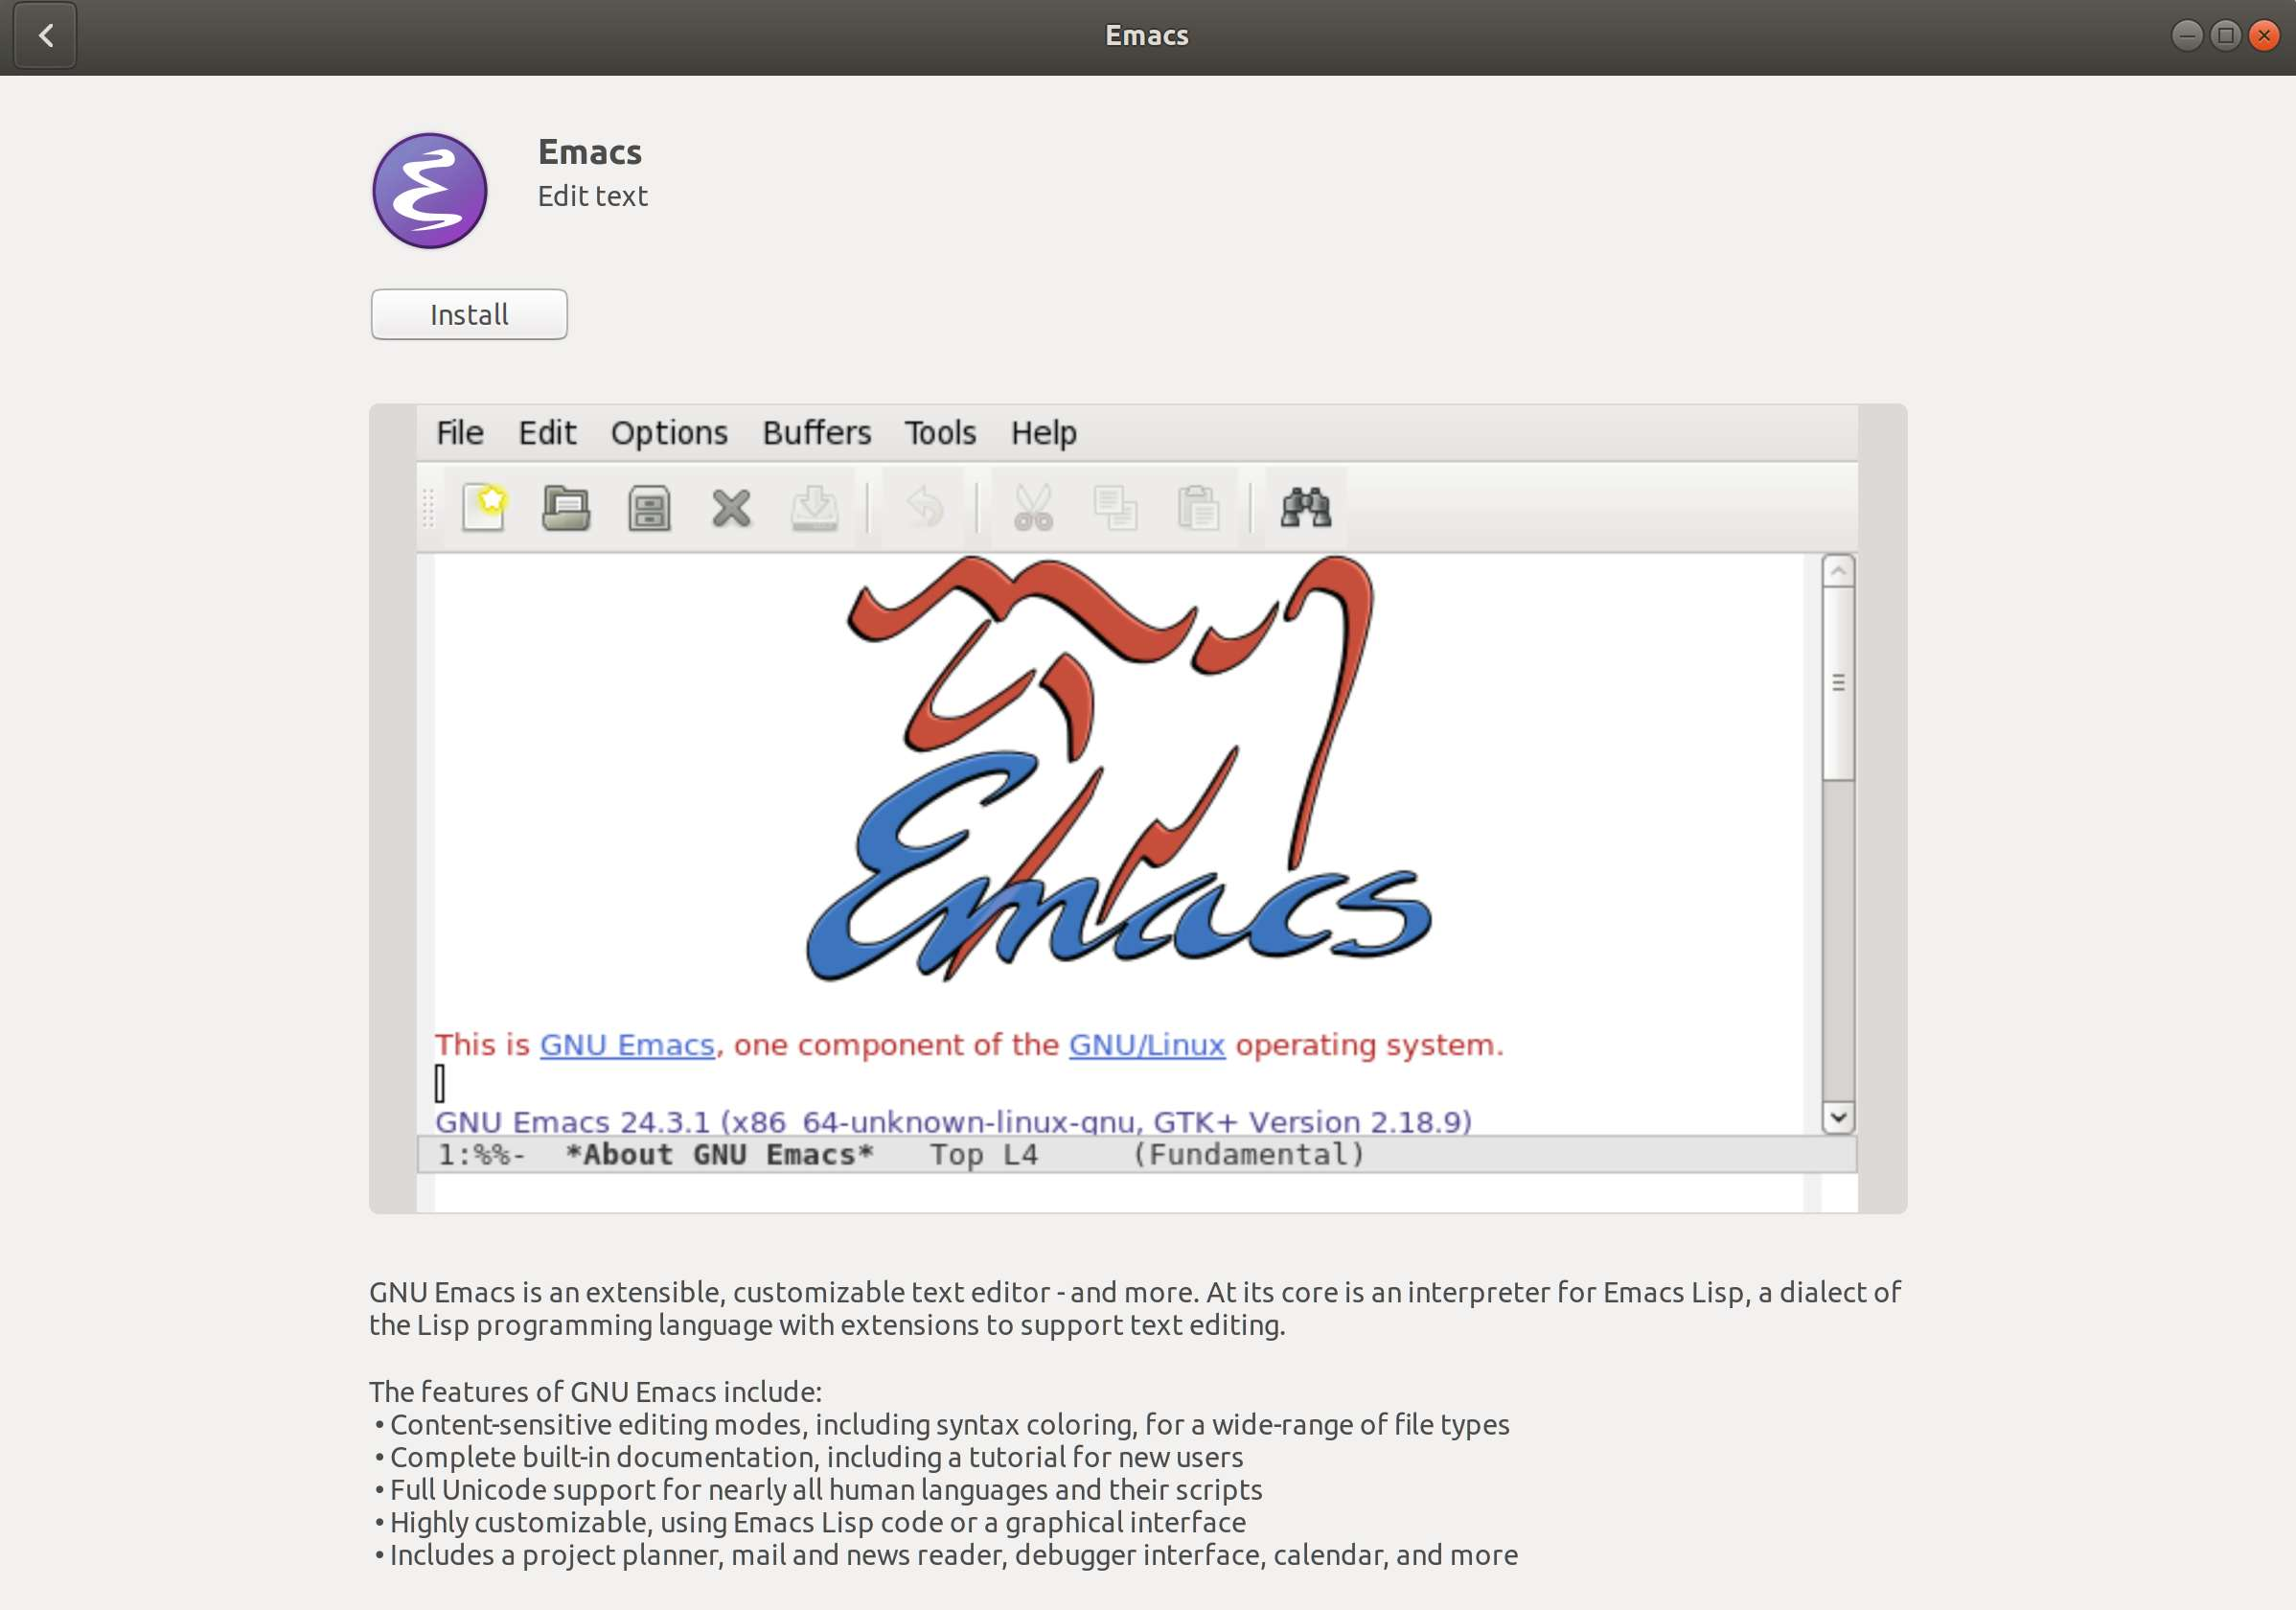
\includegraphics[width=0.45\linewidth]{png/emacsInstall}
	}
	\label{fig:Software}
\end{figure}

使用 Ubuntu 软件中心无法让您安装和删除某些更高级的软件包,
比如 Apache 网络服务、PHP 编程语言或 Scribus。这时,就得用新立得软件包管理器。
如果你的 Ubuntu 系统没有默认安装新立得软件包管理器(Synaptic Package Manager),
使用前需要安装它,基本命令为
\begin{verbatim}
sudo apt-get install synaptic。
\end{verbatim}

在新立得软件包管理器对话框中,你可以选择你需要的软件包。
左侧面板列出的是分类,右侧面板列出的是软件包。
点击搜索,将弹出查找对话框。在搜索字段中输入软件包的名称并点击搜索。
然后选择查找到的软件包,标记以便安装复选框来安装软件包。
如果你选择删除或安装的软件包依赖于其他软件包,你将得到依赖关系的通知。
点击标记以继续作出更改。
最后确认你想要进行标记的更改,点击应用即可自动安装。
\begin{figure}[htbp]
	\centering
	\subfigure[新立得软件包管理器界面]{
		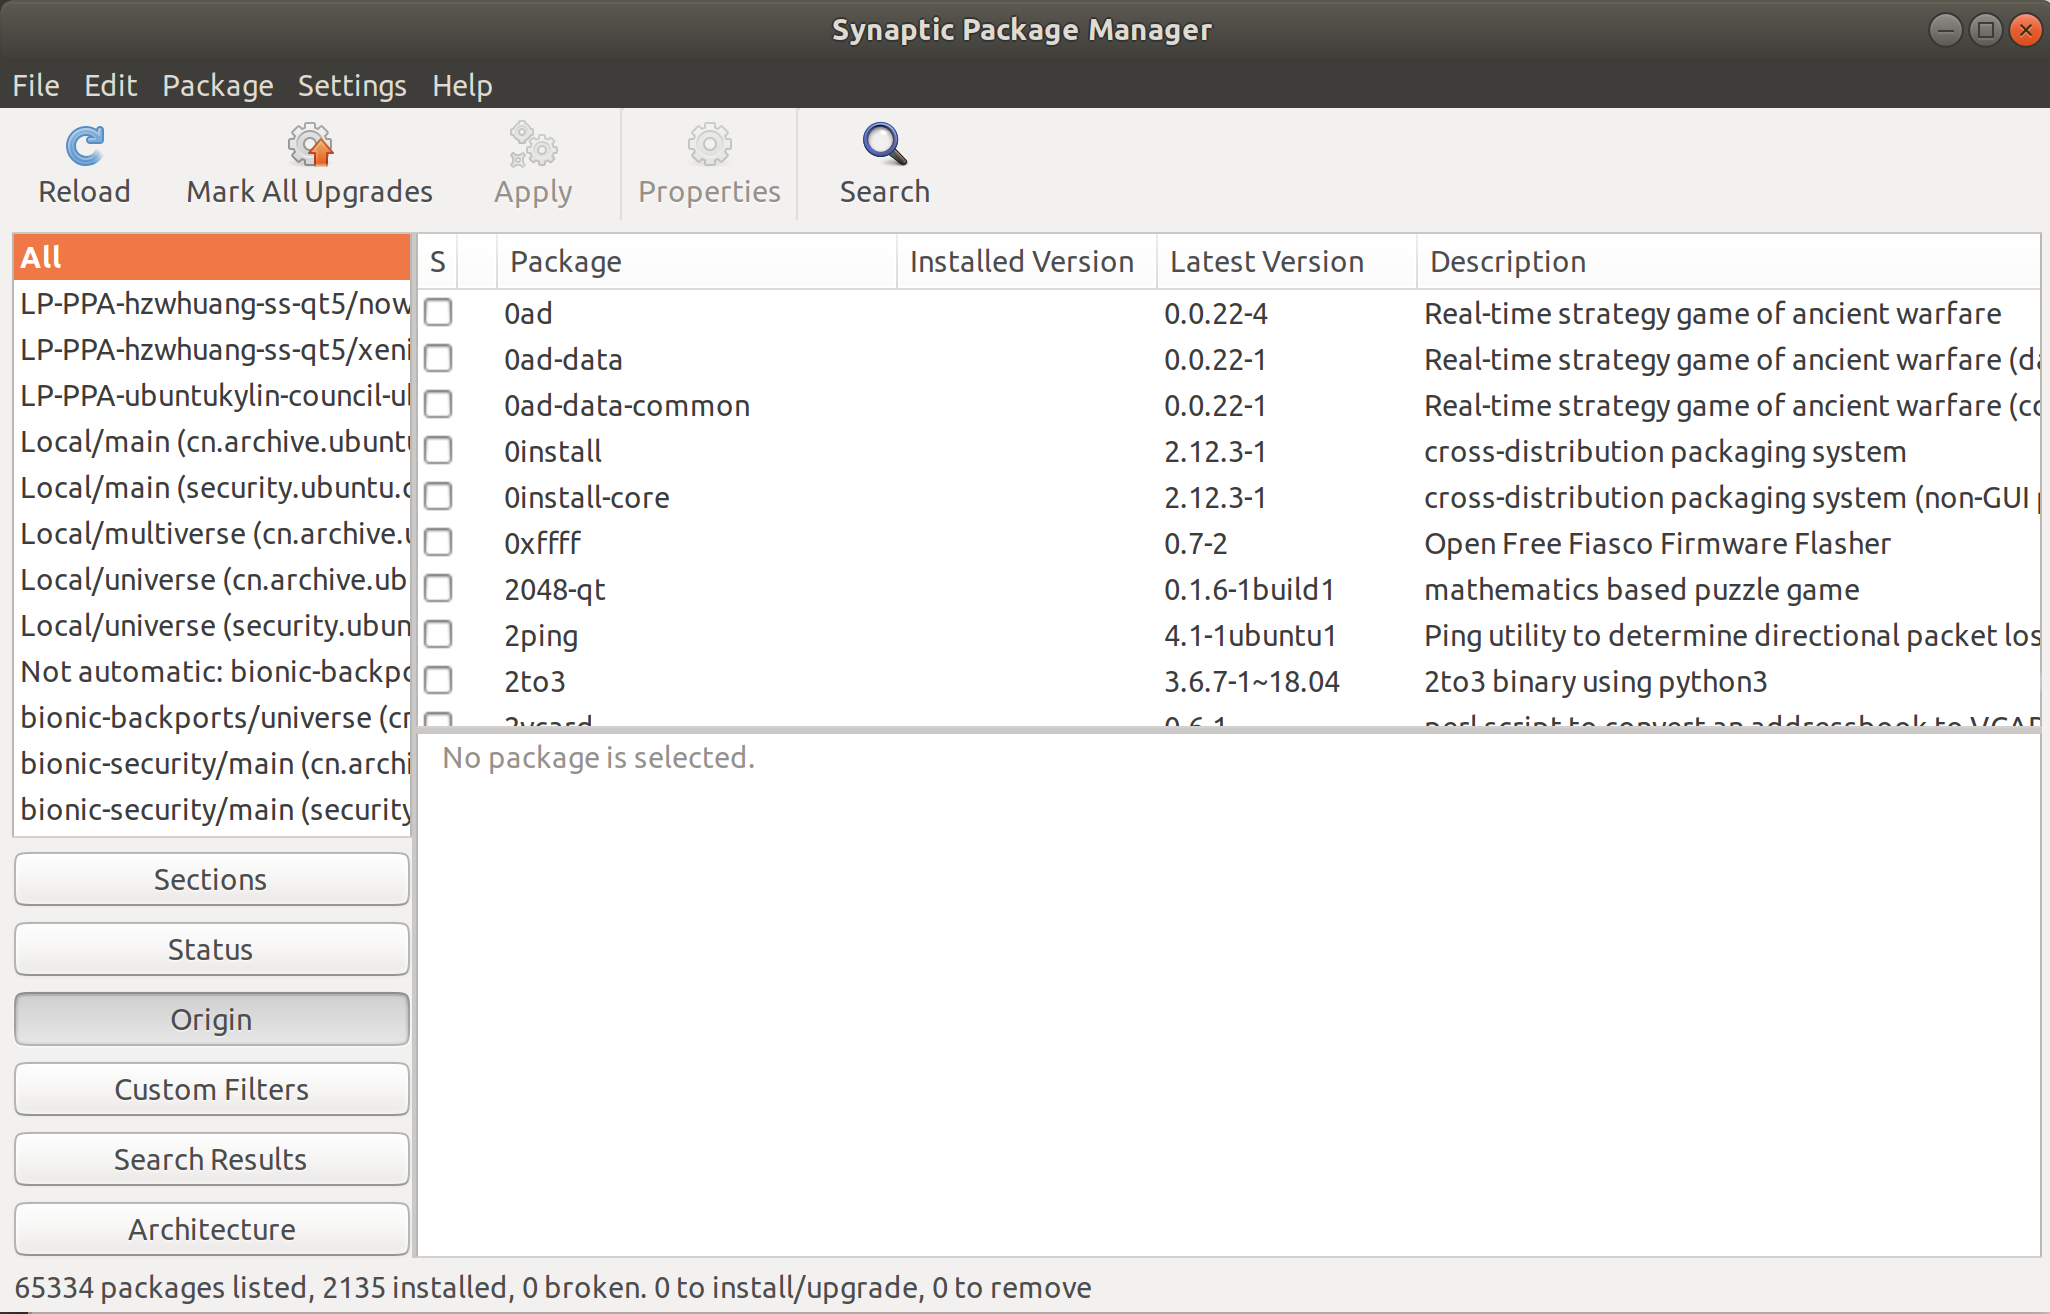
\includegraphics[width=0.45\linewidth]{png/synaptic}
	}
	\hfill
	\subfigure[使用新立得软件包管理器安装软件]{
		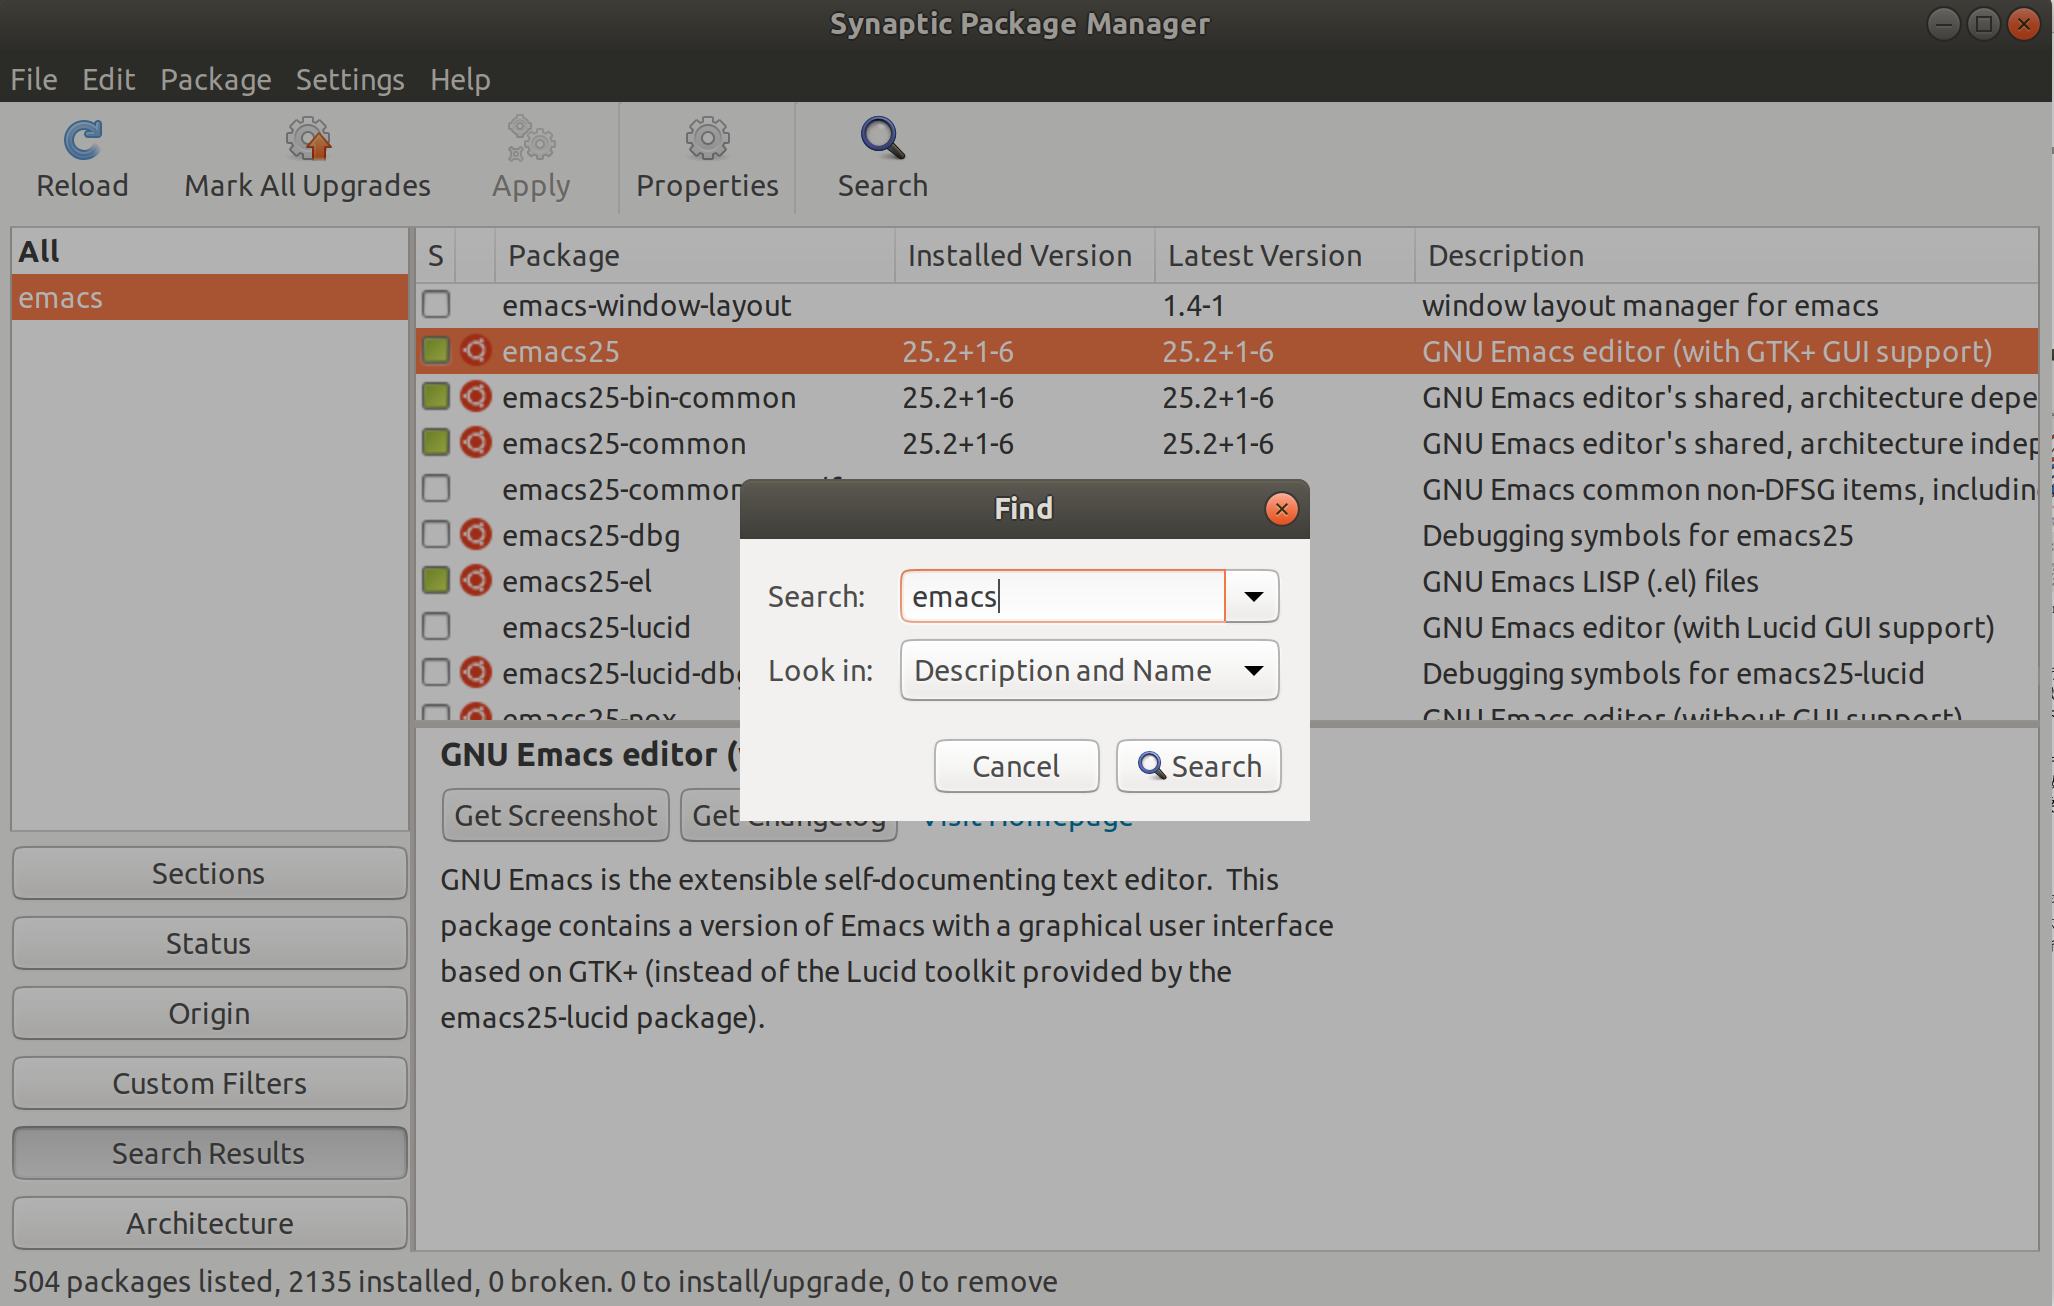
\includegraphics[width=0.45\linewidth]{png/synapticInstall}
	}
	\label{fig:Synaptic}
\end{figure}

\begin{remark}
	不得不提出的是,当你在体验一个新的操作系统的时候,难免会遇到各种各样的问题,
	要学会在使用的过程中进步,牢记常用的命令,养成不会就查的习惯!
\end{remark}






%%% Local Variables:
%%% mode: latex
%%% TeX-master: "../Guide"
%%% End:


\section{强大的文本编辑器---Emacs}
\label{sec:emacs}

Emacs 是一个强大的集成开发环境,
我们可利用它写代码、编译、调试、写文档,
我们甚至可以利用它上网,浏览网页,看视频,收发邮件等,
使用它可以极大地提高我们的工作效率。
学习 Emacs 的关键在于牢记各种快捷键,
减少在键盘和鼠标间的切换。
对于初学者建议按如下步骤学习 Emacs:
\begin{itemize}
	\item 阅读 Emacs Tutorial(进入 Emacs 后使用快捷键 Ctrl-h t)。
		其主要介绍基本的文本查看,编辑和查找操作,
		目的是让初学者对 Emacs 有一个大体的认识。
	\item 如果你想更加深入的了解Emacs,可以阅读书籍 
		Learning GNU Emacs\cite{cameron1996learning}, 
		这里推荐阅读 Chapter 5,8,9。
	\item 此时的你已能解决大多数问题,若还想继续学习 Emacs 的高级功能,
		可以学习 Emacs Lisp 语言,
		参考书籍 An Introduction to Programming in Emacs Lisp
		\cite{chassell2004introduction}。
\end{itemize}
在这里我们不过多介绍 Emacs 中的快捷键,
因为你可以在阅读上面书籍的过程中频繁遇到。
Emacs是绝对值得投入时间和经历的,因为你的回报会远远高出投入。



\subsection{Emacs + AUCTeX}

Emacs + AUCTeX 是一个能极大限度提高 \LaTeX 编辑效率的编辑器。
这是因为其具有强大的快捷键系统,方便的自动补全,
完善的引用系统以及快捷的自定义模板与环境等等。
当然效率的提高程度取决于你对它们的熟悉程度,不要因为刚入手时的困境而放弃。
这里我们简单的介绍一下其使用方法


\begin{itemize}	
	\item \textbf{安装:}可以在终端输入以下命令
	\begin{verbatim}
	sudo apt-get install emacs texlive-full auctex latex-cjk-*
	\end{verbatim}
    当然也可使用 Synaptic Package Manager 进行上述软件的安装。

	\item \textbf{核心操作:}
	\begin{itemize}
  		\item 打开一个文件(C-x C-f + 文件名),该命令后总是跟随这目录/文件名的,
  			如果要打开的文件不存在,就创建新文件;
  		\item 保存文件(C-x C-s),退出Emacs(C-x C-c);
  		\item 编译文档(C-c C-c),预览(C-c C-v),编译文档并查看(C-c C-a)。 
	\end{itemize}

	\item \textbf{基本操作:}
	\begin{itemize}
		\item 插入环境:通过 C-c C-e + 环境类型 命令添加环境
			\begin{verbatim}
			\begin{环境类型}
			\end{环境类型}
			\end{verbatim}
			可以使用 TAB 键查看环境类型列表或者自动补全;
		\item 插入宏:通过 C-c + Enter 命令插入宏,
			接着输入命令名称(usepackage,doucument 等等),
			最后选择输入命令的参数(没有可直接回车)。
			如果需要,你也可以添加相应的标签(可选),
			同样可以使用 TAB 键查看宏类型列表或者自动补全; 
		\item 快速更改字体(这系列命令一致以 C-c C-f 为前缀),如
			\begin{verbatim}
			C-c C-f C-e  // 插入强调字体 \emph{};
			\end{verbatim}
		\item 插入各级标题:通过 C-c C-s 命令插入标题,
			接着输入章节层级(section,subsection 等等),
	    	最后输入标题内容即可;
		\item 进入数学环境:通过 C-c $\sim$ 命令进入数学环境,
			里面快捷键很多,可以在菜单栏查看;
		\item 选择,注释,编译片段文件:
			\begin{verbatim}
			C-c C-r  编译区域
			C-c ;    注释/取消注释区域
			\end{verbatim}
		\item Emacs 内预览(在 Preview 菜单栏内查看);
		\item 多文件管理。
			编写较大的文档时,
			通常会使用 include 或 input 命令将主要章节分离成独立的文件。
			这时就需要在编写子文件的时候,键入编译和预览命令时,
			AUCTeX 能主动定位主文档并执行命令。
			为了做成这件事,需要首先在 .emacs 中添加命令
			\begin{verbatim}
			;; Query for master file.
			(setq-default Tex-master nil)
			\end{verbatim}
			之后,在每次创建新文件的时候我们都需要指定该文件的主文件,
			其基本命令为
			\begin{verbatim}
			C-c _ 
			\end{verbatim}
			然后输入主文件路径信息即可(不显示指明路径即默认该文件为主文件)。
			在编辑子文件时,输入
			\begin{verbatim}
			C-c ^
			\end{verbatim}
			即可返回到主文件。
			在子文件输入编译或者预览命令即可实现全局编译与预览。
	\end{itemize}
\end{itemize}

值得注意的是,使用 AUCTeX 前你不得不学会一些 \LaTeX 的基本句法。
不过作为一个刚接触 \LaTeX 或者接触 \LaTeX 不久的初学者,
设计一个精美的文档是相对困难的,
这时可以适当参考一些优秀的模板(如,\url{http://www.latextemplates.com})。
利用这些模板,我们可以轻松的表达我们想写的内容而不是注重文档设计的形式。
但无论什么时候,都要记住一个原则,即\textbf{保持源码的简洁性}。
大至整个文档的设计,小到每个语法,
其目的是为了方便阅读或者修改。

对于一个科研工作者来说,仅仅会用 \LaTeX 写文档是远远不够的。
在学习的生涯中,你可能会有无数次的报告,展示,答辩等等。
相比于传统的 PPT 展示,
利用 beamer 制作学术讲稿更加方便,美观。
因为其兼容 \LaTeX 命令,对于现有文章中的定义、定理、公式、算法、代码、图表等复杂内容,
只需要简单粘贴到 beamer 里面直接使用即可。
并且其输出为 PDF,具有很强的可读性,跨平台显示也无差异。
下面是一个简单的例子(其效果图见 \ref{fig:beamer}):
\begin{verbatim}
%!TEX program = xelatex

\documentclass{beamer}
\usepackage{xeCJK}

% 使用的主题,Beamer 因为有各种主题才使得有生气
\usetheme{Madrid}

\title[简短的标题]{这是一个简单的 \LaTeX 展示}
\author[作者]{xxx}
\institute[作者机构]{作者机构/信息}
\date[\today]{\today}

\begin{document}

% 标题页帧
\frame{\titlepage}
% 普通帧
\begin{frame}\frametitle{标题}
  这里是需要表达的内容!通常包括基本的文本,表格,图片等等!
\end{frame}

\end{document}
\end{verbatim}

\begin{figure}[htbp]
	\centering
	\subfigure[标题页帧]{
		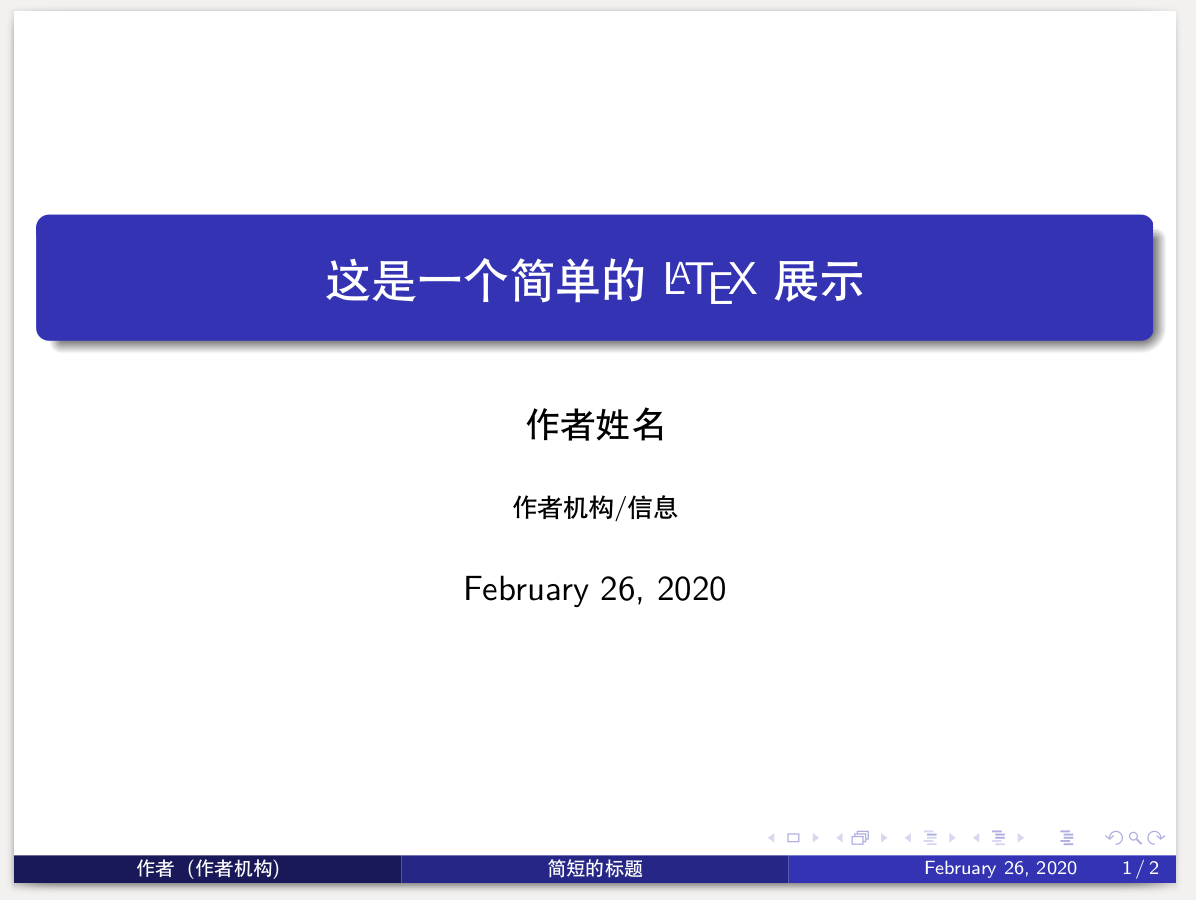
\includegraphics[width=0.48\linewidth]{png/beamer1}
	}
	\hfill
	\subfigure[普通帧]{
		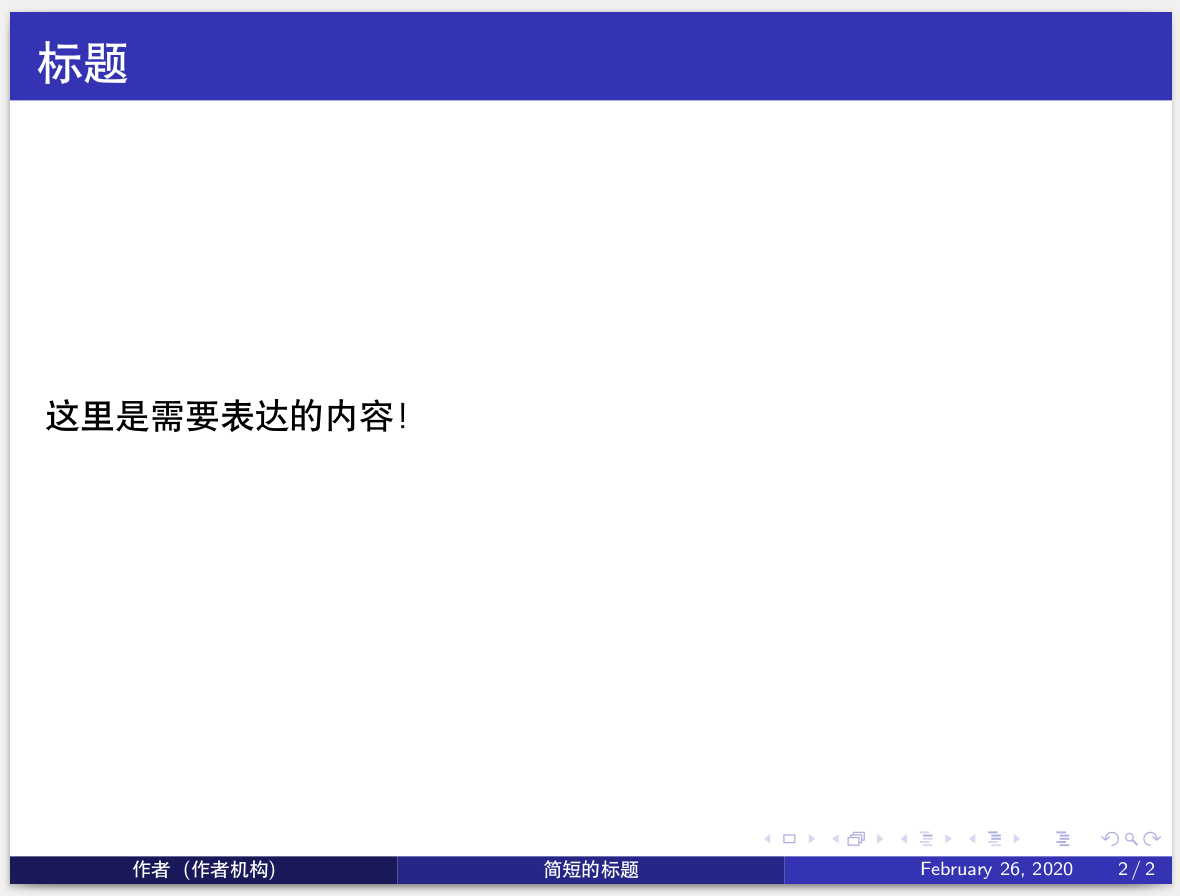
\includegraphics[width=0.48\linewidth]{png/beamer2}
	}
        \caption{标题和普通帧。}
	\label{fig:beamer}
\end{figure}

这里我们看到的每一页 PDF 即是所谓幻灯片的帧(frame),
Beamer 的帧分为两类,即
\begin{itemize}
	\item 标题页帧,语法为:
	\begin{verbatim}
	\frame{\titlepage}
	\end{verbatim}
	在这上面,一般会有标题、作者、时间、机构,LOGO等信息。
	\item 普通帧,主要为需要展示的内容,基本语法为:
	\begin{verbatim}
	\begin{frame}\frametitle{标题}
  	这里是需要表达的内容!
	\end{frame}
	\end{verbatim}
\end{itemize}

最后我们简要介绍一下 \LaTeX 中的作图工具---PSTricks。
它是一个基于 PS 的宏包,有了它我们就可以直接在 \LaTeX 文档中绘制非常复杂的图形。
但其命令繁琐,不太直观,所以不易熟练掌握。
初期,我们需要知道其基本语法,并学会绘制简单的图形。

\begin{itemize}
	
	\item 基本语法(因为 \LaTeX 绘图指令功能很弱,对较复杂的图形无能为力,
	一般都是用绘图软件事先将图形绘制好,再用图形输入命令插入 \LaTeX 源文件中,
	每一个图形的语法一般如下):
	\begin{verbatim}
	\documentclass[10pt]{article}

	\usepackage{amsmath}
	\usepackage{pstricks,pst-eps}
	\pagestyle{empty}

	\begin{document}
  	  \begin{TeXtoEPS}
    	\begin{pspicture}(5.5,5.5)

      	% Triangle in red:
      	\pspolygon[linecolor=red](1,1)(5,1)(1,4)
      	% Bezier curve in green:
      	\pscurve[linecolor=green,linewidth=2pt,%
      	showpoints=true](5,5)(3,2)(4,4)(2,3)
     	% Circle in blue with radius 1:
      	\pscircle[linecolor=blue,linestyle=dashed](3,2.5){1}

    	\end{pspicture}
  	  \end{TeXtoEPS}
	\end{document}
	\end{verbatim}
	其中紧跟在 pspicture 环境后面的 $(x_0,y_0), (x_1,y_1)$ 参数表示所绘制图形的大小,
	这个图形左下角的坐标在 $(x_0,y_0)$(不显示指明默认为原点),
	右上角的坐标在 $(x_1,y_1)$,生成的图形不能越过这个长方形的范围。
	每一个基本命令包括图形对象和图形参数。
	简单的如点、 线段,复杂的如各种曲线或自定义的图形都被称为图形对象。
	一个图形对象对应着一条命令, 一般的形式是
	\begin{verbatim}
	命令 [选项] ... 
	\end{verbatim}	
	其中选项可以是一个,也可以有多个,多个选项之间用逗号分隔。
	选项中一般设置绘制对象时的线条、颜色属性,这些属性又被称为图形参数。
	详细命令可以参考书籍
	PSTricks : PostScript macros for Generic TeX \cite{van1993pstricks}。
	\item Makefile 文件(负责由源代码生成 eps 格式图片):
	\begin{verbatim}
	allEps : test.eps
	clean :
   		rm *.aux *.log *.cache
	%.eps : %.dvi
   		dvips $< -E -o $@
	%.dvi : %.tex
   		latex $<
	\end{verbatim}
\end{itemize}

最后只需要在终端输入 make,
即可以得到我们想要绘制的图形(见 \ref{fig:pstricks})。

\begin{figure}[htbp]
	\centering
	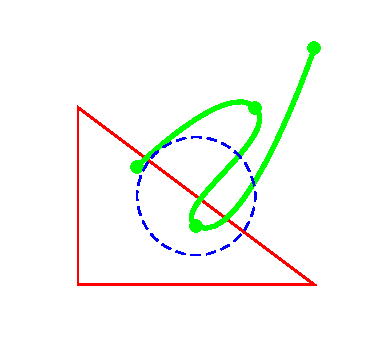
\includegraphics[width=0.4\textwidth]{eps/pstricks}
	\caption{使用 PSTricks 绘制的图片。}
	\label{fig:pstricks}
\end{figure}




\section{一次编写,终身受益---Makefile}
\label{sec:make}

什么是 makefile?
或许很多 Winodws 的程序员都不知道这个东西,
因为那些 Windows 的 IDE 都为你做了这个工作,
但作为一个好的专业的程序员,makefile 还是要懂。
特别在 Linux 下的软件编译,你就不能不自己写 makefile 了,
会不会写 makefile,从一个侧面说明了一个人是否具备完成大型工程的能力。
因为,makefile 关系到了整个工程的编译规则。
一个工程中的源文件不计数,其按类型、功能、模块分别放在若干个目录中,
makefile 定义了一系列的规则来指定,
哪些文件需要先编译,哪些文件需要后编译,哪些文件需要重新编译,
甚至于进行更复杂的功能操作,
因为 makefile 就像一个 Shell 脚本一样,其中也可以执行操作系统的命令。
makefile 带来的好处就是——自动化编译,
一旦写好,只需要一个 make 命令,
整个工程完全自动编译,极大的提高了软件开发的效率。


\subsection{程序的编译和链接}

在进入 makefile 之前,
我们不得不先说一下程序编译的一些规范和方法,
一般来说,对于C、C++文件来说,
首先要把源文件(.c/.cpp文件)编译成中间代码文件,
在 Windows 下也就是 .obj 文件,
Ubuntu 下是 .o 文件,即 Object File,这个动作叫做编译。
然后再把大量的 Object File 合成执行文件,这个动作叫作链接。   

编译时,编译器需要检查的是语法,函数与变量的声明是否正确。
对于后者,通常是你需要告诉编译器头文件的所在位置
(头文件中应该只是声明,而定义应该放在C/C++文件中),
只要所有的语法正确,编译器就可以编译出中间目标文件。
一般来说,每个源文件都应该对应于一个中间目标文件。 
链接时,主要是链接函数和全局变量,
所以,我们可以使用这些中间目标文件来链接我们的应用程序。
链接器并不管函数所在的源文件,只管函数的中间目标文件。

由源文件生成可执行程序的基本命令为
\begin{verbatim}
g++ hello.cpp hello1.cpp hello2.cpp -o hello
\end{verbatim}
这里 g++ 是将 gcc 默认语言设为 C++ 的一个特殊的版本
(编译 .c 文件时为 gcc),
链接时它自动使用 C++ 标准库而不用 C 标准库。
-o 指定生成的可执行文件的名称。
然后在命令行中输入程序名可使之运行:
\begin{verbatim}
./hello。
\end{verbatim}

可以使用选项 -c 用来告诉编译器编译源代码但不要执行链接,
输出结果为 .o 文件。
文件默认名与源码文件名相同,只是将其后缀变为 .o。
例如,下面的命令将编译源码文件 hello.cpp 并生成对象文件 hello.o
\begin{verbatim}
g++ -c hellospeak.cpp。
\end{verbatim}

\subsection{Makefile的核心规则}

在正式写一个完整的makefile之前,
我们先来粗略地看一看makefile的规则,
即makefile三要素:
\begin{verbatim}
target : prerequisites
         command
\end{verbatim}

其中 target 可以是一个 object file(目标文件),
也可以是一个执行文件,还可以是一个标签。
\\prerequisites 就是,要生成 target 目标所需要的文件。
command 也就是 make 需要执行的命令。
需要注意的是这里的 command 前是一个 tab 键(不能使用空格)。
这是一个文件的依赖关系,
也就是说,target 这一个或多个的目标文件依赖于 prerequisites 中的文件,
其生成规则定义在 command 中。
说白一点就是说,rerequisites 中如果有一个以上的文件比 target 文件要新的话,
command 所定义的命令就会被执行。
这就是 makefile 的规则,也就是 makefile 中最核心的内容。

那么 makefile 是如何工作的呢?
在默认的方式下,也就是我们只输入 make 命令。
那么,
\begin{itemize}
	\item make 会在当前目录下找名字叫 Makefile 或 makefile 的文件
		(文件命名非常严格,只建议这两种命名方式)。
	\item 如果找到,它会找文件中的第一个目标文件 target),
		并把这个文件作为最终的目标文件。
	\item 如果目标文件不存在(尚未生成),
		或是目标文件所依赖的后面的文件的文件修改时间要比目标文件新,
		那么,他就会执行后面所定义的命令来生成目标文件。
	\item 如果目标所依赖的文件也不存在,
		那么 make 会在当前文件中找目标文件所依赖的文件的依赖性,
		按照上述规则执行。
	\item 最终 make 会一层又一层地去找文件的依赖关系,
		直到编译出第一个目标文件。
\end{itemize}



\subsection{一步步写好 makefile 文件}

我们先来看一个非常简单的例子,假设我们有 4 个文件,
它们分别是 main.cpp,add.cpp,\\ mul.cpp, sub.cpp;
其中 main.cpp 依赖于 add.cpp, mul.cpp, sub.cpp,
为了简单起见,假设 add.cpp,mul.cpp,sub.cpp 之间没有依赖关系。

一个最简单的 makefile 文件就是我们在命令行编译的时候输入的编译代码,
用 makefile 的规范书写就是
\begin{verbatim}
test : main.cpp add.cpp mul.cpp sub.cpp
   g++ -o test main.cpp add.cpp mul.cpp sub.cpp
\end{verbatim}

虽然这个 makefile 文件是可以正常运行的,但如果仅仅是这样,
似乎没有说起来那么神奇。
试想如果我们仅仅修改了 sub.cpp 文件,那么按照 makefile 的规则,
修改后的 sub.cpp 要比 test 新,程序又再次执行了
\begin{verbatim}
g++ -o test main.cpp add.cpp mul.cpp sub.cpp,
\end{verbatim}
这导致了其他不相关的文件 add.cpp,mul.cpp 又要重新编译,
这无疑浪费了很多资源。
基于此,我们可以考虑将编译链接过程分解出来,
即显示的让编译器先生成中间目标文件(.o文件),
修改后的 makefile 文件如下
\begin{verbatim}
test : main.o add.o sub.o mul.o
   g++ -o test main.o add.o sub.o mul.o
main.o : main.cpp
   g++ -c main.cpp
add.o : add.cpp
   g++ -c add.cpp
sub.o : sub.cpp
   g++ -c sub.cpp
mul.o : mul.cpp
   g++ -c mul.cpp
\end{verbatim}

虽然这样的 makefile 基本符合我们的需求,
但是写起来未免有些麻烦,拓展性也不是太强。
比如对于每个源文件,我们都要重新写一次它的编译过程,
即使它们的语法一模一样。
为了解决这个问题,下面我们介绍一些写 makefile 文件常用的技巧
\begin{itemize}
	\item 利用"\# 注释内容"可以添加注释,以此来增加 makefile 的可读性;
	\item 使用变量:在 makefile 中,
		我们可以利用变量来代表某些多处使用而又可能发生变化的内容,
		这样可以节省重复修改的工作,还可以避免遗漏。
		使用规则为
		\begin{verbatim}
		变量名称 = 值列表
		\end{verbatim}
		需要使用的时候可以用 "\$(变量名称)" 来替换即可。
		例如在上述 makefile 中,我们可以使用 ObjFiles 来代替所有的中间目标文件
		\begin{verbatim}
		#(注释) 定义和使用变量ObjFiles
		ObjFiles = main.o add.o sub.o mul.o
		test : $(ObjFiles)
  			 g++ -o test $(ObjFiles)
		...
		\end{verbatim}
	\item 使用函数,在这里我们仅仅介绍两个常用的函数
    \begin{itemize}
    	\item wildcard :扩展通配符;
    		通常用法是使用"\$(wildcard *.cpp)"来获取工作目录下的所有的 .cpp 文件列表。
    	\item patsubst :替换通配符;
    		通常用法是使用"\$(patsubst\%.cpp,\%.o,\$(wildcard *.cpp))"
    		得到在当前目录下可生成的 .o 文件列表。
    		原理为先使用 wildcard 函数获取工作目录下的 .cpp 文件列表,
    		之后将列表中所有文件名的后缀 .cpp 替换为 .o。
    \end{itemize}
    使用函数后的 makefile 文件
	\begin{verbatim}
	# get all .cpp files
	SrcFiles = $(wildcard *.cpp)
	# get all .o files
	ObjFiles = $(patsubst %.cpp,%.o,$(wildcard *.cpp))
	test : $(ObjFiles)
   		g++ -o test $(ObjFiles)
	... 
	\end{verbatim}
	
	\item makefile 的模式匹配规则:
		目标名中需要包含有模式字符 \%(一个),
		包含有模式字符 \% 的目标被用来匹配一个文件名, 
		\% 可以匹配任何非空字符串。
		规则的依赖文件中同样可以使用 \%,
		依赖文件中模式字符 \% 的取值情况由目标中的 \% 来决定。
		最常用的用法是把所有的源文件生成中间目标文件。
		\begin{verbatim}
		%.o : %.cpp
   			g++ -c $< -o $@ 
		\end{verbatim}
		其中规则命令行中使用了自动化变量 \$ <和 \$@。
		自动化变量\$ < 代表规则的依赖,\$@ 代表规则的目标。
		此规则在执行时,命令行中的自动化变量将根据实际的目标和依赖文件取对应值。
		这样一个基本的拓展性强的 makefile 文件初步生成了
		\begin{verbatim}
		# get all .c files
		SrcFiles = $(wildcard *.cpp)
		# get all .o files
		ObjFiles = $(patsubst %.cpp,%.o,$(wildcard *.cpp))
		test : $(ObjFiles)
   			g++ -o test $(ObjFiles)
		%.o : %.cpp
   			g++ -c $< -o $@ 
		\end{verbatim}
	\item 每个 makefile 中都应该写一个清空目标文件(.o和执行文件)的规则,
		这不仅便于重新编译,也很利于保持文件的清洁。
		这是一个基本修养。
		一般的风格都是:
		\begin{verbatim}
		clean: 
   			rm + 需要清理的文件
		\end{verbatim}		
		更为稳健的做法是:
		\begin{verbatim}
		.PHONY : clean
		clean :
   			-@rm -f 需要清理的文件 
		\end{verbatim}	
		其中 .PHONY 意思表示 clean 是一个伪目标(防止产生冲突)。
		而在 rm 命令前面加了一个小减号的意思就是,
		也许某些文件出现问题,但不要管,继续做后面的事。
		@表示不在命令行显示这个命令,
		-f表示强制执行,不管有没有这些文件。
		值得注意的是,clean 的规则不要放在文件的开头,
		不然,这就会变成make的默认目标,相信谁也不愿意这样。
		不成文的规定是——clean 从来都是放在文件的最后。
		有时也可以添加 realclean 进行更深层次的清理。
	\item 添加伪目标 all:因为 makefile 默认第一个目标是"终极目标",
		所以我们约定的做法是使用一个称为"all"的伪目标来作为终极目标,
		它的依赖文件就是那些需要创建的程序。
		\begin{verbatim}
			all : 其他目标
		\end{verbatim}
	\item 添加 run 来运行程序。
	
\end{itemize}

我们展示一下最后的 makefile 文件
\begin{verbatim}
CPP = g++
OFLAG = -o
CFLAG = -c

.PHONY: clean all

all: test

# get all .cpp files
SrcFiles = $(wildcard *.cpp)
# get all .o files
ObjFiles = $(patsubst %.cpp,%.o,$(wildcard *.cpp))

test : $(ObjFiles)
   $(CPP) $(OFLAG) $@ $(ObjFiles)

%.o : %.cpp
   $(CPP) $(CFLAG) $< $(OFLAG) $@ 

run:
   ./test

clean:
   -@rm -f *.o
\end{verbatim}
这样我们只需要在终端输入 make,make run 或者 make clean 
就可以实现程序的编译,运行以及清理工作。






















%%% Local Variables:
%%% mode: latex
%%% TeX-master: "../Guide"
%%% End:


\section{软件调试的艺术---GDB}
\label{sec:gdb}

\subsection{传统的调试技巧}

在你还没有接触过 gdb 之前,程序遇见了问题你会怎么办?
传统的调试技巧只是向程序中添加跟踪代码以在程序执行时输出变量的值,
例如使用 printf() 或 cout 语句输出变量的值。
你可能会问:"这样操作够吗?为什么还要使用 GDB 这样的调试工具?"

首先,这种方法要求有效率的持续添加跟踪代码,重新编译程序,
运行程序并分析跟踪代码的输出,在修正错误之后删除跟踪代码,
并且针对发现的每个新的程序错误重复上述这些步骤。
这种工作过程非常耗时,并且容易令人疲劳。
最为重要的是,这些操作将你的注意力从实际任务转移开,
并且降低了集中精力查找程序错误所需的推理能力。
在这种情况下,Linux 为我们程序调试提供了一种神器,即 GDB 调试。
使用 GDB,我们可以随时查看变量的值,随时停住我们的程序,
而这些只需要一些简单的命令即可实现。

\subsection{gdb中的基本命令}
大多数 Linux 系统应该预先安装了 GDB。
如果没有预先安装该工具,则必须下载 GCC 编译器程序包,
其安装命令为
\begin{verbatim}
sudo apt-get install gcc gdb。
\end{verbatim}

启动 gdb 的命令是
\begin{verbatim}
gdb yourpram,
\end{verbatim}
这里 yourpram 是你的可执行程序文件(文件是经过编译之后形成的可执行文件),
在编译时,应该加上 -g 选项
(这里是为了增加调试信息,如创建符号表,关闭所有的优化机制等等),
比如
\begin{verbatim}
gcc -o test_gdb test_dgb.c -g。
\end{verbatim} 

下面我们列举一些在 GDB 中一些常规的基本操作,
\begin{itemize}
	\item 在 GDB 中启动程序:
	\begin{itemize}
		\item run/r (GDB允许在不产生歧义的情况下使用缩写) 启动,程序会自动运行到下一个断点;
		\item start 启动,程序会停留在 main 函数处,方便后续分步调试;
	\end{itemize}
	\item 执行下一条语句:
	\begin{itemize}
		\item next/n,如果该语句为函数调用,不会进入函数内部执行(即不会一步步地调试函数内部语句);
		\item step/s,如果该语句为函数调用,则进入函数执行其中的第一条语句;
	\end{itemize}
	\item 在 GDB 中设置启动参数:set args 参数1 参数2;也可以使用 run + 参数1 参数2;
	\item list/l,默认显示 10 行源代码(带有主函数的源文件),回车可继续显示 10 行;
		如果想要查看某个文件的源代码,使用 list + 文件名:行号;
	\item 在 GDB 中设置断点(程序运行的时候会停留在断点处):
	\begin{itemize}
		\item break/b + 行号,指定行数处设置断点(默认为主文件所在行数);
		\item break/b + 函数,指定函数处设置断点;
		\item break/b + 文件名:行号,指定某个文件的某行处设置断点;
		\item break/b + 行号 + if ...,设置条件断点;
	\end{itemize}
	\item 查看断点信息:info break/b;
		删除断点:del/d + 断点编号(删除断点前需要先查看断点编号信息);
	\item continue/c,继续执行程序直到下一个断点或者程序结束;
	\item 使用 print/p 打印变量的值,ptype 打印变量的类型;
	\item set varname = v,在程序运行的时候设置变量的值;
	\item 使用 display/disp + varname 用来跟踪某个变量,查看变量什么时候变化,
		程序每次停下来的时候都会显示它的值。同样可以使用 undisplay + 跟踪变量编号 放弃跟踪;
	\item 使用命令 quit 退出 GDB。
\end{itemize}

下面是一个调试段错误的详细示例。利用你学习的知识,找出其中的问题
\begin{verbatim}
//
// insertion sort, several errors
//
// usage:  insert_sort num1 num2 num3 ..., where the numi are the numbers to
// be sorted

int x[10],  // input array
    y[10],  // workspace array  
    num_inputs,  // length of input array
    num_y = 0;  // current number of elements in y

void get_args(int ac, char **av)
{  int i;

   num_inputs = ac - 1;
   for (i = 0; i < num_inputs; i++)
   x[i] = atoi(av[i+1]);
}

void scoot_over(int jj)
{  int k;

   for (k = num_y-1; k > jj; k++)
     y[k] = y[k-1];
}

void insert(int new_y)
{  int j;

   if (num_y = 0)  { // y empty so far, easy case
     y[0] = new_y;
     return;
   }
   // need to insert just before the first y 
   // element that new_y is less than
   for (j = 0; j < num_y; j++)  {
     if (new_y < y[j])  {
       // shift y[j], y[j+1],... rightward 
       // before inserting new_y
       scoot_over(j);
       y[j] = new_y;
       return;
     }
   }
}

void process_data()
{
   for (num_y = 0; num_y < num_inputs; num_y++)
     // insert new y in the proper place 
     // among y[0],...,y[num_y-1]
     insert(x[num_y]);
}

void print_results()
{  int i;

   for (i = 0; i < num_inputs; i++)
     printf("%d\n",y[i]);
}

int main(int argc, char ** argv)
{  get_args(argc,argv);
   process_data();
   print_results();
}
\end{verbatim}




\subsection{gdb追踪核心文件}

相信大部分人在编程的时候都会遇见过下面这种情形:
\begin{verbatim}
段错误 (核心已转储)。
\end{verbatim}

导致程序爆炸或者崩溃,这些程序错误通常与指针的误操作有关。
迄今最常见的导致程序崩溃原因是试图在未经允许的情况下访问一个内存单元。
在这里我们不去过多的解释内存访问错误是如何发生的,
而把重点放在如何处理这种问题上面。

核心文件(core文件)可以理解为程序崩溃时的"案发现场",
正确的使用core文件,调试器可以判断出程序错误所在的大概位置。
其使用步骤一般如下
\begin{itemize}
	\item 创建核心文件:
		\begin{verbatim}
		ulimit -c unlimited。
		\end{verbatim}
	\item 查看 core 文件:
		\begin{verbatim}
		gdb 可执行文件 core文件名。
		\end{verbatim}
\end{itemize}

\begin{remark}
	默认情况下,核心文件的命名约定比较简单,它们都称为 core。
	当有多个可执行程序时,它们产生的 core 文件名称一样,
	因此需要我们对核心文件的文件名进行设置。
	只需要在命令行输入
	\begin{verbatim}
	sudo su
	echo "core-%e-%t" > /proc/sys/kernel/core_pattern
	\end{verbatim}
	即可。
\end{remark}

下面是一个调试段错误的详细示例。利用你学习的知识,找出其中的问题
\begin{verbatim}
#include <stdio.h>
#include <stdlib.h>
#include <string.h>

typedef struct {
  char *str;
  int  len;
} CString;



CString *Init_CString(char *str)
{
  CString *p = malloc(sizeof(CString));
  p->len = strlen(str);
  strncpy(p->str, str, strlen(str) + 1);
  return p;
}


void Delete_CString(CString *p)
{
  free(p);
  free(p->str);
}


// Removes the last character of a CString and returns it.
//
char Chomp(CString *cstring)
{
  char lastchar = *( cstring->str + cstring->len);
  // Shorten the string by one
  *( cstring->str + cstring->len) = '0';
  cstring->len = strlen( cstring->str );

  return lastchar;
}


// Appends a char * to a CString
//
CString *Append_Chars_To_CString(CString *p, char *str)
{
  char *newstr = malloc(p->len + 1);
  p->len = p->len + strlen(str);

  // Create the new string to replace p->str
  snprintf(newstr, p->len, "%s%s", p->str, str);
  // Free old string and make CString point to the new string
  free(p->str);
  p->str = newstr;

  return p;
}


int main(void)
{
  CString *mystr;
  char c;

  mystr = Init_CString("Hello!");
  printf("Init:\n  str: `%s' len: %d\n", mystr->str, mystr->len);
  c = Chomp(mystr);
  printf("Chomp '%c':\n  str:`%s' len: %d\n", c, mystr->str, mystr->len);
  mystr = Append_Chars_To_CString(mystr, " world!");
  printf("Append:\n  str: `%s' len: %d\n", mystr->str, mystr->len);

  Delete_CString(mystr);

  return 0;
}
\end{verbatim}

%%% Local Variables:
%%% mode: latex
%%% TeX-master: "../Guide"
%%% End:




\chapter{方法篇}

\section{是什么? 为什么? 怎么做(用)?}
\label{sec:WhatWhyHow}

好的学习方法,一定是那些在你找到它之后简单易上手,
能够让你提高效率,化为自己独特技能的。
那么什么样的学习方法才能实现高效学习呢?
衡量一种方法是否高效的唯一标准就是看你完成目标时所花费的时间长短。
相同的一件事情,花费的时间越少,学习效率就越高。
在这里,我们提供一种基本的学习或者方法,那就是:
对待一个问题,学会找到是什么,为什么,怎么做(用)这三个基本点,建立思维树。
经验证明,这种方法是相对高效的。

\begin{itemize}
\item "是什么"是面对问题的一个最基本的层次,
  它就是数学中一个严谨的定义,不需要华丽的辞藻来修饰。
\item "为什么"更多的是一种思考与比较,
  它反映着对待问题举一反三的能力。
\item "怎么做(用)"则需要你对问题的细节或者流程足够清晰。
\end{itemize}

那我们应该如何将这种思想应用到实际学习生活中呢? 
拿牛顿迭代法来举个简单的例子,
首先你要知道这是一种求解非线性方程的迭代方法,
那我们为什么要学习牛顿迭代法呢? 
经典的二分法难道不能满足我们的需求吗?
这就是为什么!
如果你在学习的时候稍加注意就会发现,
学习牛顿迭代法的动力在于经典的二分法收敛速度太慢,
因此我们迫切需要一种简单的高效的迭代方法。
那我们又该怎么使用牛顿迭代法呢? 
当然只需要记住其基本的迭代公式及其来源即可。

\begin{remark}
  在学习过程中,我们不仅仅在不断的学习知识,
  同时也在不断的向别人展示我们的学习成果(展示,报告等)。
  如何高效的表达我们的想法,也是一个科研工作者基本的"修养"。
  这里我们推荐可以围绕这三个基本点来整理自己的思路。
\end{remark}




\section{算法的契约}
\label{sec:contract}

何谓算法? Wikipedia 中这样描述到
\begin{quotation}
	An algorithm is a finite sequence of well-defined, 
	computer-implementable instructions, 
	typically to solve a class of problems or to perform a computation.
\end{quotation}
算法始终是明确的,它是一个分步执行的过程,
该过程将一些值集作为其输入并生成一些值集作为其输出。
当然输入的值集需要满足一定条件,我们称之为先决条件(precondition)。
有了合理的输入以及明确的执行过程,
我们一定可以得到一个输出,即使有些时候这个输出并不是我们想要的,
我们称按照执行过程得到的结果满足的条件为后置条件(postcondition)。

有了前面这些概念,
我们可以把一个算法或者一个定理看做一个契约(contract)。
即
\textbf{你(用户)向我(开发者)提供满足先决条件的输入,
我将为你提供满足后置条件的输出}(如图 \ref{fig:contract} 所示)。
\begin{figure}[htbp]
	\centering
	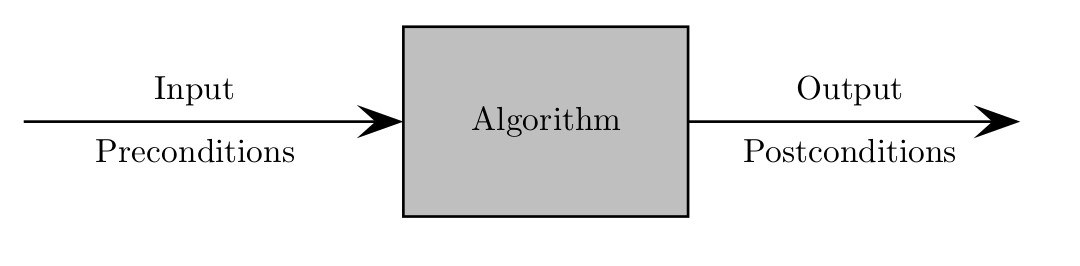
\includegraphics[width=0.8\textwidth]{png/contract}
	\caption{算法设计的契约。}
	\label{fig:contract}
\end{figure}
有了契约的概念,在算法设计的时候,明确算法的契约是非常重要的一步。
大到整个程序的框架,小至每个小模块的设计。
合理的算法契约在算法设计的时候不仅可以节省时间,
还可以让用户更快的了解该算法。

图 \ref{fig:bisection} 是求解非线性方程 $f(x)=0$ 时常用的二分法的算法契约。
其核心是每次将解的求解区间减半,直到近似解满足一定的条件。
输入中,$[a,b]$ 为算法开始给定的解的求解区间,$M$ 为最大的迭代次数,
$\epsilon, \delta $ 是两种不同的解的精度范围;
输出中, $c$ 是二分法得到的近似解,$h$ 是解所在的区间范围,
$k$ 为找到近似解所需要的迭代次数。
这里将二分法的具体实现看做一个黑盒子,
将细节忽略的好处是我们可以先更加专心的进行算法设计。
\begin{figure}[htbp]
	\centering
	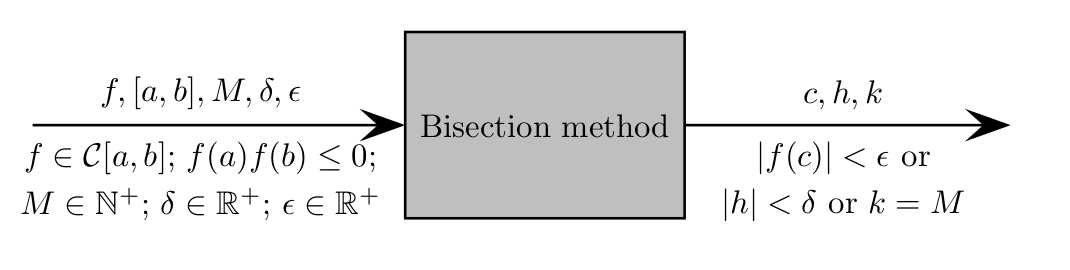
\includegraphics[width=0.8\textwidth]{png/bisectionMethod}
	\caption{求解非线性方程时常用的二分法的算法契约。}
	\label{fig:bisection}
\end{figure}
	
如果违反了先决条件,则该算法的行为或输出不确定。
为了确保先决条件,
我们要么在算法内部显式检查它们(关键字 \textbf{Check} 显示),
要么将此职责转移给用户(关键字 \textbf{Require} 显示)。 
在测试程序时,
实质上是在提供参数满足先决条件的测试用例后测试后置条件是否成立。


%%% Local Variables:
%%% mode: latex
%%% TeX-master: "../Guide"
%%% End:


\section{更好的算法设计}
\label{sec:designAlgo}

科学发展的最终目的是为了解决现实问题。
为了搞明白其中的物理规律,我们从中抽象出来一个数学模型。
对于这个数学模型,如果我们有一个解析解,并且这个解析解能够很好的反映这个物理现象,
我们可以很高兴的说我们已经“解决”了或者至少“部分解决”了这个问题。
但是随着科学的发展,我们关心的问题逐渐从简单到复杂,从单一问题到多问题耦合。
在这种情况下,我们不得不做一些计算,去”逼近”这个神秘的解。
随着计算机硬件的逐渐发展,
利用计算机这个有力的工具和数学结合去解决具有实际意义的物理问题越来越显现出强大的力量。
本小节主要介绍一下算法设计中的经验与理念。

\subsection{数学转化为算法}
\begin{itemize}
\item \textbf{数学到编程:无限到有限的转换。}数学和计算机结合的关键是,
  对于一个数学问题,我们需要有一个算法的近似。
  当我们讨论一个数学对象时,我们的表示方式可能是无限维的,无穷多的。
  例如当我们讨论一个单位圆时,它的自由度是无穷多的(从点集的角度出发,它由无穷多个点构成)。
  但计算机的资源是有限的,我们不能把圆上的每个点都表示出来。
  因此我们需要将一个具有无穷维度的数学问题转化为一个能够用有限的计算机资源表示的问题。
  对于一个单位圆,我们可以用它的内接多边形或者阶梯型线段去近似它(图 \ref{fig:circle}),
  不难发现,随着多边形边数的逐渐增大,其近似程度也越来越高。
  \begin{figure}[htbp]
    \centering
    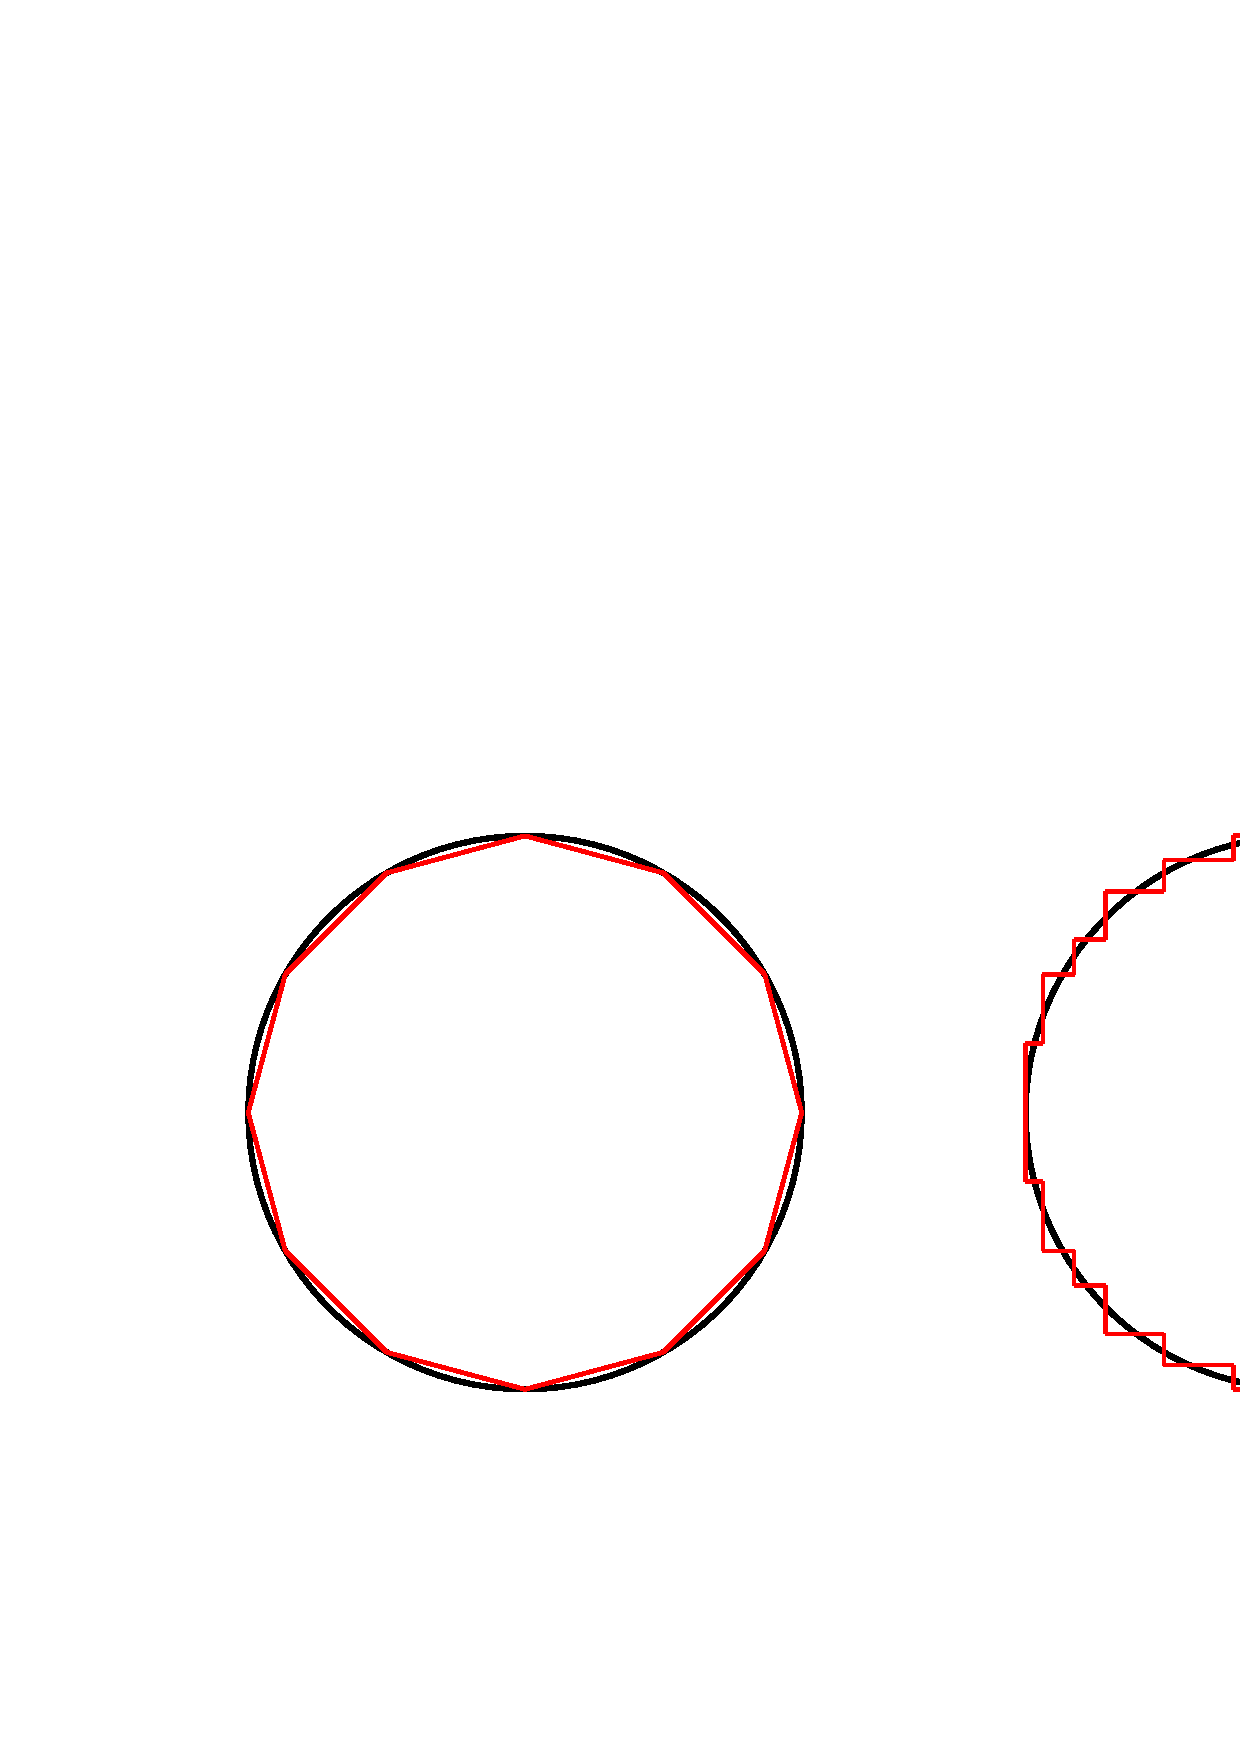
\includegraphics[width=0.40\textwidth]{eps/circle}
    \caption{ 不同图形拟合单位圆(左图为内接多边形,右图为阶梯型多边形)。\label{fig:circle}}
  \end{figure}		
\item \textbf{算法设计的原则:保证收敛,提高收敛率。}判断一个算法是否正确的原则是算法最终是否收敛。
  用$\epsilon-\delta$语言可以描述为:
  \begin{equation}
    \label{epsDel}
    \forall \epsilon >0, \;\; \exists \; N_0>0, \;\;\text{s.t.} \;\;
    \forall N > N_0, \;||E_N|| < \epsilon.
  \end{equation}
  这里,$\epsilon$ 表示想要控制的误差范围,
  $N_0$ 表示计算机资源(存储空间,运行时间等等),
  $E_N$ 表示近似模型与真实模型的误差。
  简单来说,收敛意味着想要多精确,就可以多精确,但是我们为之付出的代价可能会越来越大。
  当同一模型描述不同问题时,其收敛结果可能截然不同。
  假如我们仅仅想描述一个单位圆时,图 \ref{fig:circle} 的两种方式都可以达到目标;
  但当我们想利用近似的模型去逼近圆周长度时, 
  图 \ref{fig:circle} 右的近似方法显然是不收敛的。 
  这是因为不管用多么精细的阶梯型线段去拟合圆,其周长$l$始终满足$l \ge 8 > 2\pi$。
  另一个值得关心的概念是算法的收敛率,即一个收敛序列向其极限逼近的速度。
  在这里,我们可以看作是在相同的误差 $\epsilon$ 条件下,
  其最少投入的计算机资源 $N_0$ 的大小。$N_0$ 越小,其收敛率越高。
  而如何寻求一个合适的 $N_0$,是基于多方面因素的平衡。
\end{itemize}

\subsection{大问题到小问题的转换}
事实上,你面对的绝大多数问题往往不是你一下子就可以解决的。
在这时,学会将一个大的复杂的问题分解成小的简单的问题是一种很重要的科研能力。
虽然问题``小"的度量因人而异,但至少对你而言解决起来是相对轻松的。 
总体来说,我们应该遵循以下几个原则:
\begin{itemize}
\item \textbf{数学概念与C++类之间的简单对应。}在设计程序之前,
  请确保你已经将与程序相关的整个数学模型的概念与理论理解清楚,
  否则你会在接下来的设计中晕头转向。永远不要低估数学理论在程序设计中的重要性!
  接下来将数学中的基本概念直接映为相应的 C++ 类是一个很好的习惯, 
  这是因为在设计类时我们应遵循单一职责原则,
  即一个C++类尽量只完成一个任务或一些具有类似功能的任务。
\item \textbf{复杂类与简单类之间的交互一般放在复杂类中。}
\item \textbf{同级别类之间的交互可考虑放在一个算子类中。}
\item \textbf{每个小问题相对独立。}对问题进行分解利于我们将细节\emph{封装}(\emph{encapsulation})起来,
  这样我们就实现了将一个整体复杂度为$O(N)$的大问题转化为了若干个局部复杂度为$O(1)$的子问题。 
\end{itemize}

\subsection{关注模块的层级}
我们最后的设计中模块之间的层级关系应该如图\ref{fig:hierarchy}所示:
\begin{figure}[ht]
  \centering
  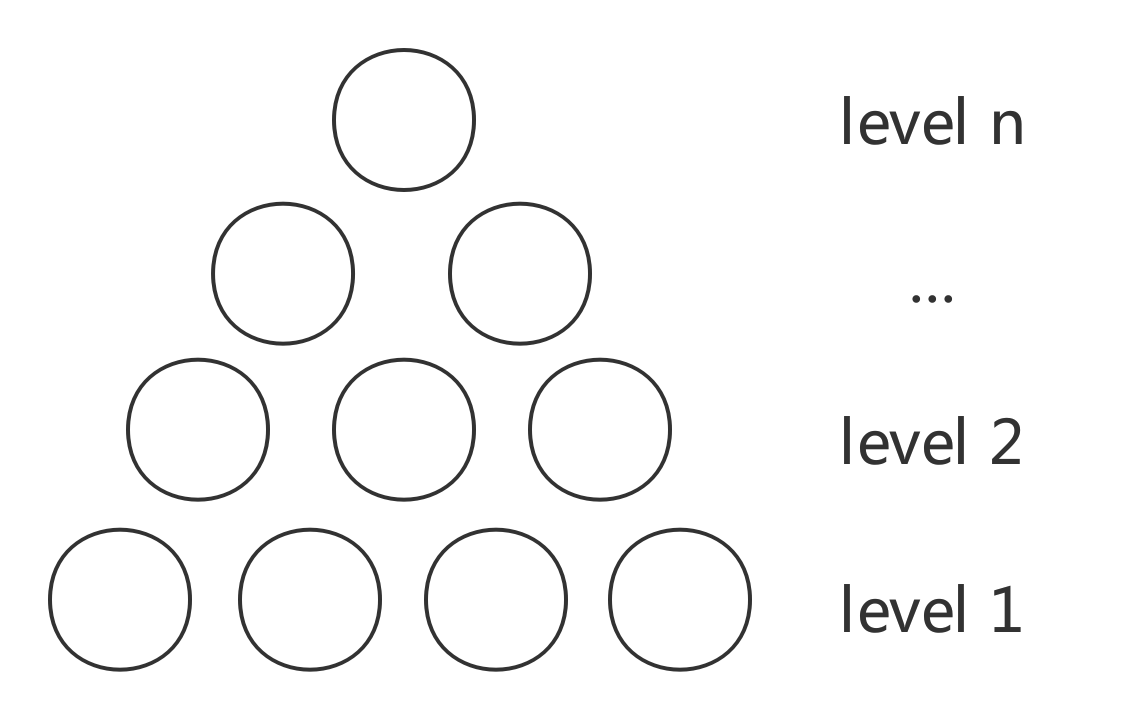
\includegraphics[width=0.30\textwidth]{png/hierarchy}
  \caption{模块间层级关系}
  \label{fig:hierarchy}
\end{figure}

其中最底层的模块主要负责将机器语言(例如某些数据结构,for循环等)
翻译成针对特定问题的语言(domain-specific language),
这里``domain" 对我们而言就是数学或者数学中一些最基本的概念。
底层的类实现机器语言和数学语言之间的转换,
使得我们的思考更集中于数学概念,而不用再考虑机器底层的细节。
在设计完成底层模块后,上层模块不宜再直接使用机器语言,
此时我们更应该从数学的角度思考问题。
正如Eckel所言:
\begin{quote}
  Create high-level abstractions to express what you're doing 
  and spend less time saying how you're doing it.
  The how has been solved once and for all and 
  is hidden in the algorithm's code, ready to be reused on demand.
\end{quote} 
在解决上层模块问题时,我们应该要牢记底层模块的契约而忘掉底层模块的具体实现细节。
底层模块与上层模块之间的关系正如学习英语时字母,单词,语句之间的关系。 
看书我们不能一个字母一个字母去看,而要一个单词一个单词去看,
学习一定时间后还需要一个句子一个句子去看。

\subsection{写好一个合格的设计文档}
整体设计完成后不要直接去写程序,先用\LaTeX{}写一个文档(\textbf{写下来!})。
其主要目的是为了确保算法设计的正确性。
在这个文档中,我们需要考虑:
\begin{itemize}
\item \textbf{整体设计的合理性。}比如:设计过程中层级是否明确?
  每个类中的成员变量是不是它的固有属性?
  算法的整体复杂度是否最小?
  重用是否发挥到最大化?
  未来需求有变化时,我们是否能够应对?等等。
\item \textbf{局部设计的规范性。}如果你已经对整体设计有一个宏观的把握, 
  已经将这个看似庞大的问题切割为一些等待解决的相互独立的小问题。
  面对这些小问题,你需要做的是:
  \begin{itemize}
  \item \emph{明确契约}
  \item \emph{设计算法}
  \item \emph{证明正确性}
  \item \emph{足够细化}
  \item \emph{写文档}
  \item \emph{程序实现}
  \item \emph{再测试}
  \end{itemize}
\end{itemize} 

\begin{remark}
在刚开始的学习阶段,我们应该严格按照上述形式进行训练。将自己的想法一步步严格写下来!
\end{remark}

\subsection{编程与调试}
编程与调试是算法设计的最后一步,而不是为了完成作业匆匆开始的第一步。
只有在熟悉整个程序设计过程,写出一份合格的设计文档后我们才开始进入编程与调试环节。
调试主要分为两种,
\begin{itemize}
\item \textbf{单一测试:}根据模块的层级,分别实现每个底层模块,
  测试这些模块,再写出这些底层模块耦合形成的模块并进行测试。 
\item \textbf{功能测试:}检查软件或者程序设计是否达到用户要求的功能。 
\end{itemize}
在有之前的准备后我们的目标应该如孙子兵法所言:不战而胜。 
好的设计,通常不需要太多时间调试!


%%% Local Variables:
%%% mode: latex
%%% TeX-master: "../Guide"
%%% End:


\section{C++ 中的代码重用---继承和组合}
\label{sec:reuse}

C++ 中最引人注目的功能之一是代码的重用,
当然这意味着不仅仅是对代码进行简单的复制和更改。
如何更好的实现代码的重用?
这与 C++ 中的大多数内容一样,解决方案围绕类(class)。 
我们可以通过创建新的类来重用代码,
但是可以使用其他人已经构建和调试的现有类,
而不是从头开始创建它们。
其优势在于我们可以不污染现有代码的前提下使用这些新的类。

实现代码重用的两个有效手段是
继承(inheritance)和组合(composition)。
组合是指新类中的成员是另一个或多个现有类的对象。
之所以称为组合,是因为新类是由现有类的对象组成。
更普遍的说,是 has-a 的关系,
例如汽车具有(has-a)引擎(见图 \ref{fig:has-a})。
\begin{figure}[htbp]
  \centering
  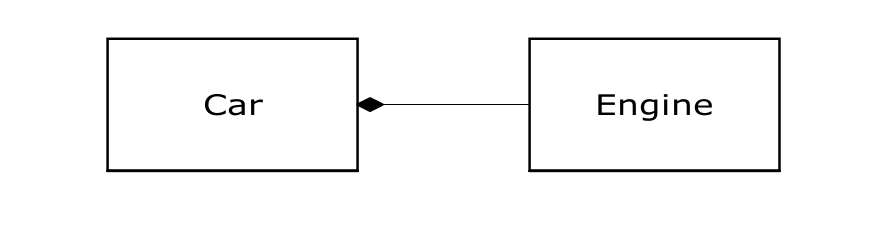
\includegraphics[width=0.5\textwidth]{png/has-a}
  \caption{C++ 中 has-a 的关系。}
  \label{fig:has-a}
\end{figure}
组合具有很大的灵活性。
因为新类的成员对象通常是私有的,
这使得使用该类的客户端程序员无法访问它们。
这方便让我们更改那些成员而不会打扰现有的客户端代码。
同时由于其简单,灵活,我们在程序设计中应该首先考虑。

继承是直接采用现有类的形式并向其中添加代码,而无需修改现有类。
如果更改了原始类(称为基类或者父类),
则继承后的类(称为派生类或者子类)也反映了这些变化。
这两种类型可以具有共同的特征和行为,
同时一种类型可能比另一种包含更多特征并且还可以处理更多消息。
我们也称之为 is-a 的关系。
图 \ref{fig:is-a} 是计算机辅助设计中经常遇见的形状案例。
基本类型是形状,每个形状都有大小,颜色,位置,
并且可以绘制,删除,移动,着色等,
从中派生特定类型的形状:圆形,正方形,三角形等,
每种形状可能具有其他特征和行为。 
例如,当你要计算形状的面积时,某些行为可能会有所不同。
\begin{figure}[htbp]
	\centering
	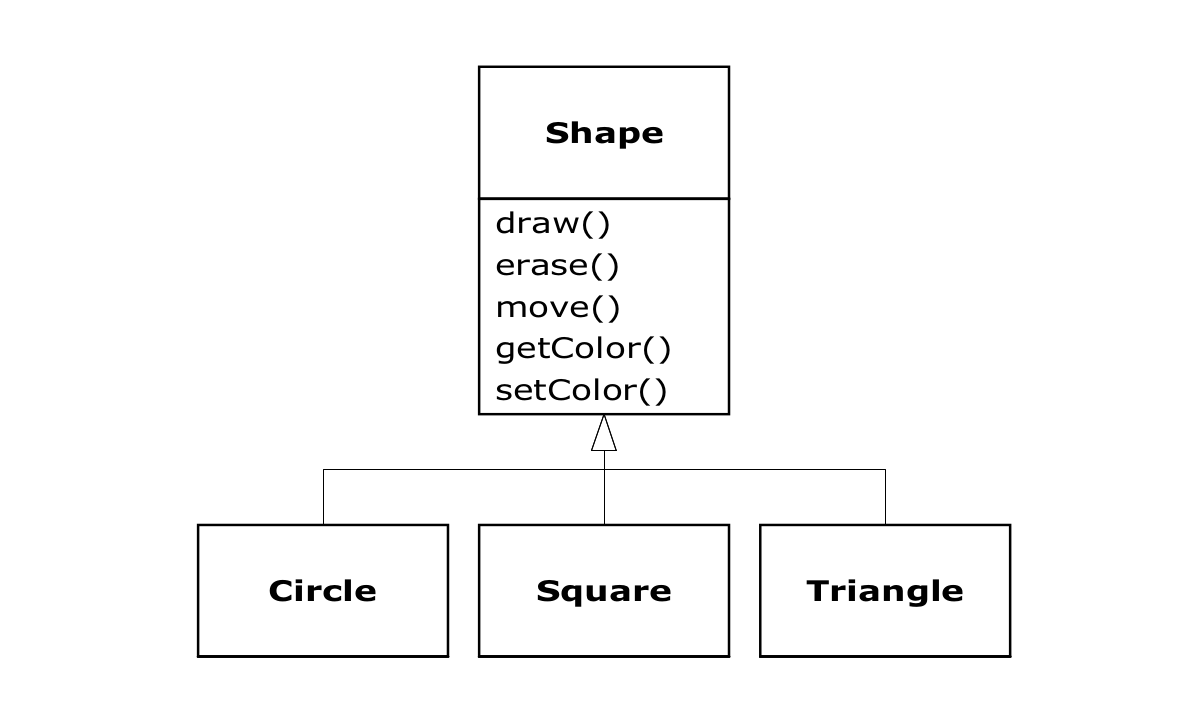
\includegraphics[width=0.5\textwidth]{png/is-a}
	\caption{C++ 中 is-a 的关系。}
	\label{fig:is-a}
\end{figure}

在这里我们只是强调一下这两个概念的重要性
而不去过多的解读它们。
如果你想系统的学习 C++,可以参考书籍
\begin{itemize}
	\item Thinking in C++, Volume 1: Introduction to Standard C++
		\cite{eckel2000thinking};
	\item Thinking in C++, Volume 2 : Practical Programming
		\cite{eckel2004thinking}。
\end{itemize}

\begin{remark}
	因为继承和组合在面向对象的编程中非常重要,
	我们这里不得不单独列一小结去高度强调它。
	在程序设计的时候应该首先考虑这两种关系,
	合理的运用,会使我们的设计更加简洁,灵活。
	但切记盲目使用,学会在实战中寻找经验!
\end{remark}






%%% Local Variables:
%%% mode: latex
%%% TeX-master: "../Guide"
%%% End:


 
{\footnotesize
\bibliographystyle{abbrv}
\bibliography{bib/Guide}
}



\end{CJK*}
\end{document}

%%% Local Variables:
%%% mode: latex
%%% TeX-master: t
%%% End:
